% Course project report (NeurIPS 2025 style, [final] option: names visible, no line numbers, no checklist).
% Build from this folder:  pdflatex main && bibtex main && pdflatex main && pdflatex main
% Numbers, macros, bibliography and figures are shared with ../paper (single source); nothing there is modified.
\documentclass{article}

\PassOptionsToPackage{numbers,sort&compress}{natbib}
\usepackage[final]{neurips_2025}

\usepackage[utf8]{inputenc}
\usepackage[T1]{fontenc}
\renewcommand{\ttdefault}{lmtt}
\usepackage{url}
\usepackage{booktabs}
\usepackage{amsmath}
\usepackage{amssymb}
\usepackage{amsfonts}
\usepackage{nicefrac}
\usepackage{microtype}
\usepackage{xcolor}
\usepackage{graphicx}
\usepackage{caption}
\usepackage{subcaption}

%% Minimal shims for ../paper/macros.tex, which assumes the packages and helpers that cvpr.sty provides.
\usepackage{xspace}
\usepackage[shortlabels,inline]{enumitem}
\makeatletter
\DeclareRobustCommand\onedot{\futurelet\@let@token\@onedot}
\def\@onedot{\ifx\@let@token.\else.\null\fi\xspace}
\providecommand{\eg}{\emph{e.g}\onedot}
\providecommand{\ie}{\emph{i.e}\onedot}
\providecommand{\etal}{\emph{et al}\onedot}
\makeatother

%% Packages and macros shared by main.tex and supplement.tex.
%% Load before hyperref (cvpr.sty already loads amsmath, amssymb, booktabs, graphicx, xcolor, natbib, caption, subcaption).

\usepackage{cuted}      % two-column teaser (official kit tweak)
\usepackage{currfile}   % \currfilebase for figure labels (official kit tweak)
\usepackage{amsthm}
\usepackage{multirow}
\usepackage{tikz}
\usetikzlibrary{arrows.meta,positioning,fit,calc,backgrounds}

%% ---------------------------------------------------------------------------
%% Draft annotations. ALL of these must be gone (or switched off) before submission.
%%   \verify{...}   unverified fact / citation detail          (red)
%%   \pending{...}  number or sentence waiting for an experiment (red, bold)
%%   \tbd           empty table cell waiting for final numbers  (red dash)
%%   \TODO{...}     writing to-do                                (red, bold)
%%   \prelim{...}   preliminary (descriptive) number; rendered orange while \ifshowprelim is true
%% ---------------------------------------------------------------------------
\newif\ifshowprelim
\showprelimtrue   % set to \showprelimfalse to render preliminary numbers in black
\newcommand{\verify}[1]{{\color{red}[VERIFY: #1]}}
\newcommand{\pending}[1]{{\color{red}\textbf{[#1]}}}
\newcommand{\tbd}{{\color{red}--}}
\newcommand{\TODO}[1]{{\color{red}\textbf{[TODO: #1]}}}
\newcommand{\prelim}[1]{\ifshowprelim{\color{orange}#1}\else#1\fi}
%   \placeholder{title}{text}  framed box for an experiment that is still running (red frame)
\newcommand{\placeholder}[2]{\par\smallskip\noindent\fcolorbox{red}{red!3}{\parbox{\dimexpr\linewidth-2\fboxsep-2\fboxrule\relax}{\footnotesize\color{red!55!black}\textbf{[PLACEHOLDER: #1]} #2}}\par\smallskip}

%% ---------------------------------------------------------------------------
%% Envelope placement: THE single switch. \envelopemaintrue keeps Sec. 4.6 (and Prop. 2) in the main paper;
%% \envelopemainfalse moves them to Supp. D and leaves a one-sentence pointer, a limitation sentence and no
%% A-dual+env row in the main paper. Recompile both main.tex and supplement.tex after changing it.
%% ---------------------------------------------------------------------------
\newif\ifenvelopemain
\envelopemaintrue
\newcommand{\envref}{\ifenvelopemain\cref{sec:env}\else Supp.~D\fi}

%% ---------------------------------------------------------------------------
%% Method names (rename here only).
%% ---------------------------------------------------------------------------
\newcommand{\mDual}{\textsf{A-dual}\xspace}
\newcommand{\mDualBoth}{\textsf{A-dual-both}\xspace}
\newcommand{\mDualEnv}{\textsf{A-dual+env}\xspace}
\newcommand{\mDistSplit}{\textsf{A-dist-split}\xspace}
\newcommand{\mDistBoth}{\textsf{A-dist-both}\xspace}
\newcommand{\mLocal}{\textsf{A-local}\xspace}
\newcommand{\mLocalSplit}{\textsf{A-local-split}\xspace}
\newcommand{\mSplitCP}{\textsf{split-CP}\xspace}
\newcommand{\omnidc}{OMNI-DC\xspace}

%% ---------------------------------------------------------------------------
%% Notation.
%% ---------------------------------------------------------------------------
\newcommand{\yhat}{\hat{y}}
\newcommand{\ytil}{\tilde{y}}
\newcommand{\dtil}{\tilde{d}}
\newcommand{\cA}{\mathcal{A}}
\newcommand{\cP}{\mathcal{P}}
\newcommand{\cS}{\mathcal{S}}
\newcommand{\cQ}{\mathcal{Q}}
\newcommand{\cU}{\mathcal{U}}
\newcommand{\cE}{\mathcal{E}}
\newcommand{\cB}{\mathcal{B}}
\newcommand{\qhat}{\hat{q}}
\newcommand{\sg}{s_{\gamma}}
\newcommand{\Cov}{\mathrm{Cov}}
\newcommand{\E}{\mathbb{E}}
\renewcommand{\P}{\mathbb{P}}
\newcommand{\1}{\mathbf{1}}
\newcommand{\med}{\operatorname{med}}
\newcommand{\BetaBin}{\operatorname{BetaBin}}
\newcommand{\BetaD}{\operatorname{Beta}}

%% Theorem environments (numbered within the paper; the supplement restates them with the same numbers).
\theoremstyle{plain}
\newtheorem{theorem}{Theorem}
\newtheorem{proposition}{Proposition}
\newtheorem{lemma}{Lemma}
\theoremstyle{remark}
\newtheorem{remark}{Remark}

%% =====================================================================================
%% numbers.tex -- every experimental number used in the text, as a macro.
%%
%% Status tags in the comments:
%%   [theory]   follows from the method's definition (exact or Monte Carlo of a known law); final.
%%   [data]     dataset statistic; final unless the preprocessing changes.
%%   [prelim]   descriptive number from the exploratory runs (3 splits x 2 draws, gamma chosen after a
%%              first NYU/KITTI run). Rendered via \prelim{} (orange while drafting). MUST be replaced by
%%              the confirmatory replication (20 scene/visit splits, paired bootstrap, >= 10 probe draws,
%%              gamma frozen) before any superiority claim is printed.
%%   [pending]  not yet available; renders as a red placeholder via \pending{}.
%%
%% Source keys: "UPD" = docs/REPORT_UPDATE_2026-11-02.md, "REP" = docs/PROJECT_REPORT.md.
%% Model set caveat for every E17 [prelim] number on NYU/KITTI and ARKitScenes: the "six pairs" are
%% {NYU, KITTI} x {DA-V2, UniDepthV2, Depth Pro} (scripts/run_new.sh, E17_PAIRS default). This IS the paper's main
%% model set on NYU/KITTI; Metric3D v2 is supplement-only. Depth Pro is excluded on ARKitScenes only (not reproduced).
%% =====================================================================================

%% ---------- Motivation: scale error and structured-anchor failure (E11, E13) ----------
% REP 9.10 Finding 1 (E11, 5 seeds x 6 draws, six NYU/KITTI pairs incl. Depth Pro). [prelim]
\newcommand{\NumScaleVarLo}{\prelim{65}}
\newcommand{\NumScaleVarHi}{\prelim{79}}
% REP 9.16 (E13, 5 seeds x 3 draws): A-local coverage under clustered anchors, k = 20 and 200, range over pairs. [prelim]
\newcommand{\NumLocalClusterCovLo}{\prelim{0.26}}
\newcommand{\NumLocalClusterCovHi}{\prelim{0.47}}
% REP 9.16: A-local median relative width, clustered vs uniform anchors, k = 20. [prelim]
\newcommand{\NumLocalClusterWidthLo}{\prelim{0.020}}
\newcommand{\NumLocalClusterWidthHi}{\prelim{0.046}}
\newcommand{\NumLocalUnifWidthLo}{\prelim{0.15}}
\newcommand{\NumLocalUnifWidthHi}{\prelim{0.45}}
% REP 9.16: A-local coverage, near-only and scan-line (rows) layouts, range over pairs and k. [prelim]
\newcommand{\NumLocalNearCovLo}{\prelim{0.71}}
\newcommand{\NumLocalNearCovHi}{\prelim{0.79}}
\newcommand{\NumLocalRowsCovLo}{\prelim{0.87}}
\newcommand{\NumLocalRowsCovHi}{\prelim{0.89}}
% REP 7.4 (T8): A-local theoretical coverage with 20 uniform anchors (10 calibrate): 10/11. [theory]
\newcommand{\NumLocalTheoryTwenty}{0.909}
% REP 9.16 Finding 3: A-local, uniform anchors, k = 20: coverage next to an anchor (< 0.02 diag) vs beyond 0.2 diag. [prelim]
\newcommand{\NumLocalNearBinCovLo}{\prelim{0.93}}
\newcommand{\NumLocalNearBinCovHi}{\prelim{0.94}}
\newcommand{\NumLocalFarBinCovLo}{\prelim{0.61}}
\newcommand{\NumLocalFarBinCovHi}{\prelim{0.84}}

%% ---------- Dual-role calibration on NYU/KITTI (E17, UPD 9.22, job 46165) ----------
% UPD 9.22 Finding 2: A-dual median relative width vs A-dist-both, median over the six pairs, range over the
% 10 layout x k cells. [prelim]
\newcommand{\NumDualWidthGainLo}{\prelim{16}}
\newcommand{\NumDualWidthGainHi}{\prelim{69}}
% UPD 9.22: A-dual is >= 10 % narrower than A-dist-both on 6/6 pairs in every one of the 10 cells
% (the pre-registered method gate; coverage at its theoretical value). [prelim]
\newcommand{\NumDualGatePairs}{\prelim{6}}
\newcommand{\NumPairs}{6}
\newcommand{\NumCells}{10}
% UPD 9.22: A-dual image-averaged coverage, range over all cells (theory 19/21 = 0.905). [prelim]
\newcommand{\NumDualCovLo}{\prelim{0.902}}
\newcommand{\NumDualCovHi}{\prelim{0.907}}
% [theory] r/(n+1) with n = 20, alpha = 0.1: 19/21.
\newcommand{\NumDualCovTheory}{0.905}
% UPD 9.22: A-dual-both width vs A-dist-both (median over pairs, range over cells), gate cells passed,
% and interval score range over pairs (every pair, every cell). [prelim]
\newcommand{\NumDualBothWidthGainLo}{\prelim{2}}
\newcommand{\NumDualBothWidthGainHi}{\prelim{60}}
\newcommand{\NumDualBothCellsPass}{\prelim{8}}
\newcommand{\NumDualBothISGainLo}{\prelim{1}}
\newcommand{\NumDualBothISGainHi}{\prelim{48}}
% UPD 9.22: mean median relative widths over pairs and layouts, k = 50 / 200. [prelim]
\newcommand{\NumWDistSplitFifty}{\prelim{0.154}}
\newcommand{\NumWDistSplitTwoHundred}{\prelim{0.133}}
\newcommand{\NumWDualFifty}{\prelim{0.187}}
\newcommand{\NumWDualTwoHundred}{\prelim{0.161}}
\newcommand{\NumWDualBothFifty}{\prelim{0.225}}
\newcommand{\NumWDualBothTwoHundred}{\prelim{0.195}}
\newcommand{\NumWDistBothFifty}{\prelim{0.280}}
\newcommand{\NumWDistBothTwoHundred}{\prelim{0.281}}
% UPD 9.22: coverage A-dual-both / A-dist-both (means, k = 50). [prelim]
\newcommand{\NumCovDualBoth}{\prelim{0.959}}
\newcommand{\NumCovDistBoth}{\prelim{0.970}}
% UPD 9.22 Finding 5: coverage spread across distance bins holding >= 1 % of pixels, points, median over pairs,
% range over layout x k. [prelim]
\newcommand{\NumSpreadDualLo}{\prelim{3.9}}
\newcommand{\NumSpreadDualHi}{\prelim{12.3}}
\newcommand{\NumSpreadDualBothLo}{\prelim{1.3}}
\newcommand{\NumSpreadDualBothHi}{\prelim{2.2}}
% UPD 9.22 Finding 5: A-dual coverage, near layout k = 50, at 0.1-0.2 of the diagonal. [prelim]
\newcommand{\NumDualFarCov}{\prelim{0.81}}

%% ---------- Probe budget (T13 corollary) ----------
% [theory] Beta(r, n+1-r) large-population approximation of the exact beta-binomial law;
% p10 of single-draw per-image coverage, n = 10 / 20 / 40 (UPD 7.6; rechecked with scipy: 0.794/0.819/0.841).
\newcommand{\NumBetaPTenTen}{0.795}
\newcommand{\NumBetaPTenTwenty}{0.819}
\newcommand{\NumBetaPTenForty}{0.841}
% [theory] share of images below 0.85 when coverage is averaged over two independent probe draws (Monte Carlo).
\newcommand{\NumBetaShortTwoTen}{15.3}
\newcommand{\NumBetaShortTwoTwenty}{11.5}
\newcommand{\NumBetaShortTwoForty}{6.6}
% [theory] share below 0.85 for ONE probe draw (Beta CDF at 0.85): n = 10 / 20 / 40.
\newcommand{\NumBetaShortOneTen}{19.7}
\newcommand{\NumBetaShortOneTwenty}{17.6}
\newcommand{\NumBetaShortOneForty}{13.0}
% UPD 9.22 Finding 3: measured on NYU/KITTI (mean over pairs and layouts, k = 50) -- implementation check only. [prelim]
\newcommand{\NumMeasPTenTwenty}{\prelim{0.820}}
\newcommand{\NumMeasShortTwoTwenty}{\prelim{11.4}}

%% ---------- ARKitScenes (UPD 5, 9.23) ----------
% [data] depth-upsampling validation split after dropping one video without confidence maps.
\newcommand{\NumArkFrames}{5{,}594}
\newcommand{\NumArkVisits}{107}
\newcommand{\NumArkPixelsM}{23.8}
% [data] iPad vs Faro laser at drawn anchors: mean signed log error -0.0155 (iPad reads nearer).
\newcommand{\NumArkIpadOffset}{1.6}
% [data] share of pixels with ARKit confidence 2.
\newcommand{\NumArkConfTwo}{94.6}
% UPD 9.23 E0 (all frames). [prelim; final unless preprocessing changes]. Depth Pro aggregates deliberately omitted.
\newcommand{\NumArkUniAbsRel}{\prelim{0.120}}
\newcommand{\NumArkUniDeltaOne}{\prelim{0.882}}
\newcommand{\NumArkDavAbsRel}{\prelim{0.466}}
\newcommand{\NumArkDavDeltaOne}{\prelim{0.325}}
% UPD 9.22 Finding 3 (ARKitScenes, laser-valued probes, n = 20): short share (avg. of 2 draws) and p10.
% Recomputed 2 Nov WITHOUT Depth Pro: {DA-V2 indoor, UniDepthV2} x 5 layouts x k in {50, 200} (results/e17_p20_g05). [prelim]
\newcommand{\NumArkShortLo}{\prelim{10.5}}
\newcommand{\NumArkShortHi}{\prelim{12.1}}
\newcommand{\NumArkPTenLo}{\prelim{0.817}}
\newcommand{\NumArkPTenHi}{\prelim{0.821}}
% UPD 9.23 E16 (iPad-valued anchors, uniform, k = 200), UniDepthV2: within-image methods certify the sensor reading. [prelim]
\newcommand{\NumArkLocalIpadCovUni}{\prelim{0.854}}
\newcommand{\NumArkLscpIpadCovUni}{\prelim{0.548}}

%% ---------- E18: value-source factorial on ARKitScenes, frozen models, 20 seeds (running) ----------
% Uniform layout finished on the cluster, not yet pulled; cluster layout at 3/20 seeds.
% Truth coverage of A-dual, (structured-anchor source / probe source), uniform layout. [pending]
% NOTE: a 400-image smoke test gave ~0.52 truth coverage with iPad-valued probes -- do NOT print; wait for E18.
\newcommand{\NumEEighteenCovLL}{\pending{E18 cov.\ laser/laser}}
\newcommand{\NumEEighteenCovIL}{\pending{E18 cov.\ iPad/laser}}
\newcommand{\NumEEighteenCovLI}{\pending{E18 cov.\ laser/iPad}}
\newcommand{\NumEEighteenCovII}{\pending{E18 cov.\ iPad/iPad}}
% Sensor-error envelope (to run, CPU only). [pending]
\newcommand{\NumEnvTruthCov}{\pending{envelope truth cov.}}
\newcommand{\NumEnvISGain}{\pending{envelope IS gain vs \mDistBoth}}
\newcommand{\NumEnvAlphaS}{\pending{$\alpha_s$}}
\newcommand{\NumEnvAlphaE}{\pending{$\alpha_e$}}

%% ---------- E19: OMNI-DC centre on ARKitScenes (DONE, 3 seeds; exploratory) ----------
% results_omnidc/e19_summary_3seeds.csv: seeds 0-2 (visit splits), probe draw 0, k = 200 (180 structured + 20
% probes), alpha = 0.1, gamma = 0.5, UniDepthV2-L frozen; OMNI-DC v1.1 fed RGB + the 180 structured anchors.
% Table cells: \ENineteen{...} in the generated block below; derived text numbers: \NumOmni*, \NumCluster*, ...
\newcommand{\NumOmniSeeds}{3}
\newcommand{\NumOmniTestLo}{1{,}909}
\newcommand{\NumOmniTestHi}{1{,}945}
% Smoke test (8 images, NOT for the paper): AbsRel on unseen pixels ~0.6 % (180 uniform laser anchors),
% ~2.0 % (iPad anchors), ~4.3 % (clustered anchors). Full-set accuracy not yet computed. [pending]
\newcommand{\NumOmniAbsRelUniform}{\pending{OMNI-DC AbsRel, uniform}}
\newcommand{\NumOmniAbsRelCluster}{\pending{OMNI-DC AbsRel, cluster}}

%% ---------- Probe ablation n in {10, 40} (UPD 9.22 Finding 4) ----------
% A-dual median relative width, k = 50 / 200 (mean over pairs and layouts). [prelim]
\newcommand{\NumWDualTenFifty}{\prelim{0.202}}
\newcommand{\NumWDualTenTwoHundred}{\prelim{0.178}}
\newcommand{\NumWDualFortyFifty}{\prelim{0.199}}
\newcommand{\NumWDualFortyTwoHundred}{\prelim{0.154}}
% A-dual short share with 40 probes (two-draw mean), range over k. [prelim]
\newcommand{\NumShortFortyLo}{\prelim{6.5}}
\newcommand{\NumShortFortyHi}{\prelim{6.8}}

%% ---------- Table lookups (values in the generated block) ----------
\newcommand{\ESeventeen}[3]{\ifcsname e17/#1/#2/#3\endcsname\prelim{\csname e17/#1/#2/#3\endcsname}\else\pending{?}\fi}
\newcommand{\ENineteen}[6]{\ifcsname e19/#1/#2/#3/#4/#5/#6\endcsname\prelim{\csname e19/#1/#2/#3/#4/#5/#6\endcsname}\else\pending{?}\fi}

%% ---------- Confirmatory protocol (design, final) ----------
\newcommand{\NumReplSplits}{20}
\newcommand{\NumProbeDraws}{10}

%% >>> GENERATED by tools/gen_numbers.py -- do not edit by hand
%% E17 (Tab. 2): \ESeventeen{layout}{k}{col}; col in local, dual, short, dW, bW, bIS.
%% local/dual = image-averaged coverage of A-local (all k structured anchors) / A-dual; short = % images
%% with single-draw coverage < 0.85, A-dual (pending until frac_img_short exists); dW/bW = % change in
%% median rel. width of A-dual / A-dual-both vs A-dist-both; bIS = % change in rel. interval score
%% (primary if available), A-dual-both vs A-dist-both. Median over the six pairs; lo / hi = min / max.
\expandafter\def\csname e17/uniform/50/local\endcsname{0.922}
\expandafter\def\csname e17/uniform/50/locallo\endcsname{0.922}
\expandafter\def\csname e17/uniform/50/localhi\endcsname{0.924}
\expandafter\def\csname e17/uniform/50/dual\endcsname{0.905}
\expandafter\def\csname e17/uniform/50/duallo\endcsname{0.904}
\expandafter\def\csname e17/uniform/50/dualhi\endcsname{0.907}
\expandafter\def\csname e17/uniform/50/short\endcsname{\pending{confirmatory}}
\expandafter\def\csname e17/uniform/50/shortlo\endcsname{\pending{confirmatory}}
\expandafter\def\csname e17/uniform/50/shorthi\endcsname{\pending{confirmatory}}
\expandafter\def\csname e17/uniform/50/dW\endcsname{$-$48}
\expandafter\def\csname e17/uniform/50/dWlo\endcsname{$-$52}
\expandafter\def\csname e17/uniform/50/dWhi\endcsname{$-$45}
\expandafter\def\csname e17/uniform/50/bW\endcsname{$-$37}
\expandafter\def\csname e17/uniform/50/bWlo\endcsname{$-$42}
\expandafter\def\csname e17/uniform/50/bWhi\endcsname{$-$24}
\expandafter\def\csname e17/uniform/50/bIS\endcsname{$-$28}
\expandafter\def\csname e17/uniform/50/bISlo\endcsname{$-$30}
\expandafter\def\csname e17/uniform/50/bIShi\endcsname{$-$20}
\expandafter\def\csname e17/uniform/200/local\endcsname{0.901}
\expandafter\def\csname e17/uniform/200/locallo\endcsname{0.901}
\expandafter\def\csname e17/uniform/200/localhi\endcsname{0.902}
\expandafter\def\csname e17/uniform/200/dual\endcsname{0.906}
\expandafter\def\csname e17/uniform/200/duallo\endcsname{0.904}
\expandafter\def\csname e17/uniform/200/dualhi\endcsname{0.907}
\expandafter\def\csname e17/uniform/200/short\endcsname{\pending{confirmatory}}
\expandafter\def\csname e17/uniform/200/shortlo\endcsname{\pending{confirmatory}}
\expandafter\def\csname e17/uniform/200/shorthi\endcsname{\pending{confirmatory}}
\expandafter\def\csname e17/uniform/200/dW\endcsname{$-$69}
\expandafter\def\csname e17/uniform/200/dWlo\endcsname{$-$71}
\expandafter\def\csname e17/uniform/200/dWhi\endcsname{$-$61}
\expandafter\def\csname e17/uniform/200/bW\endcsname{$-$60}
\expandafter\def\csname e17/uniform/200/bWlo\endcsname{$-$67}
\expandafter\def\csname e17/uniform/200/bWhi\endcsname{$-$46}
\expandafter\def\csname e17/uniform/200/bIS\endcsname{$-$46}
\expandafter\def\csname e17/uniform/200/bISlo\endcsname{$-$48}
\expandafter\def\csname e17/uniform/200/bIShi\endcsname{$-$36}
\expandafter\def\csname e17/rows/50/local\endcsname{0.899}
\expandafter\def\csname e17/rows/50/locallo\endcsname{0.895}
\expandafter\def\csname e17/rows/50/localhi\endcsname{0.901}
\expandafter\def\csname e17/rows/50/dual\endcsname{0.905}
\expandafter\def\csname e17/rows/50/duallo\endcsname{0.903}
\expandafter\def\csname e17/rows/50/dualhi\endcsname{0.905}
\expandafter\def\csname e17/rows/50/short\endcsname{\pending{confirmatory}}
\expandafter\def\csname e17/rows/50/shortlo\endcsname{\pending{confirmatory}}
\expandafter\def\csname e17/rows/50/shorthi\endcsname{\pending{confirmatory}}
\expandafter\def\csname e17/rows/50/dW\endcsname{$-$41}
\expandafter\def\csname e17/rows/50/dWlo\endcsname{$-$45}
\expandafter\def\csname e17/rows/50/dWhi\endcsname{$-$38}
\expandafter\def\csname e17/rows/50/bW\endcsname{$-$30}
\expandafter\def\csname e17/rows/50/bWlo\endcsname{$-$34}
\expandafter\def\csname e17/rows/50/bWhi\endcsname{$-$20}
\expandafter\def\csname e17/rows/50/bIS\endcsname{$-$24}
\expandafter\def\csname e17/rows/50/bISlo\endcsname{$-$26}
\expandafter\def\csname e17/rows/50/bIShi\endcsname{$-$18}
\expandafter\def\csname e17/rows/200/local\endcsname{0.873}
\expandafter\def\csname e17/rows/200/locallo\endcsname{0.870}
\expandafter\def\csname e17/rows/200/localhi\endcsname{0.876}
\expandafter\def\csname e17/rows/200/dual\endcsname{0.904}
\expandafter\def\csname e17/rows/200/duallo\endcsname{0.902}
\expandafter\def\csname e17/rows/200/dualhi\endcsname{0.905}
\expandafter\def\csname e17/rows/200/short\endcsname{\pending{confirmatory}}
\expandafter\def\csname e17/rows/200/shortlo\endcsname{\pending{confirmatory}}
\expandafter\def\csname e17/rows/200/shorthi\endcsname{\pending{confirmatory}}
\expandafter\def\csname e17/rows/200/dW\endcsname{$-$53}
\expandafter\def\csname e17/rows/200/dWlo\endcsname{$-$58}
\expandafter\def\csname e17/rows/200/dWhi\endcsname{$-$48}
\expandafter\def\csname e17/rows/200/bW\endcsname{$-$44}
\expandafter\def\csname e17/rows/200/bWlo\endcsname{$-$47}
\expandafter\def\csname e17/rows/200/bWhi\endcsname{$-$32}
\expandafter\def\csname e17/rows/200/bIS\endcsname{$-$32}
\expandafter\def\csname e17/rows/200/bISlo\endcsname{$-$35}
\expandafter\def\csname e17/rows/200/bIShi\endcsname{$-$24}
\expandafter\def\csname e17/cluster/50/local\endcsname{0.342}
\expandafter\def\csname e17/cluster/50/locallo\endcsname{0.312}
\expandafter\def\csname e17/cluster/50/localhi\endcsname{0.412}
\expandafter\def\csname e17/cluster/50/dual\endcsname{0.906}
\expandafter\def\csname e17/cluster/50/duallo\endcsname{0.905}
\expandafter\def\csname e17/cluster/50/dualhi\endcsname{0.907}
\expandafter\def\csname e17/cluster/50/short\endcsname{\pending{confirmatory}}
\expandafter\def\csname e17/cluster/50/shortlo\endcsname{\pending{confirmatory}}
\expandafter\def\csname e17/cluster/50/shorthi\endcsname{\pending{confirmatory}}
\expandafter\def\csname e17/cluster/50/dW\endcsname{$-$16}
\expandafter\def\csname e17/cluster/50/dWlo\endcsname{$-$23}
\expandafter\def\csname e17/cluster/50/dWhi\endcsname{$-$10}
\expandafter\def\csname e17/cluster/50/bW\endcsname{$-$2}
\expandafter\def\csname e17/cluster/50/bWlo\endcsname{$-$4}
\expandafter\def\csname e17/cluster/50/bWhi\endcsname{0}
\expandafter\def\csname e17/cluster/50/bIS\endcsname{$-$1}
\expandafter\def\csname e17/cluster/50/bISlo\endcsname{$-$10}
\expandafter\def\csname e17/cluster/50/bIShi\endcsname{$-$1}
\expandafter\def\csname e17/cluster/200/local\endcsname{0.397}
\expandafter\def\csname e17/cluster/200/locallo\endcsname{0.366}
\expandafter\def\csname e17/cluster/200/localhi\endcsname{0.463}
\expandafter\def\csname e17/cluster/200/dual\endcsname{0.905}
\expandafter\def\csname e17/cluster/200/duallo\endcsname{0.903}
\expandafter\def\csname e17/cluster/200/dualhi\endcsname{0.905}
\expandafter\def\csname e17/cluster/200/short\endcsname{\pending{confirmatory}}
\expandafter\def\csname e17/cluster/200/shortlo\endcsname{\pending{confirmatory}}
\expandafter\def\csname e17/cluster/200/shorthi\endcsname{\pending{confirmatory}}
\expandafter\def\csname e17/cluster/200/dW\endcsname{$-$17}
\expandafter\def\csname e17/cluster/200/dWlo\endcsname{$-$24}
\expandafter\def\csname e17/cluster/200/dWhi\endcsname{$-$11}
\expandafter\def\csname e17/cluster/200/bW\endcsname{$-$3}
\expandafter\def\csname e17/cluster/200/bWlo\endcsname{$-$6}
\expandafter\def\csname e17/cluster/200/bWhi\endcsname{$-$0}
\expandafter\def\csname e17/cluster/200/bIS\endcsname{$-$4}
\expandafter\def\csname e17/cluster/200/bISlo\endcsname{$-$11}
\expandafter\def\csname e17/cluster/200/bIShi\endcsname{$-$1}
\expandafter\def\csname e17/edges/50/local\endcsname{0.960}
\expandafter\def\csname e17/edges/50/locallo\endcsname{0.939}
\expandafter\def\csname e17/edges/50/localhi\endcsname{0.967}
\expandafter\def\csname e17/edges/50/dual\endcsname{0.905}
\expandafter\def\csname e17/edges/50/duallo\endcsname{0.904}
\expandafter\def\csname e17/edges/50/dualhi\endcsname{0.906}
\expandafter\def\csname e17/edges/50/short\endcsname{\pending{confirmatory}}
\expandafter\def\csname e17/edges/50/shortlo\endcsname{\pending{confirmatory}}
\expandafter\def\csname e17/edges/50/shorthi\endcsname{\pending{confirmatory}}
\expandafter\def\csname e17/edges/50/dW\endcsname{$-$24}
\expandafter\def\csname e17/edges/50/dWlo\endcsname{$-$27}
\expandafter\def\csname e17/edges/50/dWhi\endcsname{$-$13}
\expandafter\def\csname e17/edges/50/bW\endcsname{$-$12}
\expandafter\def\csname e17/edges/50/bWlo\endcsname{$-$16}
\expandafter\def\csname e17/edges/50/bWhi\endcsname{$-$3}
\expandafter\def\csname e17/edges/50/bIS\endcsname{$-$15}
\expandafter\def\csname e17/edges/50/bISlo\endcsname{$-$16}
\expandafter\def\csname e17/edges/50/bIShi\endcsname{$-$6}
\expandafter\def\csname e17/edges/200/local\endcsname{0.948}
\expandafter\def\csname e17/edges/200/locallo\endcsname{0.922}
\expandafter\def\csname e17/edges/200/localhi\endcsname{0.960}
\expandafter\def\csname e17/edges/200/dual\endcsname{0.905}
\expandafter\def\csname e17/edges/200/duallo\endcsname{0.903}
\expandafter\def\csname e17/edges/200/dualhi\endcsname{0.905}
\expandafter\def\csname e17/edges/200/short\endcsname{\pending{confirmatory}}
\expandafter\def\csname e17/edges/200/shortlo\endcsname{\pending{confirmatory}}
\expandafter\def\csname e17/edges/200/shorthi\endcsname{\pending{confirmatory}}
\expandafter\def\csname e17/edges/200/dW\endcsname{$-$34}
\expandafter\def\csname e17/edges/200/dWlo\endcsname{$-$36}
\expandafter\def\csname e17/edges/200/dWhi\endcsname{$-$31}
\expandafter\def\csname e17/edges/200/bW\endcsname{$-$23}
\expandafter\def\csname e17/edges/200/bWlo\endcsname{$-$28}
\expandafter\def\csname e17/edges/200/bWhi\endcsname{$-$14}
\expandafter\def\csname e17/edges/200/bIS\endcsname{$-$18}
\expandafter\def\csname e17/edges/200/bISlo\endcsname{$-$25}
\expandafter\def\csname e17/edges/200/bIShi\endcsname{$-$17}
\expandafter\def\csname e17/near/50/local\endcsname{0.769}
\expandafter\def\csname e17/near/50/locallo\endcsname{0.754}
\expandafter\def\csname e17/near/50/localhi\endcsname{0.799}
\expandafter\def\csname e17/near/50/dual\endcsname{0.905}
\expandafter\def\csname e17/near/50/duallo\endcsname{0.904}
\expandafter\def\csname e17/near/50/dualhi\endcsname{0.906}
\expandafter\def\csname e17/near/50/short\endcsname{\pending{confirmatory}}
\expandafter\def\csname e17/near/50/shortlo\endcsname{\pending{confirmatory}}
\expandafter\def\csname e17/near/50/shorthi\endcsname{\pending{confirmatory}}
\expandafter\def\csname e17/near/50/dW\endcsname{$-$33}
\expandafter\def\csname e17/near/50/dWlo\endcsname{$-$46}
\expandafter\def\csname e17/near/50/dWhi\endcsname{$-$19}
\expandafter\def\csname e17/near/50/bW\endcsname{$-$18}
\expandafter\def\csname e17/near/50/bWlo\endcsname{$-$30}
\expandafter\def\csname e17/near/50/bWhi\endcsname{$-$11}
\expandafter\def\csname e17/near/50/bIS\endcsname{$-$18}
\expandafter\def\csname e17/near/50/bISlo\endcsname{$-$23}
\expandafter\def\csname e17/near/50/bIShi\endcsname{$-$14}
\expandafter\def\csname e17/near/200/local\endcsname{0.728}
\expandafter\def\csname e17/near/200/locallo\endcsname{0.712}
\expandafter\def\csname e17/near/200/localhi\endcsname{0.759}
\expandafter\def\csname e17/near/200/dual\endcsname{0.905}
\expandafter\def\csname e17/near/200/duallo\endcsname{0.903}
\expandafter\def\csname e17/near/200/dualhi\endcsname{0.906}
\expandafter\def\csname e17/near/200/short\endcsname{\pending{confirmatory}}
\expandafter\def\csname e17/near/200/shortlo\endcsname{\pending{confirmatory}}
\expandafter\def\csname e17/near/200/shorthi\endcsname{\pending{confirmatory}}
\expandafter\def\csname e17/near/200/dW\endcsname{$-$37}
\expandafter\def\csname e17/near/200/dWlo\endcsname{$-$52}
\expandafter\def\csname e17/near/200/dWhi\endcsname{$-$20}
\expandafter\def\csname e17/near/200/bW\endcsname{$-$22}
\expandafter\def\csname e17/near/200/bWlo\endcsname{$-$38}
\expandafter\def\csname e17/near/200/bWhi\endcsname{$-$12}
\expandafter\def\csname e17/near/200/bIS\endcsname{$-$20}
\expandafter\def\csname e17/near/200/bISlo\endcsname{$-$27}
\expandafter\def\csname e17/near/200/bIShi\endcsname{$-$13}
%% true while any E17 short cell is pending (Supp. ranges table then prints one marker, not [lo, hi])
\newif\ifESeventeenShortPending
\ESeventeenShortPendingtrue

%% E17 single-draw short share of A-dual (% images < 0.85, macro includes \%), range over pairs, layouts and k;
%% \pending{confirmatory} until the summaries carry frac_img_short (theory: 17.6 % at n = 20, 13.0 % at n = 40).
\newcommand{\NumESeventeenShort}{\pending{confirmatory}}
\newcommand{\NumESeventeenShortForty}{\pending{confirmatory}}
\newcommand{\NumArkShortOne}{\pending{confirmatory}}

%% E19 (Tab. 3, Supp.): \ENineteen{pattern}{centre}{anchor src}{probe src}{method}{col};
%% col in cov (truth coverage, image mean), ptten (p10 of per-image coverage, one draw), short (% images
%% < 0.85, one draw), wgt (median width / laser depth), is (rel. interval score: primary if the column
%% exists, else exploratory; then > 5.0 is a blow-up from a few pixels -> \pending),
%% uninf (% pixels with width > 10 y, only if frac_uninformative exists).
%% exploratory (seeds 0-2; not in the confirmatory E19c): cluster/omnidc/lidar/clean/A-dist-split, cluster/omnidc/lidar/clean/A-dual, cluster/omnidc/lidar/clean/A-dual-both, cluster/omnidc/lidar/clean/split-CP, cluster/omnidc/lidar/lidar/A-dist-split, cluster/omnidc/lidar/lidar/A-dual, cluster/omnidc/lidar/lidar/A-dual-both, cluster/omnidc/lidar/lidar/split-CP, uniform/omnidc/lidar/clean/A-dist-split, uniform/omnidc/lidar/clean/A-dual, uniform/omnidc/lidar/clean/A-dual-both, uniform/omnidc/lidar/clean/split-CP, uniform/omnidc/lidar/lidar/A-dist-split, uniform/omnidc/lidar/lidar/A-dual, uniform/omnidc/lidar/lidar/A-dual-both, uniform/omnidc/lidar/lidar/split-CP
\expandafter\def\csname e19/cluster/omnidc/clean/clean/A-dist-split/cov\endcsname{0.924}
\expandafter\def\csname e19/cluster/omnidc/clean/clean/A-dist-split/ptten\endcsname{0.757}
\expandafter\def\csname e19/cluster/omnidc/clean/clean/A-dist-split/short\endcsname{16.7}
\expandafter\def\csname e19/cluster/omnidc/clean/clean/A-dist-split/wgt\endcsname{0.391}
\expandafter\def\csname e19/cluster/omnidc/clean/clean/A-dist-split/is\endcsname{0.422}
\expandafter\def\csname e19/cluster/omnidc/clean/clean/A-dist-split/uninf\endcsname{0.2}
\expandafter\def\csname e19/cluster/omnidc/clean/clean/A-dual/cov\endcsname{0.905}
\expandafter\def\csname e19/cluster/omnidc/clean/clean/A-dual/ptten\endcsname{0.820}
\expandafter\def\csname e19/cluster/omnidc/clean/clean/A-dual/short\endcsname{17.4}
\expandafter\def\csname e19/cluster/omnidc/clean/clean/A-dual/wgt\endcsname{0.226}
\expandafter\def\csname e19/cluster/omnidc/clean/clean/A-dual/is\endcsname{0.311}
\expandafter\def\csname e19/cluster/omnidc/clean/clean/A-dual/uninf\endcsname{0.0}
\expandafter\def\csname e19/cluster/omnidc/clean/clean/A-dual-both/cov\endcsname{0.971}
\expandafter\def\csname e19/cluster/omnidc/clean/clean/A-dual-both/ptten\endcsname{0.917}
\expandafter\def\csname e19/cluster/omnidc/clean/clean/A-dual-both/short\endcsname{2.2}
\expandafter\def\csname e19/cluster/omnidc/clean/clean/A-dual-both/wgt\endcsname{0.403}
\expandafter\def\csname e19/cluster/omnidc/clean/clean/A-dual-both/is\endcsname{0.421}
\expandafter\def\csname e19/cluster/omnidc/clean/clean/A-dual-both/uninf\endcsname{0.2}
\expandafter\def\csname e19/cluster/omnidc/clean/clean/split-CP/cov\endcsname{0.895}
\expandafter\def\csname e19/cluster/omnidc/clean/clean/split-CP/ptten\endcsname{0.676}
\expandafter\def\csname e19/cluster/omnidc/clean/clean/split-CP/short\endcsname{23.7}
\expandafter\def\csname e19/cluster/omnidc/clean/clean/split-CP/wgt\endcsname{0.336}
\expandafter\def\csname e19/cluster/omnidc/clean/clean/split-CP/is\endcsname{0.374}
\expandafter\def\csname e19/cluster/omnidc/clean/clean/split-CP/uninf\endcsname{0.0}
\expandafter\def\csname e19/cluster/omnidc/clean/lidar/A-dist-split/cov\endcsname{0.924}
\expandafter\def\csname e19/cluster/omnidc/clean/lidar/A-dist-split/ptten\endcsname{0.757}
\expandafter\def\csname e19/cluster/omnidc/clean/lidar/A-dist-split/short\endcsname{16.7}
\expandafter\def\csname e19/cluster/omnidc/clean/lidar/A-dist-split/wgt\endcsname{0.391}
\expandafter\def\csname e19/cluster/omnidc/clean/lidar/A-dist-split/is\endcsname{0.422}
\expandafter\def\csname e19/cluster/omnidc/clean/lidar/A-dist-split/uninf\endcsname{0.2}
\expandafter\def\csname e19/cluster/omnidc/clean/lidar/A-dual/cov\endcsname{0.915}
\expandafter\def\csname e19/cluster/omnidc/clean/lidar/A-dual/ptten\endcsname{0.807}
\expandafter\def\csname e19/cluster/omnidc/clean/lidar/A-dual/short\endcsname{17.4}
\expandafter\def\csname e19/cluster/omnidc/clean/lidar/A-dual/wgt\endcsname{0.241}
\expandafter\def\csname e19/cluster/omnidc/clean/lidar/A-dual/is\endcsname{0.322}
\expandafter\def\csname e19/cluster/omnidc/clean/lidar/A-dual/uninf\endcsname{0.0}
\expandafter\def\csname e19/cluster/omnidc/clean/lidar/A-dual-both/cov\endcsname{0.971}
\expandafter\def\csname e19/cluster/omnidc/clean/lidar/A-dual-both/ptten\endcsname{0.912}
\expandafter\def\csname e19/cluster/omnidc/clean/lidar/A-dual-both/short\endcsname{3.1}
\expandafter\def\csname e19/cluster/omnidc/clean/lidar/A-dual-both/wgt\endcsname{0.403}
\expandafter\def\csname e19/cluster/omnidc/clean/lidar/A-dual-both/is\endcsname{0.423}
\expandafter\def\csname e19/cluster/omnidc/clean/lidar/A-dual-both/uninf\endcsname{0.2}
\expandafter\def\csname e19/cluster/omnidc/clean/lidar/split-CP/cov\endcsname{0.895}
\expandafter\def\csname e19/cluster/omnidc/clean/lidar/split-CP/ptten\endcsname{0.676}
\expandafter\def\csname e19/cluster/omnidc/clean/lidar/split-CP/short\endcsname{23.7}
\expandafter\def\csname e19/cluster/omnidc/clean/lidar/split-CP/wgt\endcsname{0.336}
\expandafter\def\csname e19/cluster/omnidc/clean/lidar/split-CP/is\endcsname{0.374}
\expandafter\def\csname e19/cluster/omnidc/clean/lidar/split-CP/uninf\endcsname{0.0}
\expandafter\def\csname e19/cluster/omnidc/lidar/clean/A-dist-split/cov\endcsname{0.922}
\expandafter\def\csname e19/cluster/omnidc/lidar/clean/A-dist-split/ptten\endcsname{0.747}
\expandafter\def\csname e19/cluster/omnidc/lidar/clean/A-dist-split/short\endcsname{17.2}
\expandafter\def\csname e19/cluster/omnidc/lidar/clean/A-dist-split/wgt\endcsname{0.391}
\expandafter\def\csname e19/cluster/omnidc/lidar/clean/A-dist-split/is\endcsname{0.589}
\expandafter\def\csname e19/cluster/omnidc/lidar/clean/A-dist-split/uninf\endcsname{--}
\expandafter\def\csname e19/cluster/omnidc/lidar/clean/A-dual/cov\endcsname{0.905}
\expandafter\def\csname e19/cluster/omnidc/lidar/clean/A-dual/ptten\endcsname{0.820}
\expandafter\def\csname e19/cluster/omnidc/lidar/clean/A-dual/short\endcsname{17.2}
\expandafter\def\csname e19/cluster/omnidc/lidar/clean/A-dual/wgt\endcsname{0.233}
\expandafter\def\csname e19/cluster/omnidc/lidar/clean/A-dual/is\endcsname{\pending{primary IS}} % mean 8.75e+03: blow-up
\expandafter\def\csname e19/cluster/omnidc/lidar/clean/A-dual/uninf\endcsname{--}
\expandafter\def\csname e19/cluster/omnidc/lidar/clean/A-dual-both/cov\endcsname{0.971}
\expandafter\def\csname e19/cluster/omnidc/lidar/clean/A-dual-both/ptten\endcsname{0.918}
\expandafter\def\csname e19/cluster/omnidc/lidar/clean/A-dual-both/short\endcsname{2.2}
\expandafter\def\csname e19/cluster/omnidc/lidar/clean/A-dual-both/wgt\endcsname{0.404}
\expandafter\def\csname e19/cluster/omnidc/lidar/clean/A-dual-both/is\endcsname{\pending{primary IS}} % mean 8.75e+03: blow-up
\expandafter\def\csname e19/cluster/omnidc/lidar/clean/A-dual-both/uninf\endcsname{--}
\expandafter\def\csname e19/cluster/omnidc/lidar/clean/split-CP/cov\endcsname{0.894}
\expandafter\def\csname e19/cluster/omnidc/lidar/clean/split-CP/ptten\endcsname{0.665}
\expandafter\def\csname e19/cluster/omnidc/lidar/clean/split-CP/short\endcsname{24.3}
\expandafter\def\csname e19/cluster/omnidc/lidar/clean/split-CP/wgt\endcsname{0.336}
\expandafter\def\csname e19/cluster/omnidc/lidar/clean/split-CP/is\endcsname{0.581}
\expandafter\def\csname e19/cluster/omnidc/lidar/clean/split-CP/uninf\endcsname{--}
\expandafter\def\csname e19/cluster/omnidc/lidar/lidar/A-dist-split/cov\endcsname{0.922}
\expandafter\def\csname e19/cluster/omnidc/lidar/lidar/A-dist-split/ptten\endcsname{0.747}
\expandafter\def\csname e19/cluster/omnidc/lidar/lidar/A-dist-split/short\endcsname{17.2}
\expandafter\def\csname e19/cluster/omnidc/lidar/lidar/A-dist-split/wgt\endcsname{0.391}
\expandafter\def\csname e19/cluster/omnidc/lidar/lidar/A-dist-split/is\endcsname{0.589}
\expandafter\def\csname e19/cluster/omnidc/lidar/lidar/A-dist-split/uninf\endcsname{--}
\expandafter\def\csname e19/cluster/omnidc/lidar/lidar/A-dual/cov\endcsname{0.881}
\expandafter\def\csname e19/cluster/omnidc/lidar/lidar/A-dual/ptten\endcsname{0.737}
\expandafter\def\csname e19/cluster/omnidc/lidar/lidar/A-dual/short\endcsname{29.7}
\expandafter\def\csname e19/cluster/omnidc/lidar/lidar/A-dual/wgt\endcsname{0.227}
\expandafter\def\csname e19/cluster/omnidc/lidar/lidar/A-dual/is\endcsname{\pending{primary IS}} % mean 1e+04: blow-up
\expandafter\def\csname e19/cluster/omnidc/lidar/lidar/A-dual/uninf\endcsname{--}
\expandafter\def\csname e19/cluster/omnidc/lidar/lidar/A-dual-both/cov\endcsname{0.968}
\expandafter\def\csname e19/cluster/omnidc/lidar/lidar/A-dual-both/ptten\endcsname{0.904}
\expandafter\def\csname e19/cluster/omnidc/lidar/lidar/A-dual-both/short\endcsname{3.9}
\expandafter\def\csname e19/cluster/omnidc/lidar/lidar/A-dual-both/wgt\endcsname{0.403}
\expandafter\def\csname e19/cluster/omnidc/lidar/lidar/A-dual-both/is\endcsname{\pending{primary IS}} % mean 1e+04: blow-up
\expandafter\def\csname e19/cluster/omnidc/lidar/lidar/A-dual-both/uninf\endcsname{--}
\expandafter\def\csname e19/cluster/omnidc/lidar/lidar/split-CP/cov\endcsname{0.894}
\expandafter\def\csname e19/cluster/omnidc/lidar/lidar/split-CP/ptten\endcsname{0.665}
\expandafter\def\csname e19/cluster/omnidc/lidar/lidar/split-CP/short\endcsname{24.3}
\expandafter\def\csname e19/cluster/omnidc/lidar/lidar/split-CP/wgt\endcsname{0.336}
\expandafter\def\csname e19/cluster/omnidc/lidar/lidar/split-CP/is\endcsname{0.581}
\expandafter\def\csname e19/cluster/omnidc/lidar/lidar/split-CP/uninf\endcsname{--}
\expandafter\def\csname e19/cluster/unidepth/clean/clean/A-dist-split/cov\endcsname{0.924}
\expandafter\def\csname e19/cluster/unidepth/clean/clean/A-dist-split/ptten\endcsname{0.837}
\expandafter\def\csname e19/cluster/unidepth/clean/clean/A-dist-split/short\endcsname{12.5}
\expandafter\def\csname e19/cluster/unidepth/clean/clean/A-dist-split/wgt\endcsname{0.071}
\expandafter\def\csname e19/cluster/unidepth/clean/clean/A-dist-split/is\endcsname{0.135}
\expandafter\def\csname e19/cluster/unidepth/clean/clean/A-dist-split/uninf\endcsname{0.0}
\expandafter\def\csname e19/cluster/unidepth/clean/clean/A-dual/cov\endcsname{0.905}
\expandafter\def\csname e19/cluster/unidepth/clean/clean/A-dual/ptten\endcsname{0.819}
\expandafter\def\csname e19/cluster/unidepth/clean/clean/A-dual/short\endcsname{17.6}
\expandafter\def\csname e19/cluster/unidepth/clean/clean/A-dual/wgt\endcsname{0.109}
\expandafter\def\csname e19/cluster/unidepth/clean/clean/A-dual/is\endcsname{0.182}
\expandafter\def\csname e19/cluster/unidepth/clean/clean/A-dual/uninf\endcsname{0.0}
\expandafter\def\csname e19/cluster/unidepth/clean/clean/A-dual-both/cov\endcsname{0.967}
\expandafter\def\csname e19/cluster/unidepth/clean/clean/A-dual-both/ptten\endcsname{0.930}
\expandafter\def\csname e19/cluster/unidepth/clean/clean/A-dual-both/short\endcsname{0.5}
\expandafter\def\csname e19/cluster/unidepth/clean/clean/A-dual-both/wgt\endcsname{0.126}
\expandafter\def\csname e19/cluster/unidepth/clean/clean/A-dual-both/is\endcsname{0.174}
\expandafter\def\csname e19/cluster/unidepth/clean/clean/A-dual-both/uninf\endcsname{0.0}
\expandafter\def\csname e19/cluster/unidepth/clean/clean/split-CP/cov\endcsname{0.897}
\expandafter\def\csname e19/cluster/unidepth/clean/clean/split-CP/ptten\endcsname{0.595}
\expandafter\def\csname e19/cluster/unidepth/clean/clean/split-CP/short\endcsname{14.6}
\expandafter\def\csname e19/cluster/unidepth/clean/clean/split-CP/wgt\endcsname{0.513}
\expandafter\def\csname e19/cluster/unidepth/clean/clean/split-CP/is\endcsname{0.529}
\expandafter\def\csname e19/cluster/unidepth/clean/clean/split-CP/uninf\endcsname{0.0}
\expandafter\def\csname e19/cluster/unidepth/clean/lidar/A-dist-split/cov\endcsname{0.925}
\expandafter\def\csname e19/cluster/unidepth/clean/lidar/A-dist-split/ptten\endcsname{0.840}
\expandafter\def\csname e19/cluster/unidepth/clean/lidar/A-dist-split/short\endcsname{12.0}
\expandafter\def\csname e19/cluster/unidepth/clean/lidar/A-dist-split/wgt\endcsname{0.090}
\expandafter\def\csname e19/cluster/unidepth/clean/lidar/A-dist-split/is\endcsname{0.152}
\expandafter\def\csname e19/cluster/unidepth/clean/lidar/A-dist-split/uninf\endcsname{0.0}
\expandafter\def\csname e19/cluster/unidepth/clean/lidar/A-dual/cov\endcsname{0.927}
\expandafter\def\csname e19/cluster/unidepth/clean/lidar/A-dual/ptten\endcsname{0.823}
\expandafter\def\csname e19/cluster/unidepth/clean/lidar/A-dual/short\endcsname{13.3}
\expandafter\def\csname e19/cluster/unidepth/clean/lidar/A-dual/wgt\endcsname{0.131}
\expandafter\def\csname e19/cluster/unidepth/clean/lidar/A-dual/is\endcsname{0.197}
\expandafter\def\csname e19/cluster/unidepth/clean/lidar/A-dual/uninf\endcsname{0.0}
\expandafter\def\csname e19/cluster/unidepth/clean/lidar/A-dual-both/cov\endcsname{0.971}
\expandafter\def\csname e19/cluster/unidepth/clean/lidar/A-dual-both/ptten\endcsname{0.932}
\expandafter\def\csname e19/cluster/unidepth/clean/lidar/A-dual-both/short\endcsname{0.9}
\expandafter\def\csname e19/cluster/unidepth/clean/lidar/A-dual-both/wgt\endcsname{0.148}
\expandafter\def\csname e19/cluster/unidepth/clean/lidar/A-dual-both/is\endcsname{0.193}
\expandafter\def\csname e19/cluster/unidepth/clean/lidar/A-dual-both/uninf\endcsname{0.0}
\expandafter\def\csname e19/cluster/unidepth/clean/lidar/split-CP/cov\endcsname{0.897}
\expandafter\def\csname e19/cluster/unidepth/clean/lidar/split-CP/ptten\endcsname{0.595}
\expandafter\def\csname e19/cluster/unidepth/clean/lidar/split-CP/short\endcsname{14.6}
\expandafter\def\csname e19/cluster/unidepth/clean/lidar/split-CP/wgt\endcsname{0.513}
\expandafter\def\csname e19/cluster/unidepth/clean/lidar/split-CP/is\endcsname{0.529}
\expandafter\def\csname e19/cluster/unidepth/clean/lidar/split-CP/uninf\endcsname{0.0}
\expandafter\def\csname e19/cluster/unidepth/lidar/clean/A-dist-split/cov\endcsname{0.942}
\expandafter\def\csname e19/cluster/unidepth/lidar/clean/A-dist-split/ptten\endcsname{0.868}
\expandafter\def\csname e19/cluster/unidepth/lidar/clean/A-dist-split/short\endcsname{7.0}
\expandafter\def\csname e19/cluster/unidepth/lidar/clean/A-dist-split/wgt\endcsname{0.098}
\expandafter\def\csname e19/cluster/unidepth/lidar/clean/A-dist-split/is\endcsname{0.152}
\expandafter\def\csname e19/cluster/unidepth/lidar/clean/A-dist-split/uninf\endcsname{0.0}
\expandafter\def\csname e19/cluster/unidepth/lidar/clean/A-dual/cov\endcsname{0.906}
\expandafter\def\csname e19/cluster/unidepth/lidar/clean/A-dual/ptten\endcsname{0.820}
\expandafter\def\csname e19/cluster/unidepth/lidar/clean/A-dual/short\endcsname{17.5}
\expandafter\def\csname e19/cluster/unidepth/lidar/clean/A-dual/wgt\endcsname{0.123}
\expandafter\def\csname e19/cluster/unidepth/lidar/clean/A-dual/is\endcsname{0.191}
\expandafter\def\csname e19/cluster/unidepth/lidar/clean/A-dual/uninf\endcsname{0.0}
\expandafter\def\csname e19/cluster/unidepth/lidar/clean/A-dual-both/cov\endcsname{0.972}
\expandafter\def\csname e19/cluster/unidepth/lidar/clean/A-dual-both/ptten\endcsname{0.938}
\expandafter\def\csname e19/cluster/unidepth/lidar/clean/A-dual-both/short\endcsname{0.3}
\expandafter\def\csname e19/cluster/unidepth/lidar/clean/A-dual-both/wgt\endcsname{0.146}
\expandafter\def\csname e19/cluster/unidepth/lidar/clean/A-dual-both/is\endcsname{0.188}
\expandafter\def\csname e19/cluster/unidepth/lidar/clean/A-dual-both/uninf\endcsname{0.0}
\expandafter\def\csname e19/cluster/unidepth/lidar/clean/split-CP/cov\endcsname{0.897}
\expandafter\def\csname e19/cluster/unidepth/lidar/clean/split-CP/ptten\endcsname{0.595}
\expandafter\def\csname e19/cluster/unidepth/lidar/clean/split-CP/short\endcsname{14.6}
\expandafter\def\csname e19/cluster/unidepth/lidar/clean/split-CP/wgt\endcsname{0.513}
\expandafter\def\csname e19/cluster/unidepth/lidar/clean/split-CP/is\endcsname{0.529}
\expandafter\def\csname e19/cluster/unidepth/lidar/clean/split-CP/uninf\endcsname{0.0}
\expandafter\def\csname e19/cluster/unidepth/lidar/lidar/A-dist-split/cov\endcsname{0.866}
\expandafter\def\csname e19/cluster/unidepth/lidar/lidar/A-dist-split/ptten\endcsname{0.746}
\expandafter\def\csname e19/cluster/unidepth/lidar/lidar/A-dist-split/short\endcsname{33.0}
\expandafter\def\csname e19/cluster/unidepth/lidar/lidar/A-dist-split/wgt\endcsname{0.081}
\expandafter\def\csname e19/cluster/unidepth/lidar/lidar/A-dist-split/is\endcsname{0.157}
\expandafter\def\csname e19/cluster/unidepth/lidar/lidar/A-dist-split/uninf\endcsname{0.0}
\expandafter\def\csname e19/cluster/unidepth/lidar/lidar/A-dual/cov\endcsname{0.848}
\expandafter\def\csname e19/cluster/unidepth/lidar/lidar/A-dual/ptten\endcsname{0.623}
\expandafter\def\csname e19/cluster/unidepth/lidar/lidar/A-dual/short\endcsname{33.6}
\expandafter\def\csname e19/cluster/unidepth/lidar/lidar/A-dual/wgt\endcsname{0.119}
\expandafter\def\csname e19/cluster/unidepth/lidar/lidar/A-dual/is\endcsname{0.209}
\expandafter\def\csname e19/cluster/unidepth/lidar/lidar/A-dual/uninf\endcsname{0.0}
\expandafter\def\csname e19/cluster/unidepth/lidar/lidar/A-dual-both/cov\endcsname{0.946}
\expandafter\def\csname e19/cluster/unidepth/lidar/lidar/A-dual-both/ptten\endcsname{0.882}
\expandafter\def\csname e19/cluster/unidepth/lidar/lidar/A-dual-both/short\endcsname{6.0}
\expandafter\def\csname e19/cluster/unidepth/lidar/lidar/A-dual-both/wgt\endcsname{0.137}
\expandafter\def\csname e19/cluster/unidepth/lidar/lidar/A-dual-both/is\endcsname{0.189}
\expandafter\def\csname e19/cluster/unidepth/lidar/lidar/A-dual-both/uninf\endcsname{0.0}
\expandafter\def\csname e19/cluster/unidepth/lidar/lidar/split-CP/cov\endcsname{0.897}
\expandafter\def\csname e19/cluster/unidepth/lidar/lidar/split-CP/ptten\endcsname{0.595}
\expandafter\def\csname e19/cluster/unidepth/lidar/lidar/split-CP/short\endcsname{14.6}
\expandafter\def\csname e19/cluster/unidepth/lidar/lidar/split-CP/wgt\endcsname{0.513}
\expandafter\def\csname e19/cluster/unidepth/lidar/lidar/split-CP/is\endcsname{0.529}
\expandafter\def\csname e19/cluster/unidepth/lidar/lidar/split-CP/uninf\endcsname{0.0}
\expandafter\def\csname e19/uniform/omnidc/clean/clean/A-dist-split/cov\endcsname{0.923}
\expandafter\def\csname e19/uniform/omnidc/clean/clean/A-dist-split/ptten\endcsname{0.850}
\expandafter\def\csname e19/uniform/omnidc/clean/clean/A-dist-split/short\endcsname{9.9}
\expandafter\def\csname e19/uniform/omnidc/clean/clean/A-dist-split/wgt\endcsname{0.026}
\expandafter\def\csname e19/uniform/omnidc/clean/clean/A-dist-split/is\endcsname{0.071}
\expandafter\def\csname e19/uniform/omnidc/clean/clean/A-dist-split/uninf\endcsname{0.0}
\expandafter\def\csname e19/uniform/omnidc/clean/clean/A-dual/cov\endcsname{0.904}
\expandafter\def\csname e19/uniform/omnidc/clean/clean/A-dual/ptten\endcsname{0.819}
\expandafter\def\csname e19/uniform/omnidc/clean/clean/A-dual/short\endcsname{17.8}
\expandafter\def\csname e19/uniform/omnidc/clean/clean/A-dual/wgt\endcsname{0.023}
\expandafter\def\csname e19/uniform/omnidc/clean/clean/A-dual/is\endcsname{0.074}
\expandafter\def\csname e19/uniform/omnidc/clean/clean/A-dual/uninf\endcsname{0.0}
\expandafter\def\csname e19/uniform/omnidc/clean/clean/A-dual-both/cov\endcsname{0.948}
\expandafter\def\csname e19/uniform/omnidc/clean/clean/A-dual-both/ptten\endcsname{0.902}
\expandafter\def\csname e19/uniform/omnidc/clean/clean/A-dual-both/short\endcsname{1.3}
\expandafter\def\csname e19/uniform/omnidc/clean/clean/A-dual-both/wgt\endcsname{0.032}
\expandafter\def\csname e19/uniform/omnidc/clean/clean/A-dual-both/is\endcsname{0.074}
\expandafter\def\csname e19/uniform/omnidc/clean/clean/A-dual-both/uninf\endcsname{0.0}
\expandafter\def\csname e19/uniform/omnidc/clean/clean/split-CP/cov\endcsname{0.897}
\expandafter\def\csname e19/uniform/omnidc/clean/clean/split-CP/ptten\endcsname{0.813}
\expandafter\def\csname e19/uniform/omnidc/clean/clean/split-CP/short\endcsname{20.7}
\expandafter\def\csname e19/uniform/omnidc/clean/clean/split-CP/wgt\endcsname{0.024}
\expandafter\def\csname e19/uniform/omnidc/clean/clean/split-CP/is\endcsname{0.073}
\expandafter\def\csname e19/uniform/omnidc/clean/clean/split-CP/uninf\endcsname{0.0}
\expandafter\def\csname e19/uniform/omnidc/clean/lidar/A-dist-split/cov\endcsname{0.923}
\expandafter\def\csname e19/uniform/omnidc/clean/lidar/A-dist-split/ptten\endcsname{0.851}
\expandafter\def\csname e19/uniform/omnidc/clean/lidar/A-dist-split/short\endcsname{9.9}
\expandafter\def\csname e19/uniform/omnidc/clean/lidar/A-dist-split/wgt\endcsname{0.026}
\expandafter\def\csname e19/uniform/omnidc/clean/lidar/A-dist-split/is\endcsname{0.071}
\expandafter\def\csname e19/uniform/omnidc/clean/lidar/A-dist-split/uninf\endcsname{0.0}
\expandafter\def\csname e19/uniform/omnidc/clean/lidar/A-dual/cov\endcsname{0.980}
\expandafter\def\csname e19/uniform/omnidc/clean/lidar/A-dual/ptten\endcsname{0.956}
\expandafter\def\csname e19/uniform/omnidc/clean/lidar/A-dual/short\endcsname{0.0}
\expandafter\def\csname e19/uniform/omnidc/clean/lidar/A-dual/wgt\endcsname{0.075}
\expandafter\def\csname e19/uniform/omnidc/clean/lidar/A-dual/is\endcsname{0.108}
\expandafter\def\csname e19/uniform/omnidc/clean/lidar/A-dual/uninf\endcsname{0.0}
\expandafter\def\csname e19/uniform/omnidc/clean/lidar/A-dual-both/cov\endcsname{0.980}
\expandafter\def\csname e19/uniform/omnidc/clean/lidar/A-dual-both/ptten\endcsname{0.957}
\expandafter\def\csname e19/uniform/omnidc/clean/lidar/A-dual-both/short\endcsname{0.0}
\expandafter\def\csname e19/uniform/omnidc/clean/lidar/A-dual-both/wgt\endcsname{0.075}
\expandafter\def\csname e19/uniform/omnidc/clean/lidar/A-dual-both/is\endcsname{0.108}
\expandafter\def\csname e19/uniform/omnidc/clean/lidar/A-dual-both/uninf\endcsname{0.0}
\expandafter\def\csname e19/uniform/omnidc/clean/lidar/split-CP/cov\endcsname{0.897}
\expandafter\def\csname e19/uniform/omnidc/clean/lidar/split-CP/ptten\endcsname{0.813}
\expandafter\def\csname e19/uniform/omnidc/clean/lidar/split-CP/short\endcsname{20.7}
\expandafter\def\csname e19/uniform/omnidc/clean/lidar/split-CP/wgt\endcsname{0.024}
\expandafter\def\csname e19/uniform/omnidc/clean/lidar/split-CP/is\endcsname{0.073}
\expandafter\def\csname e19/uniform/omnidc/clean/lidar/split-CP/uninf\endcsname{0.0}
\expandafter\def\csname e19/uniform/omnidc/lidar/clean/A-dist-split/cov\endcsname{0.545}
\expandafter\def\csname e19/uniform/omnidc/lidar/clean/A-dist-split/ptten\endcsname{0.330}
\expandafter\def\csname e19/uniform/omnidc/lidar/clean/A-dist-split/short\endcsname{97.9}
\expandafter\def\csname e19/uniform/omnidc/lidar/clean/A-dist-split/wgt\endcsname{0.036}
\expandafter\def\csname e19/uniform/omnidc/lidar/clean/A-dist-split/is\endcsname{0.199}
\expandafter\def\csname e19/uniform/omnidc/lidar/clean/A-dist-split/uninf\endcsname{--}
\expandafter\def\csname e19/uniform/omnidc/lidar/clean/A-dual/cov\endcsname{0.905}
\expandafter\def\csname e19/uniform/omnidc/lidar/clean/A-dual/ptten\endcsname{0.817}
\expandafter\def\csname e19/uniform/omnidc/lidar/clean/A-dual/short\endcsname{18.4}
\expandafter\def\csname e19/uniform/omnidc/lidar/clean/A-dual/wgt\endcsname{0.071}
\expandafter\def\csname e19/uniform/omnidc/lidar/clean/A-dual/is\endcsname{0.150}
\expandafter\def\csname e19/uniform/omnidc/lidar/clean/A-dual/uninf\endcsname{--}
\expandafter\def\csname e19/uniform/omnidc/lidar/clean/A-dual-both/cov\endcsname{0.907}
\expandafter\def\csname e19/uniform/omnidc/lidar/clean/A-dual-both/ptten\endcsname{0.822}
\expandafter\def\csname e19/uniform/omnidc/lidar/clean/A-dual-both/short\endcsname{17.1}
\expandafter\def\csname e19/uniform/omnidc/lidar/clean/A-dual-both/wgt\endcsname{0.072}
\expandafter\def\csname e19/uniform/omnidc/lidar/clean/A-dual-both/is\endcsname{0.150}
\expandafter\def\csname e19/uniform/omnidc/lidar/clean/A-dual-both/uninf\endcsname{--}
\expandafter\def\csname e19/uniform/omnidc/lidar/clean/split-CP/cov\endcsname{0.897}
\expandafter\def\csname e19/uniform/omnidc/lidar/clean/split-CP/ptten\endcsname{0.793}
\expandafter\def\csname e19/uniform/omnidc/lidar/clean/split-CP/short\endcsname{18.0}
\expandafter\def\csname e19/uniform/omnidc/lidar/clean/split-CP/wgt\endcsname{0.070}
\expandafter\def\csname e19/uniform/omnidc/lidar/clean/split-CP/is\endcsname{0.147}
\expandafter\def\csname e19/uniform/omnidc/lidar/clean/split-CP/uninf\endcsname{--}
\expandafter\def\csname e19/uniform/omnidc/lidar/lidar/A-dist-split/cov\endcsname{0.539}
\expandafter\def\csname e19/uniform/omnidc/lidar/lidar/A-dist-split/ptten\endcsname{0.323}
\expandafter\def\csname e19/uniform/omnidc/lidar/lidar/A-dist-split/short\endcsname{98.0}
\expandafter\def\csname e19/uniform/omnidc/lidar/lidar/A-dist-split/wgt\endcsname{0.035}
\expandafter\def\csname e19/uniform/omnidc/lidar/lidar/A-dist-split/is\endcsname{0.200}
\expandafter\def\csname e19/uniform/omnidc/lidar/lidar/A-dist-split/uninf\endcsname{--}
\expandafter\def\csname e19/uniform/omnidc/lidar/lidar/A-dual/cov\endcsname{0.486}
\expandafter\def\csname e19/uniform/omnidc/lidar/lidar/A-dual/ptten\endcsname{0.054}
\expandafter\def\csname e19/uniform/omnidc/lidar/lidar/A-dual/short\endcsname{81.6}
\expandafter\def\csname e19/uniform/omnidc/lidar/lidar/A-dual/wgt\endcsname{0.029}
\expandafter\def\csname e19/uniform/omnidc/lidar/lidar/A-dual/is\endcsname{0.228}
\expandafter\def\csname e19/uniform/omnidc/lidar/lidar/A-dual/uninf\endcsname{--}
\expandafter\def\csname e19/uniform/omnidc/lidar/lidar/A-dual-both/cov\endcsname{0.649}
\expandafter\def\csname e19/uniform/omnidc/lidar/lidar/A-dual-both/ptten\endcsname{0.370}
\expandafter\def\csname e19/uniform/omnidc/lidar/lidar/A-dual-both/short\endcsname{79.7}
\expandafter\def\csname e19/uniform/omnidc/lidar/lidar/A-dual-both/wgt\endcsname{0.041}
\expandafter\def\csname e19/uniform/omnidc/lidar/lidar/A-dual-both/is\endcsname{0.184}
\expandafter\def\csname e19/uniform/omnidc/lidar/lidar/A-dual-both/uninf\endcsname{--}
\expandafter\def\csname e19/uniform/omnidc/lidar/lidar/split-CP/cov\endcsname{0.897}
\expandafter\def\csname e19/uniform/omnidc/lidar/lidar/split-CP/ptten\endcsname{0.793}
\expandafter\def\csname e19/uniform/omnidc/lidar/lidar/split-CP/short\endcsname{18.0}
\expandafter\def\csname e19/uniform/omnidc/lidar/lidar/split-CP/wgt\endcsname{0.070}
\expandafter\def\csname e19/uniform/omnidc/lidar/lidar/split-CP/is\endcsname{0.147}
\expandafter\def\csname e19/uniform/omnidc/lidar/lidar/split-CP/uninf\endcsname{--}
\expandafter\def\csname e19/uniform/unidepth/clean/clean/A-dist-split/cov\endcsname{0.923}
\expandafter\def\csname e19/uniform/unidepth/clean/clean/A-dist-split/ptten\endcsname{0.860}
\expandafter\def\csname e19/uniform/unidepth/clean/clean/A-dist-split/short\endcsname{7.6}
\expandafter\def\csname e19/uniform/unidepth/clean/clean/A-dist-split/wgt\endcsname{0.027}
\expandafter\def\csname e19/uniform/unidepth/clean/clean/A-dist-split/is\endcsname{0.082}
\expandafter\def\csname e19/uniform/unidepth/clean/clean/A-dist-split/uninf\endcsname{0.0}
\expandafter\def\csname e19/uniform/unidepth/clean/clean/A-dual/cov\endcsname{0.904}
\expandafter\def\csname e19/uniform/unidepth/clean/clean/A-dual/ptten\endcsname{0.818}
\expandafter\def\csname e19/uniform/unidepth/clean/clean/A-dual/short\endcsname{17.7}
\expandafter\def\csname e19/uniform/unidepth/clean/clean/A-dual/wgt\endcsname{0.030}
\expandafter\def\csname e19/uniform/unidepth/clean/clean/A-dual/is\endcsname{0.089}
\expandafter\def\csname e19/uniform/unidepth/clean/clean/A-dual/uninf\endcsname{0.0}
\expandafter\def\csname e19/uniform/unidepth/clean/clean/A-dual-both/cov\endcsname{0.949}
\expandafter\def\csname e19/uniform/unidepth/clean/clean/A-dual-both/ptten\endcsname{0.905}
\expandafter\def\csname e19/uniform/unidepth/clean/clean/A-dual-both/short\endcsname{0.8}
\expandafter\def\csname e19/uniform/unidepth/clean/clean/A-dual-both/wgt\endcsname{0.038}
\expandafter\def\csname e19/uniform/unidepth/clean/clean/A-dual-both/is\endcsname{0.087}
\expandafter\def\csname e19/uniform/unidepth/clean/clean/A-dual-both/uninf\endcsname{0.0}
\expandafter\def\csname e19/uniform/unidepth/clean/clean/split-CP/cov\endcsname{0.897}
\expandafter\def\csname e19/uniform/unidepth/clean/clean/split-CP/ptten\endcsname{0.594}
\expandafter\def\csname e19/uniform/unidepth/clean/clean/split-CP/short\endcsname{14.5}
\expandafter\def\csname e19/uniform/unidepth/clean/clean/split-CP/wgt\endcsname{0.513}
\expandafter\def\csname e19/uniform/unidepth/clean/clean/split-CP/is\endcsname{0.528}
\expandafter\def\csname e19/uniform/unidepth/clean/clean/split-CP/uninf\endcsname{0.0}
\expandafter\def\csname e19/uniform/unidepth/clean/lidar/A-dist-split/cov\endcsname{0.924}
\expandafter\def\csname e19/uniform/unidepth/clean/lidar/A-dist-split/ptten\endcsname{0.864}
\expandafter\def\csname e19/uniform/unidepth/clean/lidar/A-dist-split/short\endcsname{6.4}
\expandafter\def\csname e19/uniform/unidepth/clean/lidar/A-dist-split/wgt\endcsname{0.030}
\expandafter\def\csname e19/uniform/unidepth/clean/lidar/A-dist-split/is\endcsname{0.083}
\expandafter\def\csname e19/uniform/unidepth/clean/lidar/A-dist-split/uninf\endcsname{0.0}
\expandafter\def\csname e19/uniform/unidepth/clean/lidar/A-dual/cov\endcsname{0.973}
\expandafter\def\csname e19/uniform/unidepth/clean/lidar/A-dual/ptten\endcsname{0.942}
\expandafter\def\csname e19/uniform/unidepth/clean/lidar/A-dual/short\endcsname{0.1}
\expandafter\def\csname e19/uniform/unidepth/clean/lidar/A-dual/wgt\endcsname{0.074}
\expandafter\def\csname e19/uniform/unidepth/clean/lidar/A-dual/is\endcsname{0.112}
\expandafter\def\csname e19/uniform/unidepth/clean/lidar/A-dual/uninf\endcsname{0.0}
\expandafter\def\csname e19/uniform/unidepth/clean/lidar/A-dual-both/cov\endcsname{0.975}
\expandafter\def\csname e19/uniform/unidepth/clean/lidar/A-dual-both/ptten\endcsname{0.946}
\expandafter\def\csname e19/uniform/unidepth/clean/lidar/A-dual-both/short\endcsname{0.0}
\expandafter\def\csname e19/uniform/unidepth/clean/lidar/A-dual-both/wgt\endcsname{0.074}
\expandafter\def\csname e19/uniform/unidepth/clean/lidar/A-dual-both/is\endcsname{0.113}
\expandafter\def\csname e19/uniform/unidepth/clean/lidar/A-dual-both/uninf\endcsname{0.0}
\expandafter\def\csname e19/uniform/unidepth/clean/lidar/split-CP/cov\endcsname{0.897}
\expandafter\def\csname e19/uniform/unidepth/clean/lidar/split-CP/ptten\endcsname{0.594}
\expandafter\def\csname e19/uniform/unidepth/clean/lidar/split-CP/short\endcsname{14.5}
\expandafter\def\csname e19/uniform/unidepth/clean/lidar/split-CP/wgt\endcsname{0.513}
\expandafter\def\csname e19/uniform/unidepth/clean/lidar/split-CP/is\endcsname{0.528}
\expandafter\def\csname e19/uniform/unidepth/clean/lidar/split-CP/uninf\endcsname{0.0}
\expandafter\def\csname e19/uniform/unidepth/lidar/clean/A-dist-split/cov\endcsname{0.616}
\expandafter\def\csname e19/uniform/unidepth/lidar/clean/A-dist-split/ptten\endcsname{0.390}
\expandafter\def\csname e19/uniform/unidepth/lidar/clean/A-dist-split/short\endcsname{93.7}
\expandafter\def\csname e19/uniform/unidepth/lidar/clean/A-dist-split/wgt\endcsname{0.035}
\expandafter\def\csname e19/uniform/unidepth/lidar/clean/A-dist-split/is\endcsname{0.144}
\expandafter\def\csname e19/uniform/unidepth/lidar/clean/A-dist-split/uninf\endcsname{0.0}
\expandafter\def\csname e19/uniform/unidepth/lidar/clean/A-dual/cov\endcsname{0.904}
\expandafter\def\csname e19/uniform/unidepth/lidar/clean/A-dual/ptten\endcsname{0.818}
\expandafter\def\csname e19/uniform/unidepth/lidar/clean/A-dual/short\endcsname{17.9}
\expandafter\def\csname e19/uniform/unidepth/lidar/clean/A-dual/wgt\endcsname{0.066}
\expandafter\def\csname e19/uniform/unidepth/lidar/clean/A-dual/is\endcsname{0.121}
\expandafter\def\csname e19/uniform/unidepth/lidar/clean/A-dual/uninf\endcsname{0.0}
\expandafter\def\csname e19/uniform/unidepth/lidar/clean/A-dual-both/cov\endcsname{0.912}
\expandafter\def\csname e19/uniform/unidepth/lidar/clean/A-dual-both/ptten\endcsname{0.836}
\expandafter\def\csname e19/uniform/unidepth/lidar/clean/A-dual-both/short\endcsname{13.4}
\expandafter\def\csname e19/uniform/unidepth/lidar/clean/A-dual-both/wgt\endcsname{0.068}
\expandafter\def\csname e19/uniform/unidepth/lidar/clean/A-dual-both/is\endcsname{0.120}
\expandafter\def\csname e19/uniform/unidepth/lidar/clean/A-dual-both/uninf\endcsname{0.0}
\expandafter\def\csname e19/uniform/unidepth/lidar/clean/split-CP/cov\endcsname{0.897}
\expandafter\def\csname e19/uniform/unidepth/lidar/clean/split-CP/ptten\endcsname{0.594}
\expandafter\def\csname e19/uniform/unidepth/lidar/clean/split-CP/short\endcsname{14.5}
\expandafter\def\csname e19/uniform/unidepth/lidar/clean/split-CP/wgt\endcsname{0.513}
\expandafter\def\csname e19/uniform/unidepth/lidar/clean/split-CP/is\endcsname{0.528}
\expandafter\def\csname e19/uniform/unidepth/lidar/clean/split-CP/uninf\endcsname{0.0}
\expandafter\def\csname e19/uniform/unidepth/lidar/lidar/A-dist-split/cov\endcsname{0.527}
\expandafter\def\csname e19/uniform/unidepth/lidar/lidar/A-dist-split/ptten\endcsname{0.284}
\expandafter\def\csname e19/uniform/unidepth/lidar/lidar/A-dist-split/short\endcsname{97.0}
\expandafter\def\csname e19/uniform/unidepth/lidar/lidar/A-dist-split/wgt\endcsname{0.033}
\expandafter\def\csname e19/uniform/unidepth/lidar/lidar/A-dist-split/is\endcsname{0.168}
\expandafter\def\csname e19/uniform/unidepth/lidar/lidar/A-dist-split/uninf\endcsname{0.0}
\expandafter\def\csname e19/uniform/unidepth/lidar/lidar/A-dual/cov\endcsname{0.565}
\expandafter\def\csname e19/uniform/unidepth/lidar/lidar/A-dual/ptten\endcsname{0.108}
\expandafter\def\csname e19/uniform/unidepth/lidar/lidar/A-dual/short\endcsname{73.8}
\expandafter\def\csname e19/uniform/unidepth/lidar/lidar/A-dual/wgt\endcsname{0.036}
\expandafter\def\csname e19/uniform/unidepth/lidar/lidar/A-dual/is\endcsname{0.174}
\expandafter\def\csname e19/uniform/unidepth/lidar/lidar/A-dual/uninf\endcsname{0.0}
\expandafter\def\csname e19/uniform/unidepth/lidar/lidar/A-dual-both/cov\endcsname{0.666}
\expandafter\def\csname e19/uniform/unidepth/lidar/lidar/A-dual-both/ptten\endcsname{0.326}
\expandafter\def\csname e19/uniform/unidepth/lidar/lidar/A-dual-both/short\endcsname{70.2}
\expandafter\def\csname e19/uniform/unidepth/lidar/lidar/A-dual-both/wgt\endcsname{0.045}
\expandafter\def\csname e19/uniform/unidepth/lidar/lidar/A-dual-both/is\endcsname{0.150}
\expandafter\def\csname e19/uniform/unidepth/lidar/lidar/A-dual-both/uninf\endcsname{0.0}
\expandafter\def\csname e19/uniform/unidepth/lidar/lidar/split-CP/cov\endcsname{0.897}
\expandafter\def\csname e19/uniform/unidepth/lidar/lidar/split-CP/ptten\endcsname{0.594}
\expandafter\def\csname e19/uniform/unidepth/lidar/lidar/split-CP/short\endcsname{14.5}
\expandafter\def\csname e19/uniform/unidepth/lidar/lidar/split-CP/wgt\endcsname{0.513}
\expandafter\def\csname e19/uniform/unidepth/lidar/lidar/split-CP/is\endcsname{0.528}
\expandafter\def\csname e19/uniform/unidepth/lidar/lidar/split-CP/uninf\endcsname{0.0}
%% true when the E19 summary carries frac_uninformative (Supp. Tab. S2 then shows an Uninf. column)
\newif\ifENineteenUninf
\ENineteenUninftrue
%% Per-seed mean-over-images rel. IS of the blow-up cells -- NOT for the paper (primary IS is the image median):
%%   cluster/omnidc/clean/clean/A-dist-split: 0.591 / 0.56 / 2.98e+15 / 4.9e+21 / 5.76e+28 / 1.32e+12 / 0.584 / 5.57e+28 / 1.14e+11 / 2.98e+10
%%   cluster/omnidc/clean/clean/A-dual: 0.387 / 0.38 / 0.389 / 0.384 / 0.381 / 0.391 / 0.382 / 0.395 / 0.771 / 2.5e+21
%%   cluster/omnidc/clean/clean/A-dual-both: 0.505 / 0.502 / 2.98e+15 / 4.9e+21 / 5.76e+28 / 1.32e+12 / 0.506 / 5.57e+28 / 1.14e+11 / 2.5e+21
%%   cluster/omnidc/clean/lidar/A-dist-split: 0.591 / 0.56 / 8.97e+15 / 4.9e+21 / 2.01e+29 / 1.21e+12 / 0.584 / 9.25e+28 / 1.14e+11 / 2.91e+10
%%   cluster/omnidc/clean/lidar/A-dual: 0.4 / 0.393 / 0.402 / 0.396 / 0.393 / 0.403 / 0.393 / 0.408 / 0.643 / 5.62e+20
%%   cluster/omnidc/clean/lidar/A-dual-both: 0.511 / 0.507 / 8.97e+15 / 4.9e+21 / 2.01e+29 / 1.21e+12 / 0.509 / 9.25e+28 / 1.14e+11 / 5.62e+20

%% E19 derived numbers for the text (uniform/cluster, k = 200, laser anchors and probes unless stated).
% OMNI-DC centres (split-CP / A-dual / A-dist-split) vs UniDepthV2 A-dual, uniform: rel. IS lower by 18.1, 16.1, 20.2 %
\newcommand{\NumOmniGainLo}{16}
\newcommand{\NumOmniGainHi}{20}
% A-dual on OMNI-DC vs split-CP on OMNI-DC, uniform: rel. IS +2.5 %
\newcommand{\NumOmniDualCost}{2.5}
% cluster: UniDepthV2 A-dual vs OMNI-DC A-dual / split-CP: rel. IS lower by 41.4 / 51.4 %
\newcommand{\NumClusterGainDual}{41}
\newcommand{\NumClusterGainCP}{51}
% raw UniDepthV2 split-CP (no anchors) rel. IS 0.528 = 6.0--7.5 x the anchored methods (uniform)
\newcommand{\NumRawRatioLo}{6}
\newcommand{\NumRawRatioHi}{7}
% A-dual p10 / short share, clean/clean, 4 cells (theory 0.819 / 17.6 %)
\newcommand{\NumENineteenPTenLo}{0.818}
\newcommand{\NumENineteenPTenHi}{0.820}
\newcommand{\NumENineteenShortLo}{17.4}
\newcommand{\NumENineteenShortHi}{17.8}
% iPad anchors, laser probes, uniform: A-dual truth coverage (UniDepthV2, OMNI-DC); A-dist-split (both probe sources)
\newcommand{\NumIpadAnchorDualLo}{\prelim{0.904}}
\newcommand{\NumIpadAnchorDualHi}{\prelim{0.905}}
\newcommand{\NumIpadAnchorDistLo}{\prelim{0.53}}
\newcommand{\NumIpadAnchorDistHi}{\prelim{0.62}}
% laser anchors, iPad probes, uniform: A-dual truth coverage, and width factor vs laser probes
\newcommand{\NumLaserIpadDualLo}{0.973}
\newcommand{\NumLaserIpadDualHi}{0.980}
\newcommand{\NumLaserIpadWidenLo}{2.5}
\newcommand{\NumLaserIpadWidenHi}{3.3}

%% E18 (Tab. 3b, Supp.): \EEighteen{pattern}{model}{anchor src}{probe src}{method}{col}; model in unidepth,
%% dav2; src in clean (laser), lidar (iPad); col in cov (truth coverage, image mean), ptten (p10, one draw),
%% short (% images < 0.85, one draw; pending until frac_img_short exists), w (median width / prediction),
%% is (rel. IS, primary if the column exists).
\expandafter\def\csname e18/cluster/dav2/clean/clean/A-dist-both/cov\endcsname{0.977}
\expandafter\def\csname e18/cluster/dav2/clean/clean/A-dist-both/ptten\endcsname{0.943}
\expandafter\def\csname e18/cluster/dav2/clean/clean/A-dist-both/short\endcsname{\pending{confirmatory}}
\expandafter\def\csname e18/cluster/dav2/clean/clean/A-dist-both/w\endcsname{0.152}
\expandafter\def\csname e18/cluster/dav2/clean/clean/A-dist-both/is\endcsname{0.343}
\expandafter\def\csname e18/cluster/dav2/clean/clean/A-dist-split/cov\endcsname{0.924}
\expandafter\def\csname e18/cluster/dav2/clean/clean/A-dist-split/ptten\endcsname{0.837}
\expandafter\def\csname e18/cluster/dav2/clean/clean/A-dist-split/short\endcsname{\pending{confirmatory}}
\expandafter\def\csname e18/cluster/dav2/clean/clean/A-dist-split/w\endcsname{0.071}
\expandafter\def\csname e18/cluster/dav2/clean/clean/A-dist-split/is\endcsname{0.220}
\expandafter\def\csname e18/cluster/dav2/clean/clean/A-dual/cov\endcsname{0.905}
\expandafter\def\csname e18/cluster/dav2/clean/clean/A-dual/ptten\endcsname{0.819}
\expandafter\def\csname e18/cluster/dav2/clean/clean/A-dual/short\endcsname{\pending{confirmatory}}
\expandafter\def\csname e18/cluster/dav2/clean/clean/A-dual/w\endcsname{0.126}
\expandafter\def\csname e18/cluster/dav2/clean/clean/A-dual/is\endcsname{0.347}
\expandafter\def\csname e18/cluster/dav2/clean/clean/A-dual-both/cov\endcsname{0.970}
\expandafter\def\csname e18/cluster/dav2/clean/clean/A-dual-both/ptten\endcsname{0.932}
\expandafter\def\csname e18/cluster/dav2/clean/clean/A-dual-both/short\endcsname{\pending{confirmatory}}
\expandafter\def\csname e18/cluster/dav2/clean/clean/A-dual-both/w\endcsname{0.142}
\expandafter\def\csname e18/cluster/dav2/clean/clean/A-dual-both/is\endcsname{0.331}
\expandafter\def\csname e18/cluster/dav2/clean/clean/A-local-split/cov\endcsname{0.909}
\expandafter\def\csname e18/cluster/dav2/clean/clean/A-local-split/ptten\endcsname{0.794}
\expandafter\def\csname e18/cluster/dav2/clean/clean/A-local-split/short\endcsname{\pending{confirmatory}}
\expandafter\def\csname e18/cluster/dav2/clean/clean/A-local-split/w\endcsname{0.136}
\expandafter\def\csname e18/cluster/dav2/clean/clean/A-local-split/is\endcsname{0.365}
\expandafter\def\csname e18/cluster/dav2/clean/lidar/A-dist-both/cov\endcsname{0.975}
\expandafter\def\csname e18/cluster/dav2/clean/lidar/A-dist-both/ptten\endcsname{0.938}
\expandafter\def\csname e18/cluster/dav2/clean/lidar/A-dist-both/short\endcsname{\pending{confirmatory}}
\expandafter\def\csname e18/cluster/dav2/clean/lidar/A-dist-both/w\endcsname{0.159}
\expandafter\def\csname e18/cluster/dav2/clean/lidar/A-dist-both/is\endcsname{0.349}
\expandafter\def\csname e18/cluster/dav2/clean/lidar/A-dist-split/cov\endcsname{0.926}
\expandafter\def\csname e18/cluster/dav2/clean/lidar/A-dist-split/ptten\endcsname{0.841}
\expandafter\def\csname e18/cluster/dav2/clean/lidar/A-dist-split/short\endcsname{\pending{confirmatory}}
\expandafter\def\csname e18/cluster/dav2/clean/lidar/A-dist-split/w\endcsname{0.082}
\expandafter\def\csname e18/cluster/dav2/clean/lidar/A-dist-split/is\endcsname{0.231}
\expandafter\def\csname e18/cluster/dav2/clean/lidar/A-dual/cov\endcsname{0.919}
\expandafter\def\csname e18/cluster/dav2/clean/lidar/A-dual/ptten\endcsname{0.812}
\expandafter\def\csname e18/cluster/dav2/clean/lidar/A-dual/short\endcsname{\pending{confirmatory}}
\expandafter\def\csname e18/cluster/dav2/clean/lidar/A-dual/w\endcsname{0.138}
\expandafter\def\csname e18/cluster/dav2/clean/lidar/A-dual/is\endcsname{0.360}
\expandafter\def\csname e18/cluster/dav2/clean/lidar/A-dual-both/cov\endcsname{0.973}
\expandafter\def\csname e18/cluster/dav2/clean/lidar/A-dual-both/ptten\endcsname{0.933}
\expandafter\def\csname e18/cluster/dav2/clean/lidar/A-dual-both/short\endcsname{\pending{confirmatory}}
\expandafter\def\csname e18/cluster/dav2/clean/lidar/A-dual-both/w\endcsname{0.154}
\expandafter\def\csname e18/cluster/dav2/clean/lidar/A-dual-both/is\endcsname{0.347}
\expandafter\def\csname e18/cluster/dav2/clean/lidar/A-local-split/cov\endcsname{0.890}
\expandafter\def\csname e18/cluster/dav2/clean/lidar/A-local-split/ptten\endcsname{0.730}
\expandafter\def\csname e18/cluster/dav2/clean/lidar/A-local-split/short\endcsname{\pending{confirmatory}}
\expandafter\def\csname e18/cluster/dav2/clean/lidar/A-local-split/w\endcsname{0.140}
\expandafter\def\csname e18/cluster/dav2/clean/lidar/A-local-split/is\endcsname{0.375}
\expandafter\def\csname e18/cluster/dav2/lidar/clean/A-dist-both/cov\endcsname{0.980}
\expandafter\def\csname e18/cluster/dav2/lidar/clean/A-dist-both/ptten\endcsname{0.949}
\expandafter\def\csname e18/cluster/dav2/lidar/clean/A-dist-both/short\endcsname{\pending{confirmatory}}
\expandafter\def\csname e18/cluster/dav2/lidar/clean/A-dist-both/w\endcsname{0.157}
\expandafter\def\csname e18/cluster/dav2/lidar/clean/A-dist-both/is\endcsname{0.348}
\expandafter\def\csname e18/cluster/dav2/lidar/clean/A-dist-split/cov\endcsname{0.938}
\expandafter\def\csname e18/cluster/dav2/lidar/clean/A-dist-split/ptten\endcsname{0.859}
\expandafter\def\csname e18/cluster/dav2/lidar/clean/A-dist-split/short\endcsname{\pending{confirmatory}}
\expandafter\def\csname e18/cluster/dav2/lidar/clean/A-dist-split/w\endcsname{0.087}
\expandafter\def\csname e18/cluster/dav2/lidar/clean/A-dist-split/is\endcsname{0.231}
\expandafter\def\csname e18/cluster/dav2/lidar/clean/A-dual/cov\endcsname{0.905}
\expandafter\def\csname e18/cluster/dav2/lidar/clean/A-dual/ptten\endcsname{0.819}
\expandafter\def\csname e18/cluster/dav2/lidar/clean/A-dual/short\endcsname{\pending{confirmatory}}
\expandafter\def\csname e18/cluster/dav2/lidar/clean/A-dual/w\endcsname{0.130}
\expandafter\def\csname e18/cluster/dav2/lidar/clean/A-dual/is\endcsname{0.348}
\expandafter\def\csname e18/cluster/dav2/lidar/clean/A-dual-both/cov\endcsname{0.973}
\expandafter\def\csname e18/cluster/dav2/lidar/clean/A-dual-both/ptten\endcsname{0.936}
\expandafter\def\csname e18/cluster/dav2/lidar/clean/A-dual-both/short\endcsname{\pending{confirmatory}}
\expandafter\def\csname e18/cluster/dav2/lidar/clean/A-dual-both/w\endcsname{0.150}
\expandafter\def\csname e18/cluster/dav2/lidar/clean/A-dual-both/is\endcsname{0.337}
\expandafter\def\csname e18/cluster/dav2/lidar/clean/A-local-split/cov\endcsname{0.909}
\expandafter\def\csname e18/cluster/dav2/lidar/clean/A-local-split/ptten\endcsname{0.794}
\expandafter\def\csname e18/cluster/dav2/lidar/clean/A-local-split/short\endcsname{\pending{confirmatory}}
\expandafter\def\csname e18/cluster/dav2/lidar/clean/A-local-split/w\endcsname{0.136}
\expandafter\def\csname e18/cluster/dav2/lidar/clean/A-local-split/is\endcsname{0.365}
\expandafter\def\csname e18/cluster/dav2/lidar/lidar/A-dist-both/cov\endcsname{0.969}
\expandafter\def\csname e18/cluster/dav2/lidar/lidar/A-dist-both/ptten\endcsname{0.927}
\expandafter\def\csname e18/cluster/dav2/lidar/lidar/A-dist-both/short\endcsname{\pending{confirmatory}}
\expandafter\def\csname e18/cluster/dav2/lidar/lidar/A-dist-both/w\endcsname{0.158}
\expandafter\def\csname e18/cluster/dav2/lidar/lidar/A-dist-both/is\endcsname{0.349}
\expandafter\def\csname e18/cluster/dav2/lidar/lidar/A-dist-split/cov\endcsname{0.891}
\expandafter\def\csname e18/cluster/dav2/lidar/lidar/A-dist-split/ptten\endcsname{0.786}
\expandafter\def\csname e18/cluster/dav2/lidar/lidar/A-dist-split/short\endcsname{\pending{confirmatory}}
\expandafter\def\csname e18/cluster/dav2/lidar/lidar/A-dist-split/w\endcsname{0.076}
\expandafter\def\csname e18/cluster/dav2/lidar/lidar/A-dist-split/is\endcsname{0.236}
\expandafter\def\csname e18/cluster/dav2/lidar/lidar/A-dual/cov\endcsname{0.878}
\expandafter\def\csname e18/cluster/dav2/lidar/lidar/A-dual/ptten\endcsname{0.721}
\expandafter\def\csname e18/cluster/dav2/lidar/lidar/A-dual/short\endcsname{\pending{confirmatory}}
\expandafter\def\csname e18/cluster/dav2/lidar/lidar/A-dual/w\endcsname{0.131}
\expandafter\def\csname e18/cluster/dav2/lidar/lidar/A-dual/is\endcsname{0.361}
\expandafter\def\csname e18/cluster/dav2/lidar/lidar/A-dual-both/cov\endcsname{0.959}
\expandafter\def\csname e18/cluster/dav2/lidar/lidar/A-dual-both/ptten\endcsname{0.909}
\expandafter\def\csname e18/cluster/dav2/lidar/lidar/A-dual-both/short\endcsname{\pending{confirmatory}}
\expandafter\def\csname e18/cluster/dav2/lidar/lidar/A-dual-both/w\endcsname{0.147}
\expandafter\def\csname e18/cluster/dav2/lidar/lidar/A-dual-both/is\endcsname{0.339}
\expandafter\def\csname e18/cluster/dav2/lidar/lidar/A-local-split/cov\endcsname{0.890}
\expandafter\def\csname e18/cluster/dav2/lidar/lidar/A-local-split/ptten\endcsname{0.730}
\expandafter\def\csname e18/cluster/dav2/lidar/lidar/A-local-split/short\endcsname{\pending{confirmatory}}
\expandafter\def\csname e18/cluster/dav2/lidar/lidar/A-local-split/w\endcsname{0.140}
\expandafter\def\csname e18/cluster/dav2/lidar/lidar/A-local-split/is\endcsname{0.375}
\expandafter\def\csname e18/cluster/unidepth/clean/clean/A-dist-both/cov\endcsname{0.974}
\expandafter\def\csname e18/cluster/unidepth/clean/clean/A-dist-both/ptten\endcsname{0.939}
\expandafter\def\csname e18/cluster/unidepth/clean/clean/A-dist-both/short\endcsname{\pending{confirmatory}}
\expandafter\def\csname e18/cluster/unidepth/clean/clean/A-dist-both/w\endcsname{0.126}
\expandafter\def\csname e18/cluster/unidepth/clean/clean/A-dist-both/is\endcsname{0.249}
\expandafter\def\csname e18/cluster/unidepth/clean/clean/A-dist-split/cov\endcsname{0.924}
\expandafter\def\csname e18/cluster/unidepth/clean/clean/A-dist-split/ptten\endcsname{0.838}
\expandafter\def\csname e18/cluster/unidepth/clean/clean/A-dist-split/short\endcsname{\pending{confirmatory}}
\expandafter\def\csname e18/cluster/unidepth/clean/clean/A-dist-split/w\endcsname{0.066}
\expandafter\def\csname e18/cluster/unidepth/clean/clean/A-dist-split/is\endcsname{0.175}
\expandafter\def\csname e18/cluster/unidepth/clean/clean/A-dual/cov\endcsname{0.905}
\expandafter\def\csname e18/cluster/unidepth/clean/clean/A-dual/ptten\endcsname{0.819}
\expandafter\def\csname e18/cluster/unidepth/clean/clean/A-dual/short\endcsname{\pending{confirmatory}}
\expandafter\def\csname e18/cluster/unidepth/clean/clean/A-dual/w\endcsname{0.103}
\expandafter\def\csname e18/cluster/unidepth/clean/clean/A-dual/is\endcsname{0.243}
\expandafter\def\csname e18/cluster/unidepth/clean/clean/A-dual-both/cov\endcsname{0.968}
\expandafter\def\csname e18/cluster/unidepth/clean/clean/A-dual-both/ptten\endcsname{0.930}
\expandafter\def\csname e18/cluster/unidepth/clean/clean/A-dual-both/short\endcsname{\pending{confirmatory}}
\expandafter\def\csname e18/cluster/unidepth/clean/clean/A-dual-both/w\endcsname{0.119}
\expandafter\def\csname e18/cluster/unidepth/clean/clean/A-dual-both/is\endcsname{0.233}
\expandafter\def\csname e18/cluster/unidepth/clean/clean/A-local-split/cov\endcsname{0.909}
\expandafter\def\csname e18/cluster/unidepth/clean/clean/A-local-split/ptten\endcsname{0.794}
\expandafter\def\csname e18/cluster/unidepth/clean/clean/A-local-split/short\endcsname{\pending{confirmatory}}
\expandafter\def\csname e18/cluster/unidepth/clean/clean/A-local-split/w\endcsname{0.109}
\expandafter\def\csname e18/cluster/unidepth/clean/clean/A-local-split/is\endcsname{0.261}
\expandafter\def\csname e18/cluster/unidepth/clean/lidar/A-dist-both/cov\endcsname{0.970}
\expandafter\def\csname e18/cluster/unidepth/clean/lidar/A-dist-both/ptten\endcsname{0.930}
\expandafter\def\csname e18/cluster/unidepth/clean/lidar/A-dist-both/short\endcsname{\pending{confirmatory}}
\expandafter\def\csname e18/cluster/unidepth/clean/lidar/A-dist-both/w\endcsname{0.139}
\expandafter\def\csname e18/cluster/unidepth/clean/lidar/A-dist-both/is\endcsname{0.259}
\expandafter\def\csname e18/cluster/unidepth/clean/lidar/A-dist-split/cov\endcsname{0.926}
\expandafter\def\csname e18/cluster/unidepth/clean/lidar/A-dist-split/ptten\endcsname{0.843}
\expandafter\def\csname e18/cluster/unidepth/clean/lidar/A-dist-split/short\endcsname{\pending{confirmatory}}
\expandafter\def\csname e18/cluster/unidepth/clean/lidar/A-dist-split/w\endcsname{0.086}
\expandafter\def\csname e18/cluster/unidepth/clean/lidar/A-dist-split/is\endcsname{0.193}
\expandafter\def\csname e18/cluster/unidepth/clean/lidar/A-dual/cov\endcsname{0.925}
\expandafter\def\csname e18/cluster/unidepth/clean/lidar/A-dual/ptten\endcsname{0.820}
\expandafter\def\csname e18/cluster/unidepth/clean/lidar/A-dual/short\endcsname{\pending{confirmatory}}
\expandafter\def\csname e18/cluster/unidepth/clean/lidar/A-dual/w\endcsname{0.124}
\expandafter\def\csname e18/cluster/unidepth/clean/lidar/A-dual/is\endcsname{0.258}
\expandafter\def\csname e18/cluster/unidepth/clean/lidar/A-dual-both/cov\endcsname{0.971}
\expandafter\def\csname e18/cluster/unidepth/clean/lidar/A-dual-both/ptten\endcsname{0.932}
\expandafter\def\csname e18/cluster/unidepth/clean/lidar/A-dual-both/short\endcsname{\pending{confirmatory}}
\expandafter\def\csname e18/cluster/unidepth/clean/lidar/A-dual-both/w\endcsname{0.141}
\expandafter\def\csname e18/cluster/unidepth/clean/lidar/A-dual-both/is\endcsname{0.253}
\expandafter\def\csname e18/cluster/unidepth/clean/lidar/A-local-split/cov\endcsname{0.867}
\expandafter\def\csname e18/cluster/unidepth/clean/lidar/A-local-split/ptten\endcsname{0.657}
\expandafter\def\csname e18/cluster/unidepth/clean/lidar/A-local-split/short\endcsname{\pending{confirmatory}}
\expandafter\def\csname e18/cluster/unidepth/clean/lidar/A-local-split/w\endcsname{0.118}
\expandafter\def\csname e18/cluster/unidepth/clean/lidar/A-local-split/is\endcsname{0.279}
\expandafter\def\csname e18/cluster/unidepth/lidar/clean/A-dist-both/cov\endcsname{0.978}
\expandafter\def\csname e18/cluster/unidepth/lidar/clean/A-dist-both/ptten\endcsname{0.947}
\expandafter\def\csname e18/cluster/unidepth/lidar/clean/A-dist-both/short\endcsname{\pending{confirmatory}}
\expandafter\def\csname e18/cluster/unidepth/lidar/clean/A-dist-both/w\endcsname{0.137}
\expandafter\def\csname e18/cluster/unidepth/lidar/clean/A-dist-both/is\endcsname{0.259}
\expandafter\def\csname e18/cluster/unidepth/lidar/clean/A-dist-split/cov\endcsname{0.942}
\expandafter\def\csname e18/cluster/unidepth/lidar/clean/A-dist-split/ptten\endcsname{0.867}
\expandafter\def\csname e18/cluster/unidepth/lidar/clean/A-dist-split/short\endcsname{\pending{confirmatory}}
\expandafter\def\csname e18/cluster/unidepth/lidar/clean/A-dist-split/w\endcsname{0.094}
\expandafter\def\csname e18/cluster/unidepth/lidar/clean/A-dist-split/is\endcsname{0.192}
\expandafter\def\csname e18/cluster/unidepth/lidar/clean/A-dual/cov\endcsname{0.905}
\expandafter\def\csname e18/cluster/unidepth/lidar/clean/A-dual/ptten\endcsname{0.820}
\expandafter\def\csname e18/cluster/unidepth/lidar/clean/A-dual/short\endcsname{\pending{confirmatory}}
\expandafter\def\csname e18/cluster/unidepth/lidar/clean/A-dual/w\endcsname{0.115}
\expandafter\def\csname e18/cluster/unidepth/lidar/clean/A-dual/is\endcsname{0.249}
\expandafter\def\csname e18/cluster/unidepth/lidar/clean/A-dual-both/cov\endcsname{0.971}
\expandafter\def\csname e18/cluster/unidepth/lidar/clean/A-dual-both/ptten\endcsname{0.936}
\expandafter\def\csname e18/cluster/unidepth/lidar/clean/A-dual-both/short\endcsname{\pending{confirmatory}}
\expandafter\def\csname e18/cluster/unidepth/lidar/clean/A-dual-both/w\endcsname{0.137}
\expandafter\def\csname e18/cluster/unidepth/lidar/clean/A-dual-both/is\endcsname{0.246}
\expandafter\def\csname e18/cluster/unidepth/lidar/clean/A-local-split/cov\endcsname{0.909}
\expandafter\def\csname e18/cluster/unidepth/lidar/clean/A-local-split/ptten\endcsname{0.794}
\expandafter\def\csname e18/cluster/unidepth/lidar/clean/A-local-split/short\endcsname{\pending{confirmatory}}
\expandafter\def\csname e18/cluster/unidepth/lidar/clean/A-local-split/w\endcsname{0.109}
\expandafter\def\csname e18/cluster/unidepth/lidar/clean/A-local-split/is\endcsname{0.261}
\expandafter\def\csname e18/cluster/unidepth/lidar/lidar/A-dist-both/cov\endcsname{0.958}
\expandafter\def\csname e18/cluster/unidepth/lidar/lidar/A-dist-both/ptten\endcsname{0.905}
\expandafter\def\csname e18/cluster/unidepth/lidar/lidar/A-dist-both/short\endcsname{\pending{confirmatory}}
\expandafter\def\csname e18/cluster/unidepth/lidar/lidar/A-dist-both/w\endcsname{0.136}
\expandafter\def\csname e18/cluster/unidepth/lidar/lidar/A-dist-both/is\endcsname{0.258}
\expandafter\def\csname e18/cluster/unidepth/lidar/lidar/A-dist-split/cov\endcsname{0.868}
\expandafter\def\csname e18/cluster/unidepth/lidar/lidar/A-dist-split/ptten\endcsname{0.750}
\expandafter\def\csname e18/cluster/unidepth/lidar/lidar/A-dist-split/short\endcsname{\pending{confirmatory}}
\expandafter\def\csname e18/cluster/unidepth/lidar/lidar/A-dist-split/w\endcsname{0.076}
\expandafter\def\csname e18/cluster/unidepth/lidar/lidar/A-dist-split/is\endcsname{0.198}
\expandafter\def\csname e18/cluster/unidepth/lidar/lidar/A-dual/cov\endcsname{0.848}
\expandafter\def\csname e18/cluster/unidepth/lidar/lidar/A-dual/ptten\endcsname{0.625}
\expandafter\def\csname e18/cluster/unidepth/lidar/lidar/A-dual/short\endcsname{\pending{confirmatory}}
\expandafter\def\csname e18/cluster/unidepth/lidar/lidar/A-dual/w\endcsname{0.112}
\expandafter\def\csname e18/cluster/unidepth/lidar/lidar/A-dual/is\endcsname{0.266}
\expandafter\def\csname e18/cluster/unidepth/lidar/lidar/A-dual-both/cov\endcsname{0.946}
\expandafter\def\csname e18/cluster/unidepth/lidar/lidar/A-dual-both/ptten\endcsname{0.883}
\expandafter\def\csname e18/cluster/unidepth/lidar/lidar/A-dual-both/short\endcsname{\pending{confirmatory}}
\expandafter\def\csname e18/cluster/unidepth/lidar/lidar/A-dual-both/w\endcsname{0.129}
\expandafter\def\csname e18/cluster/unidepth/lidar/lidar/A-dual-both/is\endcsname{0.246}
\expandafter\def\csname e18/cluster/unidepth/lidar/lidar/A-local-split/cov\endcsname{0.867}
\expandafter\def\csname e18/cluster/unidepth/lidar/lidar/A-local-split/ptten\endcsname{0.657}
\expandafter\def\csname e18/cluster/unidepth/lidar/lidar/A-local-split/short\endcsname{\pending{confirmatory}}
\expandafter\def\csname e18/cluster/unidepth/lidar/lidar/A-local-split/w\endcsname{0.118}
\expandafter\def\csname e18/cluster/unidepth/lidar/lidar/A-local-split/is\endcsname{0.279}
\expandafter\def\csname e18/uniform/dav2/clean/clean/A-dist-both/cov\endcsname{0.981}
\expandafter\def\csname e18/uniform/dav2/clean/clean/A-dist-both/ptten\endcsname{0.958}
\expandafter\def\csname e18/uniform/dav2/clean/clean/A-dist-both/short\endcsname{\pending{confirmatory}}
\expandafter\def\csname e18/uniform/dav2/clean/clean/A-dist-both/w\endcsname{0.141}
\expandafter\def\csname e18/uniform/dav2/clean/clean/A-dist-both/is\endcsname{0.314}
\expandafter\def\csname e18/uniform/dav2/clean/clean/A-dist-split/cov\endcsname{0.924}
\expandafter\def\csname e18/uniform/dav2/clean/clean/A-dist-split/ptten\endcsname{0.859}
\expandafter\def\csname e18/uniform/dav2/clean/clean/A-dist-split/short\endcsname{\pending{confirmatory}}
\expandafter\def\csname e18/uniform/dav2/clean/clean/A-dist-split/w\endcsname{0.026}
\expandafter\def\csname e18/uniform/dav2/clean/clean/A-dist-split/is\endcsname{0.106}
\expandafter\def\csname e18/uniform/dav2/clean/clean/A-dual/cov\endcsname{0.904}
\expandafter\def\csname e18/uniform/dav2/clean/clean/A-dual/ptten\endcsname{0.818}
\expandafter\def\csname e18/uniform/dav2/clean/clean/A-dual/short\endcsname{\pending{confirmatory}}
\expandafter\def\csname e18/uniform/dav2/clean/clean/A-dual/w\endcsname{0.028}
\expandafter\def\csname e18/uniform/dav2/clean/clean/A-dual/is\endcsname{0.118}
\expandafter\def\csname e18/uniform/dav2/clean/clean/A-dual-both/cov\endcsname{0.949}
\expandafter\def\csname e18/uniform/dav2/clean/clean/A-dual-both/ptten\endcsname{0.906}
\expandafter\def\csname e18/uniform/dav2/clean/clean/A-dual-both/short\endcsname{\pending{confirmatory}}
\expandafter\def\csname e18/uniform/dav2/clean/clean/A-dual-both/w\endcsname{0.035}
\expandafter\def\csname e18/uniform/dav2/clean/clean/A-dual-both/is\endcsname{0.116}
\expandafter\def\csname e18/uniform/dav2/clean/clean/A-local-split/cov\endcsname{0.909}
\expandafter\def\csname e18/uniform/dav2/clean/clean/A-local-split/ptten\endcsname{0.794}
\expandafter\def\csname e18/uniform/dav2/clean/clean/A-local-split/short\endcsname{\pending{confirmatory}}
\expandafter\def\csname e18/uniform/dav2/clean/clean/A-local-split/w\endcsname{0.136}
\expandafter\def\csname e18/uniform/dav2/clean/clean/A-local-split/is\endcsname{0.365}
\expandafter\def\csname e18/uniform/dav2/clean/lidar/A-dist-both/cov\endcsname{0.981}
\expandafter\def\csname e18/uniform/dav2/clean/lidar/A-dist-both/ptten\endcsname{0.957}
\expandafter\def\csname e18/uniform/dav2/clean/lidar/A-dist-both/short\endcsname{\pending{confirmatory}}
\expandafter\def\csname e18/uniform/dav2/clean/lidar/A-dist-both/w\endcsname{0.146}
\expandafter\def\csname e18/uniform/dav2/clean/lidar/A-dist-both/is\endcsname{0.316}
\expandafter\def\csname e18/uniform/dav2/clean/lidar/A-dist-split/cov\endcsname{0.924}
\expandafter\def\csname e18/uniform/dav2/clean/lidar/A-dist-split/ptten\endcsname{0.862}
\expandafter\def\csname e18/uniform/dav2/clean/lidar/A-dist-split/short\endcsname{\pending{confirmatory}}
\expandafter\def\csname e18/uniform/dav2/clean/lidar/A-dist-split/w\endcsname{0.027}
\expandafter\def\csname e18/uniform/dav2/clean/lidar/A-dist-split/is\endcsname{0.108}
\expandafter\def\csname e18/uniform/dav2/clean/lidar/A-dual/cov\endcsname{0.969}
\expandafter\def\csname e18/uniform/dav2/clean/lidar/A-dual/ptten\endcsname{0.933}
\expandafter\def\csname e18/uniform/dav2/clean/lidar/A-dual/short\endcsname{\pending{confirmatory}}
\expandafter\def\csname e18/uniform/dav2/clean/lidar/A-dual/w\endcsname{0.056}
\expandafter\def\csname e18/uniform/dav2/clean/lidar/A-dual/is\endcsname{0.139}
\expandafter\def\csname e18/uniform/dav2/clean/lidar/A-dual-both/cov\endcsname{0.971}
\expandafter\def\csname e18/uniform/dav2/clean/lidar/A-dual-both/ptten\endcsname{0.940}
\expandafter\def\csname e18/uniform/dav2/clean/lidar/A-dual-both/short\endcsname{\pending{confirmatory}}
\expandafter\def\csname e18/uniform/dav2/clean/lidar/A-dual-both/w\endcsname{0.057}
\expandafter\def\csname e18/uniform/dav2/clean/lidar/A-dual-both/is\endcsname{0.138}
\expandafter\def\csname e18/uniform/dav2/clean/lidar/A-local-split/cov\endcsname{0.891}
\expandafter\def\csname e18/uniform/dav2/clean/lidar/A-local-split/ptten\endcsname{0.732}
\expandafter\def\csname e18/uniform/dav2/clean/lidar/A-local-split/short\endcsname{\pending{confirmatory}}
\expandafter\def\csname e18/uniform/dav2/clean/lidar/A-local-split/w\endcsname{0.141}
\expandafter\def\csname e18/uniform/dav2/clean/lidar/A-local-split/is\endcsname{0.376}
\expandafter\def\csname e18/uniform/dav2/lidar/clean/A-dist-both/cov\endcsname{0.972}
\expandafter\def\csname e18/uniform/dav2/lidar/clean/A-dist-both/ptten\endcsname{0.935}
\expandafter\def\csname e18/uniform/dav2/lidar/clean/A-dist-both/short\endcsname{\pending{confirmatory}}
\expandafter\def\csname e18/uniform/dav2/lidar/clean/A-dist-both/w\endcsname{0.142}
\expandafter\def\csname e18/uniform/dav2/lidar/clean/A-dist-both/is\endcsname{0.320}
\expandafter\def\csname e18/uniform/dav2/lidar/clean/A-dist-split/cov\endcsname{0.696}
\expandafter\def\csname e18/uniform/dav2/lidar/clean/A-dist-split/ptten\endcsname{0.498}
\expandafter\def\csname e18/uniform/dav2/lidar/clean/A-dist-split/short\endcsname{\pending{confirmatory}}
\expandafter\def\csname e18/uniform/dav2/lidar/clean/A-dist-split/w\endcsname{0.030}
\expandafter\def\csname e18/uniform/dav2/lidar/clean/A-dist-split/is\endcsname{0.161}
\expandafter\def\csname e18/uniform/dav2/lidar/clean/A-dual/cov\endcsname{0.905}
\expandafter\def\csname e18/uniform/dav2/lidar/clean/A-dual/ptten\endcsname{0.818}
\expandafter\def\csname e18/uniform/dav2/lidar/clean/A-dual/short\endcsname{\pending{confirmatory}}
\expandafter\def\csname e18/uniform/dav2/lidar/clean/A-dual/w\endcsname{0.051}
\expandafter\def\csname e18/uniform/dav2/lidar/clean/A-dual/is\endcsname{0.150}
\expandafter\def\csname e18/uniform/dav2/lidar/clean/A-dual-both/cov\endcsname{0.917}
\expandafter\def\csname e18/uniform/dav2/lidar/clean/A-dual-both/ptten\endcsname{0.845}
\expandafter\def\csname e18/uniform/dav2/lidar/clean/A-dual-both/short\endcsname{\pending{confirmatory}}
\expandafter\def\csname e18/uniform/dav2/lidar/clean/A-dual-both/w\endcsname{0.052}
\expandafter\def\csname e18/uniform/dav2/lidar/clean/A-dual-both/is\endcsname{0.148}
\expandafter\def\csname e18/uniform/dav2/lidar/clean/A-local-split/cov\endcsname{0.909}
\expandafter\def\csname e18/uniform/dav2/lidar/clean/A-local-split/ptten\endcsname{0.794}
\expandafter\def\csname e18/uniform/dav2/lidar/clean/A-local-split/short\endcsname{\pending{confirmatory}}
\expandafter\def\csname e18/uniform/dav2/lidar/clean/A-local-split/w\endcsname{0.136}
\expandafter\def\csname e18/uniform/dav2/lidar/clean/A-local-split/is\endcsname{0.365}
\expandafter\def\csname e18/uniform/dav2/lidar/lidar/A-dist-both/cov\endcsname{0.946}
\expandafter\def\csname e18/uniform/dav2/lidar/lidar/A-dist-both/ptten\endcsname{0.865}
\expandafter\def\csname e18/uniform/dav2/lidar/lidar/A-dist-both/short\endcsname{\pending{confirmatory}}
\expandafter\def\csname e18/uniform/dav2/lidar/lidar/A-dist-both/w\endcsname{0.146}
\expandafter\def\csname e18/uniform/dav2/lidar/lidar/A-dist-both/is\endcsname{0.327}
\expandafter\def\csname e18/uniform/dav2/lidar/lidar/A-dist-split/cov\endcsname{0.620}
\expandafter\def\csname e18/uniform/dav2/lidar/lidar/A-dist-split/ptten\endcsname{0.391}
\expandafter\def\csname e18/uniform/dav2/lidar/lidar/A-dist-split/short\endcsname{\pending{confirmatory}}
\expandafter\def\csname e18/uniform/dav2/lidar/lidar/A-dist-split/w\endcsname{0.029}
\expandafter\def\csname e18/uniform/dav2/lidar/lidar/A-dist-split/is\endcsname{0.181}
\expandafter\def\csname e18/uniform/dav2/lidar/lidar/A-dual/cov\endcsname{0.632}
\expandafter\def\csname e18/uniform/dav2/lidar/lidar/A-dual/ptten\endcsname{0.180}
\expandafter\def\csname e18/uniform/dav2/lidar/lidar/A-dual/short\endcsname{\pending{confirmatory}}
\expandafter\def\csname e18/uniform/dav2/lidar/lidar/A-dual/w\endcsname{0.031}
\expandafter\def\csname e18/uniform/dav2/lidar/lidar/A-dual/is\endcsname{0.198}
\expandafter\def\csname e18/uniform/dav2/lidar/lidar/A-dual-both/cov\endcsname{0.740}
\expandafter\def\csname e18/uniform/dav2/lidar/lidar/A-dual-both/ptten\endcsname{0.451}
\expandafter\def\csname e18/uniform/dav2/lidar/lidar/A-dual-both/short\endcsname{\pending{confirmatory}}
\expandafter\def\csname e18/uniform/dav2/lidar/lidar/A-dual-both/w\endcsname{0.039}
\expandafter\def\csname e18/uniform/dav2/lidar/lidar/A-dual-both/is\endcsname{0.170}
\expandafter\def\csname e18/uniform/dav2/lidar/lidar/A-local-split/cov\endcsname{0.891}
\expandafter\def\csname e18/uniform/dav2/lidar/lidar/A-local-split/ptten\endcsname{0.732}
\expandafter\def\csname e18/uniform/dav2/lidar/lidar/A-local-split/short\endcsname{\pending{confirmatory}}
\expandafter\def\csname e18/uniform/dav2/lidar/lidar/A-local-split/w\endcsname{0.141}
\expandafter\def\csname e18/uniform/dav2/lidar/lidar/A-local-split/is\endcsname{0.376}
\expandafter\def\csname e18/uniform/unidepth/clean/clean/A-dist-both/cov\endcsname{0.979}
\expandafter\def\csname e18/uniform/unidepth/clean/clean/A-dist-both/ptten\endcsname{0.953}
\expandafter\def\csname e18/uniform/unidepth/clean/clean/A-dist-both/short\endcsname{\pending{confirmatory}}
\expandafter\def\csname e18/uniform/unidepth/clean/clean/A-dist-both/w\endcsname{0.115}
\expandafter\def\csname e18/uniform/unidepth/clean/clean/A-dist-both/is\endcsname{0.226}
\expandafter\def\csname e18/uniform/unidepth/clean/clean/A-dist-split/cov\endcsname{0.924}
\expandafter\def\csname e18/uniform/unidepth/clean/clean/A-dist-split/ptten\endcsname{0.862}
\expandafter\def\csname e18/uniform/unidepth/clean/clean/A-dist-split/short\endcsname{\pending{confirmatory}}
\expandafter\def\csname e18/uniform/unidepth/clean/clean/A-dist-split/w\endcsname{0.026}
\expandafter\def\csname e18/uniform/unidepth/clean/clean/A-dist-split/is\endcsname{0.097}
\expandafter\def\csname e18/uniform/unidepth/clean/clean/A-dual/cov\endcsname{0.905}
\expandafter\def\csname e18/uniform/unidepth/clean/clean/A-dual/ptten\endcsname{0.819}
\expandafter\def\csname e18/uniform/unidepth/clean/clean/A-dual/short\endcsname{\pending{confirmatory}}
\expandafter\def\csname e18/uniform/unidepth/clean/clean/A-dual/w\endcsname{0.028}
\expandafter\def\csname e18/uniform/unidepth/clean/clean/A-dual/is\endcsname{0.108}
\expandafter\def\csname e18/uniform/unidepth/clean/clean/A-dual-both/cov\endcsname{0.949}
\expandafter\def\csname e18/uniform/unidepth/clean/clean/A-dual-both/ptten\endcsname{0.906}
\expandafter\def\csname e18/uniform/unidepth/clean/clean/A-dual-both/short\endcsname{\pending{confirmatory}}
\expandafter\def\csname e18/uniform/unidepth/clean/clean/A-dual-both/w\endcsname{0.036}
\expandafter\def\csname e18/uniform/unidepth/clean/clean/A-dual-both/is\endcsname{0.106}
\expandafter\def\csname e18/uniform/unidepth/clean/clean/A-local-split/cov\endcsname{0.909}
\expandafter\def\csname e18/uniform/unidepth/clean/clean/A-local-split/ptten\endcsname{0.795}
\expandafter\def\csname e18/uniform/unidepth/clean/clean/A-local-split/short\endcsname{\pending{confirmatory}}
\expandafter\def\csname e18/uniform/unidepth/clean/clean/A-local-split/w\endcsname{0.109}
\expandafter\def\csname e18/uniform/unidepth/clean/clean/A-local-split/is\endcsname{0.261}
\expandafter\def\csname e18/uniform/unidepth/clean/lidar/A-dist-both/cov\endcsname{0.978}
\expandafter\def\csname e18/uniform/unidepth/clean/lidar/A-dist-both/ptten\endcsname{0.952}
\expandafter\def\csname e18/uniform/unidepth/clean/lidar/A-dist-both/short\endcsname{\pending{confirmatory}}
\expandafter\def\csname e18/uniform/unidepth/clean/lidar/A-dist-both/w\endcsname{0.125}
\expandafter\def\csname e18/uniform/unidepth/clean/lidar/A-dist-both/is\endcsname{0.231}
\expandafter\def\csname e18/uniform/unidepth/clean/lidar/A-dist-split/cov\endcsname{0.925}
\expandafter\def\csname e18/uniform/unidepth/clean/lidar/A-dist-split/ptten\endcsname{0.867}
\expandafter\def\csname e18/uniform/unidepth/clean/lidar/A-dist-split/short\endcsname{\pending{confirmatory}}
\expandafter\def\csname e18/uniform/unidepth/clean/lidar/A-dist-split/w\endcsname{0.028}
\expandafter\def\csname e18/uniform/unidepth/clean/lidar/A-dist-split/is\endcsname{0.099}
\expandafter\def\csname e18/uniform/unidepth/clean/lidar/A-dual/cov\endcsname{0.973}
\expandafter\def\csname e18/uniform/unidepth/clean/lidar/A-dual/ptten\endcsname{0.942}
\expandafter\def\csname e18/uniform/unidepth/clean/lidar/A-dual/short\endcsname{\pending{confirmatory}}
\expandafter\def\csname e18/uniform/unidepth/clean/lidar/A-dual/w\endcsname{0.069}
\expandafter\def\csname e18/uniform/unidepth/clean/lidar/A-dual/is\endcsname{0.133}
\expandafter\def\csname e18/uniform/unidepth/clean/lidar/A-dual-both/cov\endcsname{0.975}
\expandafter\def\csname e18/uniform/unidepth/clean/lidar/A-dual-both/ptten\endcsname{0.946}
\expandafter\def\csname e18/uniform/unidepth/clean/lidar/A-dual-both/short\endcsname{\pending{confirmatory}}
\expandafter\def\csname e18/uniform/unidepth/clean/lidar/A-dual-both/w\endcsname{0.070}
\expandafter\def\csname e18/uniform/unidepth/clean/lidar/A-dual-both/is\endcsname{0.133}
\expandafter\def\csname e18/uniform/unidepth/clean/lidar/A-local-split/cov\endcsname{0.867}
\expandafter\def\csname e18/uniform/unidepth/clean/lidar/A-local-split/ptten\endcsname{0.655}
\expandafter\def\csname e18/uniform/unidepth/clean/lidar/A-local-split/short\endcsname{\pending{confirmatory}}
\expandafter\def\csname e18/uniform/unidepth/clean/lidar/A-local-split/w\endcsname{0.118}
\expandafter\def\csname e18/uniform/unidepth/clean/lidar/A-local-split/is\endcsname{0.279}
\expandafter\def\csname e18/uniform/unidepth/lidar/clean/A-dist-both/cov\endcsname{0.968}
\expandafter\def\csname e18/uniform/unidepth/lidar/clean/A-dist-both/ptten\endcsname{0.926}
\expandafter\def\csname e18/uniform/unidepth/lidar/clean/A-dist-both/short\endcsname{\pending{confirmatory}}
\expandafter\def\csname e18/uniform/unidepth/lidar/clean/A-dist-both/w\endcsname{0.118}
\expandafter\def\csname e18/uniform/unidepth/lidar/clean/A-dist-both/is\endcsname{0.234}
\expandafter\def\csname e18/uniform/unidepth/lidar/clean/A-dist-split/cov\endcsname{0.617}
\expandafter\def\csname e18/uniform/unidepth/lidar/clean/A-dist-split/ptten\endcsname{0.389}
\expandafter\def\csname e18/uniform/unidepth/lidar/clean/A-dist-split/short\endcsname{\pending{confirmatory}}
\expandafter\def\csname e18/uniform/unidepth/lidar/clean/A-dist-split/w\endcsname{0.033}
\expandafter\def\csname e18/uniform/unidepth/lidar/clean/A-dist-split/is\endcsname{0.166}
\expandafter\def\csname e18/uniform/unidepth/lidar/clean/A-dual/cov\endcsname{0.905}
\expandafter\def\csname e18/uniform/unidepth/lidar/clean/A-dual/ptten\endcsname{0.819}
\expandafter\def\csname e18/uniform/unidepth/lidar/clean/A-dual/short\endcsname{\pending{confirmatory}}
\expandafter\def\csname e18/uniform/unidepth/lidar/clean/A-dual/w\endcsname{0.062}
\expandafter\def\csname e18/uniform/unidepth/lidar/clean/A-dual/is\endcsname{0.143}
\expandafter\def\csname e18/uniform/unidepth/lidar/clean/A-dual-both/cov\endcsname{0.913}
\expandafter\def\csname e18/uniform/unidepth/lidar/clean/A-dual-both/ptten\endcsname{0.837}
\expandafter\def\csname e18/uniform/unidepth/lidar/clean/A-dual-both/short\endcsname{\pending{confirmatory}}
\expandafter\def\csname e18/uniform/unidepth/lidar/clean/A-dual-both/w\endcsname{0.064}
\expandafter\def\csname e18/uniform/unidepth/lidar/clean/A-dual-both/is\endcsname{0.141}
\expandafter\def\csname e18/uniform/unidepth/lidar/clean/A-local-split/cov\endcsname{0.909}
\expandafter\def\csname e18/uniform/unidepth/lidar/clean/A-local-split/ptten\endcsname{0.795}
\expandafter\def\csname e18/uniform/unidepth/lidar/clean/A-local-split/short\endcsname{\pending{confirmatory}}
\expandafter\def\csname e18/uniform/unidepth/lidar/clean/A-local-split/w\endcsname{0.109}
\expandafter\def\csname e18/uniform/unidepth/lidar/clean/A-local-split/is\endcsname{0.261}
\expandafter\def\csname e18/uniform/unidepth/lidar/lidar/A-dist-both/cov\endcsname{0.920}
\expandafter\def\csname e18/uniform/unidepth/lidar/lidar/A-dist-both/ptten\endcsname{0.781}
\expandafter\def\csname e18/uniform/unidepth/lidar/lidar/A-dist-both/short\endcsname{\pending{confirmatory}}
\expandafter\def\csname e18/uniform/unidepth/lidar/lidar/A-dist-both/w\endcsname{0.125}
\expandafter\def\csname e18/uniform/unidepth/lidar/lidar/A-dist-both/is\endcsname{0.245}
\expandafter\def\csname e18/uniform/unidepth/lidar/lidar/A-dist-split/cov\endcsname{0.527}
\expandafter\def\csname e18/uniform/unidepth/lidar/lidar/A-dist-split/ptten\endcsname{0.284}
\expandafter\def\csname e18/uniform/unidepth/lidar/lidar/A-dist-split/short\endcsname{\pending{confirmatory}}
\expandafter\def\csname e18/uniform/unidepth/lidar/lidar/A-dist-split/w\endcsname{0.031}
\expandafter\def\csname e18/uniform/unidepth/lidar/lidar/A-dist-split/is\endcsname{0.192}
\expandafter\def\csname e18/uniform/unidepth/lidar/lidar/A-dual/cov\endcsname{0.566}
\expandafter\def\csname e18/uniform/unidepth/lidar/lidar/A-dual/ptten\endcsname{0.112}
\expandafter\def\csname e18/uniform/unidepth/lidar/lidar/A-dual/short\endcsname{\pending{confirmatory}}
\expandafter\def\csname e18/uniform/unidepth/lidar/lidar/A-dual/w\endcsname{0.034}
\expandafter\def\csname e18/uniform/unidepth/lidar/lidar/A-dual/is\endcsname{0.204}
\expandafter\def\csname e18/uniform/unidepth/lidar/lidar/A-dual-both/cov\endcsname{0.667}
\expandafter\def\csname e18/uniform/unidepth/lidar/lidar/A-dual-both/ptten\endcsname{0.327}
\expandafter\def\csname e18/uniform/unidepth/lidar/lidar/A-dual-both/short\endcsname{\pending{confirmatory}}
\expandafter\def\csname e18/uniform/unidepth/lidar/lidar/A-dual-both/w\endcsname{0.042}
\expandafter\def\csname e18/uniform/unidepth/lidar/lidar/A-dual-both/is\endcsname{0.175}
\expandafter\def\csname e18/uniform/unidepth/lidar/lidar/A-local-split/cov\endcsname{0.867}
\expandafter\def\csname e18/uniform/unidepth/lidar/lidar/A-local-split/ptten\endcsname{0.655}
\expandafter\def\csname e18/uniform/unidepth/lidar/lidar/A-local-split/short\endcsname{\pending{confirmatory}}
\expandafter\def\csname e18/uniform/unidepth/lidar/lidar/A-local-split/w\endcsname{0.118}
\expandafter\def\csname e18/uniform/unidepth/lidar/lidar/A-local-split/is\endcsname{0.279}

%% E18 derived numbers for the text: range over UniDepthV2 and DA-V2 (20 visit splits x 2 draws).
\newcommand{\EEighteen}[6]{\ifcsname e18/#1/#2/#3/#4/#5/#6\endcsname\prelim{\csname e18/#1/#2/#3/#4/#5/#6\endcsname}\else\pending{?}\fi}
% A-dual truth coverage per cell; letters = structured-anchor source, then probe source (L laser, I iPad).
% \providecommand + \renewcommand: correct whether or not the old hand-written placeholders above still exist.
\providecommand{\NumEEighteenCovLL}{}\renewcommand{\NumEEighteenCovLL}{\prelim{0.904}--\prelim{0.905}}
\providecommand{\NumEEighteenCovLLCluster}{}\renewcommand{\NumEEighteenCovLLCluster}{\prelim{0.905}}
\providecommand{\NumEEighteenCovIL}{}\renewcommand{\NumEEighteenCovIL}{\prelim{0.905}}
\providecommand{\NumEEighteenCovILCluster}{}\renewcommand{\NumEEighteenCovILCluster}{\prelim{0.905}}
\providecommand{\NumEEighteenCovLI}{}\renewcommand{\NumEEighteenCovLI}{\prelim{0.969}--\prelim{0.973}}
\providecommand{\NumEEighteenCovLICluster}{}\renewcommand{\NumEEighteenCovLICluster}{\prelim{0.919}--\prelim{0.925}}
\providecommand{\NumEEighteenCovII}{}\renewcommand{\NumEEighteenCovII}{\prelim{0.566}--\prelim{0.632}}
\providecommand{\NumEEighteenCovIICluster}{}\renewcommand{\NumEEighteenCovIICluster}{\prelim{0.848}--\prelim{0.878}}
% A-dual p10 and short share (both one draw; short macros include \%) where the probes report the truth (L/L, I/L)
\newcommand{\NumEEighteenPTen}{\prelim{0.818}--\prelim{0.820}}
\newcommand{\NumEEighteenShort}{\pending{confirmatory}}
% A-dual p10 and short share with iPad values for both, uniform
\newcommand{\NumEEighteenPTenII}{\prelim{0.11}--\prelim{0.18}}
\newcommand{\NumEEighteenShortII}{\pending{confirmatory}}
% uniform: A-dist-split truth coverage with iPad anchors (both probe sources); A-dual-both, iPad/iPad
\newcommand{\NumEEighteenDistIpad}{\prelim{0.53}--\prelim{0.70}}
\newcommand{\NumEEighteenHullII}{\prelim{0.67}--\prelim{0.74}}
% cluster: A-dist-split truth coverage with iPad anchors (both probe sources); A-dual-both, iPad/iPad
\newcommand{\NumEEighteenDistIpadCluster}{\prelim{0.87}--\prelim{0.94}}
\newcommand{\NumEEighteenHullIICluster}{\prelim{0.95}--\prelim{0.96}}
% A-dist-both: lowest truth coverage over all cells, models, layouts; rel. IS over A-dual (L/L)
\newcommand{\NumEEighteenDistBothMin}{\prelim{0.92}}
\newcommand{\NumEEighteenDistBothRatio}{\prelim{2.1}--\prelim{2.7}}
\newcommand{\NumEEighteenDistBothRatioCluster}{\prelim{1.0}}
% laser anchors, iPad probes, uniform: A-dual median width factor vs laser probes
\newcommand{\NumEEighteenWiden}{\prelim{2.0}--\prelim{2.5}}
% consistency with E19 (3 splits, one draw): UniDepthV2, iPad/iPad, uniform, A-dual truth coverage E18 vs E19
\newcommand{\NumEEighteenUniII}{\prelim{0.566}}

%% [theory] design rule, c = 0.85, one draw: P(Cov_i < c) = P(Bin(n, c) >= r); nominal level r/(n+1).
\newcommand{\NumRuleShortTwentyAll}{3.9}
\newcommand{\NumRuleNomTwentyAll}{0.952}
\newcommand{\NumRuleShortFortyEight}{4.9}
\newcommand{\NumRuleNomFortyEight}{0.927}
\newcommand{\NumRuleShortHundred}{5.5}
%% <<< GENERATED

%% Report-only macros, loaded after ../paper/numbers.tex.

%% Per-cell E19 lookup. ../paper/numbers.tex (author's hand part, L167) wraps every E19 cell in \prelim, although
%% only OMNI-DC completed from iPad anchors is exploratory; E19c (laser anchors, ten splits) is confirmatory.
%% Exploratory (centre, anchor source) pairs are listed as e19x/... below.
\renewcommand{\ENineteen}[6]{\ifcsname e19/#1/#2/#3/#4/#5/#6\endcsname\ifcsname e19x/#2/#3\endcsname\prelim{\csname e19/#1/#2/#3/#4/#5/#6\endcsname}\else\csname e19/#1/#2/#3/#4/#5/#6\endcsname\fi\else\pending{?}\fi}
\expandafter\def\csname e19x/omnidc/lidar\endcsname{}

%% Broad-study method names (E11-E16).
\newcommand{\mRescale}{\textsf{A-rescale}\xspace}
\newcommand{\mHybrid}{\textsf{A-hybrid}\xspace}
\newcommand{\mBoth}{\textsf{A-both}\xspace}
\newcommand{\mDist}{\textsf{A-dist}\xspace}
\newcommand{\mDualRmax}{\textsf{A-dual-rmax}\xspace}


\usepackage[colorlinks,allcolors=blue!50!black]{hyperref}
\usepackage[capitalize]{cleveref}
\crefname{proposition}{Proposition}{Propositions}
\crefname{theorem}{Theorem}{Theorems}

\graphicspath{{../paper/}{../results/figures/}}

% The [final] option prints a NeurIPS 2025 conference notice on page 1; this is a course report, not a NeurIPS paper.
\makeatletter
\renewcommand{\@noticestring}{Course project report. \TODO{course name, code and semester}}
\makeatother

\title{SpaCal-Depth: Guaranteed Per-Pixel Depth Intervals\\for Frozen Monocular Models and Sparse Depth Measurements}

\author{%
  \TODO{authors, roll numbers, emails} \\
  \TODO{department and institute} \\
}

\begin{document}
\maketitle

\begin{abstract}
Monocular metric depth foundation models predict a distance in metres at every pixel of a single image, but they do not say reliably how wrong each prediction may be.
This project attaches per-pixel depth intervals with finite-sample coverage guarantees to such models without retraining them, using conformal prediction.
The work has two parts.
The first is a broad study over four frozen models (Depth Anything V2, UniDepthV2, Depth Pro, Metric3D v2) and five datasets (NYU Depth v2, KITTI, DIODE, ETH3D, ARKitScenes).
It shows that the image or the scene, not the pixel, is the exchangeable unit.
Most per-image miscoverage comes from one global scale error per image, and a few sparse metric depth measurements (\emph{anchors}) remove most of it, giving intervals 1.1--3.7$\times$ narrower.
However, when the anchors follow a realistic sensor layout (scan lines, one cluster, only near surfaces) and are reused for calibration inside the image, the per-image guarantee fails silently: under clustered anchors, coverage falls to \NumLocalClusterCovLo--\NumLocalClusterCovHi{} at a 0.9 target (range over six model--dataset pairs).
The second part, the main contribution, separates the two roles of the measurements.
Structured anchors build the prediction, and a few uniformly random \emph{probes}, never seen by the predictor, set one conformal threshold per image (\mDual).
This gives a per-image coverage guarantee for any anchor layout and any probe-independent centre, with a known Beta law for its spread across images; its validity needs no calibration images, while its efficiency uses a few held-out images to tune the anchor model.
On NYU and KITTI it reaches its theoretical coverage in every layout.
On ARKitScenes, with iPad LiDAR checked against laser scans, it runs unchanged on a depth-completion network.
That network is the better centre under uniform anchors, while the frozen model with our anchor-built centre is better under clustered anchors.
The probes certify what they measure: laser probes certify the depth, while iPad probes certify only the iPad reading.
\end{abstract}

\section{Introduction}
\label{sec:intro}

Single-image depth estimation has moved from relative depth, known only up to an unknown scale and shift~\cite{eigen2014depth,ranftl2022midas}, to \emph{metric} foundation models trained on large mixtures of data.
Depth Anything V2~\cite{yang2024dav2}, UniDepthV2~\cite{piccinelli2025unidepthv2}, Metric3D v2~\cite{hu2024metric3dv2} and Depth Pro~\cite{bochkovskii2025depthpro} output metres zero-shot.
An augmented-reality device placing content on a table, or an indoor robot planning around furniture, can run such a model, but it also needs to know how far to trust each pixel.
Native uncertainty signals are not reliable.
In our measurements, flip disagreement and ensemble spread cover only 3--43\% of pixels when they claim 90\% (\cref{sec:res:broad}), and the native confidences of feed-forward 3D reconstruction models are overconfident~\cite{deng2026calibrationaudit}.

\emph{Conformal prediction}~\cite{vovk2005alrw,lei2018distribution,angelopoulos2023gentle} offers a principled alternative.
Given a held-out calibration set that is exchangeable with the test data, it turns any predictor into intervals that cover the truth with a user-chosen probability, $1-\alpha$, in finite samples and without distributional assumptions.
This project asks what it takes to obtain such guarantees for dense metric depth from a frozen model, and what kind of guarantee is worth having.

\paragraph{Two parts.}
The project proceeded in two phases.
The first (experiments E0--E16) is a broad study of conformal wrappers for frozen depth models: four models, five datasets, nine difficulty scores and ten calibrators, followed by a study of sparse test-time depth measurements (\emph{anchors}) under realistic sensor layouts and sensor noise.
Its findings motivate the second phase (E17--E20), the main contribution: a calibration layer that gives a per-image guarantee even when the measurements are placed by a structured sensor.

\paragraph{From the broad study to the main method.}
Three findings of the broad study shape the method (\cref{sec:res:broad}).
(i)~Pixels are not exchangeable; the image or the scene is the unit.
(ii)~A guarantee that averages over images hides individual images with large errors, mostly one global scale error per image, which about 20 sparse metric anchors remove.
(iii)~Calibrating inside each image on its own anchors gives a per-image guarantee, but only if the anchors are a uniform random sample of pixels.
When anchors placed by a real sensor (scan lines, one cluster, only near surfaces) both correct the prediction and calibrate it, nearby anchors agree, the calibration sees small errors, and the intervals become \emph{narrower} while missing most of the image: coverage falls to \NumLocalClusterCovLo--\NumLocalClusterCovHi{} under clustered anchors at a 0.9 target.
Only dense ground truth reveals this failure.

\paragraph{Main idea.}
We give the sensor budget two roles (\cref{fig:pipeline}).
\emph{Prediction anchors} follow the sensor layout, whatever it is, and build a local centre and scale around the frozen prediction.
\emph{Calibration probes}, a few measurements placed uniformly at random and never shown to the predictor, set one conformal threshold per image.
Because centre and scale are fixed before the probes are revealed, a rank argument gives a per-image coverage guarantee, in expectation over the probe draw, for any anchor layout and any centre that ignores the probes, including a depth-completion network.
No calibration images are needed.
The spread of per-image coverage follows an exact beta-binomial law, so the number of probes is a design parameter that trades sensor budget for per-image reliability.

\paragraph{Contributions.}
\begin{itemize}[leftmargin=*,itemsep=1pt,topsep=2pt]
\item \textbf{Broad study (foundation):} a post-hoc conformal wrapper for frozen metric depth models with average, scene-level, image-event, patch and group-conditional guarantees.
It shows that the image or scene is the exchangeable unit and that one scale error per image dominates.
It also evaluates four anchor methods and a distance-aware one (\mDist) under structured layouts, layout mismatch, noisy and real LiDAR anchors, and a downstream safety query (\cref{sec:res:broad}).
\item \textbf{Failure:} reusing structured anchors for calibration voids the per-image guarantee, silently and with narrower intervals (\cref{sec:res:failure}).
\item \textbf{Dual-role calibration layer (main contribution):} \mDual gives a per-image guarantee for any layout and any probe-independent centre, with a known per-image coverage law; \mDualBoth adds a guarantee by distance to the nearest anchor (\cref{sec:method:dual}).
\item \textbf{Which centre, and what is certified:} on ARKitScenes~\cite{baruch2021arkitscenes}, with iPad LiDAR checked against laser scans, a confirmatory comparison of a depth-completion network~\cite{zuo2025omnidc} with the frozen model as centre, and the finding that probes certify the quantity they measure (\cref{sec:res:omni,sec:res:sensor}).
\end{itemize}
The statistical ingredients are known: fitting and calibration sets inside one instance~\cite{gui2023cmc}, within-field exchangeability~\cite{mao2024spatial}, and the conditional coverage law of split conformal prediction~\cite{vovk2012conditional}.
Our contribution is their composition for sparse-guided dense depth, the analysis of the sensor budget, and an evaluation with an independent sensor.

\paragraph{Status of the numbers.}
The project ends with a confirmatory replication whose analysis plan was fixed before the runs (\cref{sec:protocol}).
At the time of writing, the depth-completion comparison (E19c) is complete, while the replications on NYU/KITTI (E17c) and of the sensor study (E18c), and the sensor-error envelope (E20), are still running.
Numbers printed in \prelim{orange} are exploratory and will be replaced by the confirmatory run; \pending{red brackets} mark values that are not yet available.
Numbers from the broad study (E0--E16) are final for that study and printed in black.

\section{Literature Review}
\label{sec:literature}

\paragraph{Monocular metric depth foundation models.}
Learned single-image depth started with multi-scale regression networks~\cite{eigen2014depth}.
For a long time it was relative: MiDaS~\cite{ranftl2022midas} predicts depth up to an unknown scale and shift, recovered per image by least squares against a few known depths.
Large training mixtures and camera-aware designs have since made it metric and zero-shot.
Depth Anything V2~\cite{yang2024dav2} provides metric fine-tunes for indoor and outdoor scenes; UniDepth and UniDepthV2~\cite{piccinelli2024unidepth,piccinelli2025unidepthv2} predict camera and depth jointly; Metric3D v2~\cite{hu2024metric3dv2} predicts in a canonical camera space and rescales by the focal length; Depth Pro~\cite{bochkovskii2025depthpro} estimates the field of view itself.
We use four of these as frozen black boxes.
Their remaining error has a large per-image scale component (\cref{sec:res:broad}), the same component that MiDaS-style alignment removes.

\paragraph{Depth completion and sparse-guided depth.}
Depth completion predicts dense depth from RGB and sparse depth.
Approaches range from early learned models~\cite{ma2018sparse,uhrig2017sparsity} and spatial propagation networks~\cite{cheng2018cspn,park2020nlspn} to recent zero-shot methods.
\omnidc~\cite{zuo2025omnidc} is trained on synthetic data with diverse sparse patterns; Prompt Depth Anything~\cite{lin2025promptda} conditions a foundation model on a low-resolution LiDAR map; Marigold-DC~\cite{viola2025marigolddc} guides a diffusion depth prior with sparse points; Prior Depth Anything~\cite{wang2025priorda} fuses metric priors of any sparsity with a relative-depth model.
VI-Depth~\cite{wofk2023videpth} and MRAC~\cite{roy2026mrac} align a frozen monocular prediction to sparse metric depth before a learned refinement. All of these output point estimates.
Uncertainty-aware completion~\cite{eldesokey2020uncertainty,qu2021bdbf} learns a per-pixel uncertainty but gives no coverage guarantee.
Our layer does not compete with completion methods: it wraps whichever centre is best, and we run it on \omnidc as well as on frozen models.

\paragraph{Uncertainty for depth.}
Bayesian, ensemble, self-supervised and gradient-based uncertainties~\cite{kendall2017uncertainties,lakshminarayanan2017ensembles,poggi2020uncertainty,hornauer2022gradient} rank pixels by difficulty, without a guarantee that a nominal 90\% interval covers 90\% of pixels.
We use several of them as \emph{scores} inside conformal calibration (\cref{sec:method:wrapper}).
Native confidences of feed-forward 3D reconstruction models are overconfident, and after a per-model repair about two thirds of held-out scenes still miss nominal coverage by more than five points~\cite{deng2026calibrationaudit}.

\paragraph{Conformal prediction and risk control.}
Split conformal prediction~\cite{vovk2005alrw,lei2018distribution,angelopoulos2023gentle} computes a quantile of nonconformity scores on a calibration set.
If calibration and test points are exchangeable, the resulting interval covers a new point with probability at least $1-\alpha$.
Conformal risk control (CRC)~\cite{angelopoulos2024crc} extends this from miscoverage of one point to the expectation of any bounded monotone loss, such as the fraction of an image's pixels left uncovered.
Risk-controlling prediction sets~\cite{bates2021rcps} make the same statement with high probability over the calibration draw.
When data are grouped (pixels in images, images in scenes), the group is the natural exchangeable unit, and hierarchical conformal methods~\cite{dunn2023hierarchical} treat this case.
Our scene-level calibrators are of this kind.

\paragraph{Conformal prediction for dense outputs.}
Image-to-image regression~\cite{angelopoulos2022im2im}, K-RCPS~\cite{teneggi2023krcps} and conformal segmentation~\cite{mossina2024segmentation} calibrate across images, so their guarantees average over images.
Kandinsky conformal prediction~\cite{brunekreef2024kandinsky,bairaktari2025kandinsky} pools scores of similar regions across calibration images, a guarantee between image-wise and pixel-wise.
Online risk control~\cite{feldman2023onlinerisk} bounds the long-run miscoverage over a stream; its depth experiments fit each frame's scale and shift to a few hundred true depth pixels, a precedent for anchor rescaling.
Distribution-free conditional coverage is impossible in general~\cite{vovk2012conditional,barber2021limits}.
Mondrian calibration~\cite{vovk2005alrw}, localized conformal prediction~\cite{guan2023localized} and covariate-class guarantees~\cite{gibbs2023conditional} recover it for chosen groups, as our depth-binned and distance-binned calibrators do.
Without exchangeability, coverage degrades with the distance from it~\cite{barber2023beyond} or must be restored by reweighting~\cite{tibshirani2019covshift}; structured anchors are such a departure, and we restore exchangeability by design instead.

\paragraph{Conformal prediction inside one instance.}
A per-image guarantee needs calibration data from the test image itself.
Conformalized matrix completion~\cite{gui2023cmc} splits the observed entries of one matrix into a fitting set and a calibration set; this is the statistical template of our dual roles.
Within one spatial field, randomly sampled locations are exchangeable with unsampled ones~\cite{mao2024spatial}.
Local spatial conformal prediction (LSCP)~\cite{jiang2024lscp} builds intervals from nearby observations, and design-based conformal prediction~\cite{wieczorek2023design} ties validity to the sampling design.
These methods assume a known random sampling design; we face a sensor that imposes a structured one, and we spend a small random budget to restore a known design.
With noisy calibration labels, conformal sets cover the noisy label, which is conservative for the clean label only under dispersive noise~\cite{einbinder2024labelnoise}.
Sensor-valued probes are noisy labels with a systematic bias (\cref{sec:res:sensor}).

\paragraph{Decisions and sensing.}
For safety-critical use, the guarantee should concern the quantity a decision depends on.
Simultaneous coverage of every pixel is excessive for this purpose~\cite{lekeufack2024cdt}, a point our safety-query experiment measures on depth (\cref{sec:res:broad}).
Sample placement has been optimized for completion accuracy, end-to-end~\cite{bergman2020adaptivelidar} or from uncertainty~\cite{taguchi2023interactive}, and steerable sensors make random sampling possible~\cite{pittaluga2020mems}.
We study given layouts and propose no placement strategy.

\section{Problem Statement}
\label{sec:problem}

\paragraph{Prediction and residuals.}
An image $x$ has a finite set $\cP$ of pixels with valid ground-truth depth $y(p)>0$.
A frozen monocular metric model $f$ predicts $\yhat(p)=f(x)(p)$; nothing is retrained.
We work with the log-depth residual
\begin{equation}
d(p)=\log y(p)-\log\yhat(p),
\label{eq:residual}
\end{equation}
so an interval that is symmetric in $d$ is multiplicative in depth: $C(p)=[\yhat(p)e^{m(p)-w(p)},\,\yhat(p)e^{m(p)+w(p)}]$ for a centre shift $m$ and a half-width $w$.

\paragraph{A primer on conformal prediction.}
Let $R=\mathcal{R}(x,y)$ be a nonconformity score, \eg $|d|/s$ for a scale map $s$, computed on $N$ calibration units and on one test unit.
If the $N+1$ scores are exchangeable (their joint law is invariant under permutations; i.i.d.\ is a special case), the test score is equally likely to take any rank among them.
Hence the $\lceil(N+1)(1-\alpha)\rceil$-th smallest calibration score $\qhat$ satisfies $\P(R_{\text{test}}\le\qhat)\ge1-\alpha$.
The interval $\{y:\mathcal{R}(x,y)\le\qhat\}$ therefore covers the truth with probability at least $1-\alpha$, for any model and any data distribution.
This is \emph{split conformal prediction}; its only assumption is exchangeability.
For dense outputs, conformal risk control~\cite{angelopoulos2024crc} chooses $\qhat$ so that the expected value of a bounded loss, such as the fraction of a new image's pixels left uncovered, is at most $\alpha$.

\paragraph{Why pixels are not the unit.}
If a model misjudges the size of a room by 20\%, every pixel in that image is wrong together.
Pixels of one image are therefore far from independent, and treating them as exchangeable calibration points gives no valid statement.
The exchangeable unit is the \emph{image}, or the \emph{scene} (room, drive, visit) when several images share one.
A guarantee built this way holds \emph{on average over images}.
Individual images can still be covered anywhere from 40\% to 100\%, because each image has its own scale error.

\paragraph{Sparse metric measurements.}
A sensor returns $k$ measurements per image.
At a measured pixel it reports a depth $\ytil(p)$ and a residual $\dtil(p)=\log\ytil(p)-\log\yhat(p)$.
For a perfect sensor $\dtil=d$; for a real one $\dtil(p)=d(p)+e(p)$ with a sensor error $e$.
The positions follow a \emph{layout}, a random rule that may depend on $x$ and $\yhat$ but never on $y$.
We use five: \emph{uniform} (a uniform sample of $\cP$), \emph{rows} (pixels on four random image rows, a few-beam scanner), \emph{cluster} (the $k$ pixels nearest one random centre, a single observed patch), \emph{edges} (uniform among edge pixels of $\yhat$, like feature points) and \emph{near} (uniform among the 30\% of pixels with the smallest $\yhat$, a range-limited sensor).
In the main method, $k-n$ measurements follow the layout and form the \emph{structured anchor} set $\cS$.
The remaining $n$ form the \emph{probe} set $\cQ$, drawn uniformly without replacement from $\cU=\cP\setminus\cS$.
Intervals are evaluated on $\cE=\cU\setminus\cQ$.
For a pixel $p$, $\delta(p)$ is its distance to the nearest measurement, divided by the image diagonal.
Random probes need a sensor that can be read at random pixels: a dense or semi-dense sensor subsampled in software (phone LiDAR, time-of-flight or structured-light cameras), or a steerable scanner~\cite{pittaluga2020mems,bergman2020adaptivelidar}.

\paragraph{Coverage targets.}
A method outputs $C(p)=[\ell(p),u(p)]$ at every evaluation pixel.
The coverage of image $i$ is
\begin{equation}
\Cov_i=\frac{1}{|\cE_i|}\sum_{p\in\cE_i}\1\{y(p)\in C(p)\}.
\label{eq:cov}
\end{equation}
At level $1-\alpha$ we distinguish the following targets:
\begin{itemize}[leftmargin=*,itemsep=1pt,topsep=2pt]
\item \emph{Marginal (image or scene):} $\E[\Cov_i]\ge1-\alpha$ over images (or scenes), measurements and calibration data.
\item \emph{Image event:} with probability at least $1-\alpha$, a new image has at least a fraction $1-\beta$ of its pixels covered.
\item \emph{Per-image:} $\E[\Cov_i\mid x_i,\cS_i,\dtil|_{\cS_i}]\ge1-\alpha$ for \emph{every} image, with only the probes random.
No image is then always under-covered.
\item \emph{Per distance bin:} for bins of $\delta$ (edges $0.02,0.05,0.1,0.2$), the expected coverage of the pixels of a new scene in each bin is at least $1-\alpha$, so far pixels are not traded for near ones.
\end{itemize}
Every guarantee concerns the values used to calibrate: sensor readings certify the readings, not the depth.
We always \emph{evaluate} against independent ground truth $y$.

\paragraph{Efficiency.}
Among valid methods we prefer narrower intervals.
We report the median relative width $(u-\ell)/\yhat$ and the interval score $(u-\ell)+\frac{2}{\alpha}[(\ell-y)_++(y-u)_+]$, which also penalizes misses by their size.
The \emph{relative interval score} (IS) divides the interval score by $y$, averages over the pixels of an image, and takes the median over images.
It keeps the miss penalty while staying robust to a few extreme images.

\paragraph{Research questions.}
(Q1)~Which unit makes conformal guarantees for dense depth valid, and what do they cost?
(Q2)~How much do sparse metric anchors help, and do their guarantees survive realistic layouts, layout mismatch and sensor noise?
(Q3)~Can a per-image guarantee be kept for \emph{any} layout and any centre, and what does the sensor budget buy?
(Q4)~Which centre should be calibrated, and what exactly is certified when the measurements come from a real, imperfect sensor?

\section{Proposed Method}
\label{sec:method}

The method grew in three stages, each answering a failure of the previous one.
\Cref{sec:method:wrapper} wraps a frozen model in cross-image conformal calibration (broad study).
\Cref{sec:method:anchors} adds sparse test-time anchors and a distance-aware model of their information (broad study).
\Cref{sec:method:dual} presents the main method, which separates the anchors' two roles.
\Cref{tab:notions} in \cref{app:notions} summarizes which method gives which guarantee.

\subsection{A conformal wrapper for frozen depth models}
\label{sec:method:wrapper}
All intervals have the form $\yhat\,e^{\pm\lambda s(x)}$ (shifted by $m$ where anchors are available), with a \emph{scale map} $s$ that encodes how difficult each pixel is, and a threshold $\lambda$ set by calibration.

\paragraph{Scale maps and calibrators.}
We compare nine scale maps: constant error in metres, error proportional to $\yhat$, constant relative error (the \emph{plain log score}, $s\equiv1$), flip disagreement, ensemble spread, gradient-based uncertainty~\cite{hornauer2022gradient}, the model's own confidence map, a \emph{learned} score (gradient-boosted trees fitted on held-out \emph{head-train} images), and a \emph{factorised} score $a(\text{image})\times b(\text{pixel})$ that separates ``how wrong is this image'' from ``where in it''.
With images as units, the calibrators (\cref{tab:calibrators} in \cref{app:broad}) are: K1, conformal risk control on the fraction of an image's pixels left uncovered (marginal coverage over images); RCPS~\cite{bates2021rcps}, its high-probability version; V4, split conformal on each image's $(1-\beta)$-quantile of scores (the image event); K2, every pixel of a fixed patch covered at once; K3, Mondrian per predicted-depth bin or for edge versus smooth pixels; and K0, a naive baseline that treats pixels as exchangeable.
Scene-level versions (K1-scene, V4-scene, K2-scene) weight scenes equally and are valid when scenes, not images, are exchangeable; they need at least $1/\alpha-1$ calibration scenes.

\subsection{Sparse test-time anchors}
\label{sec:method:anchors}
Each test image comes with $k$ anchors, and calibration images receive anchors by the same rule.
In the broad study all $k$ measurements play both roles.
\begin{itemize}[leftmargin=*,itemsep=1pt,topsep=2pt]
\item \mRescale shifts the prediction by the median anchor residual, $m=\med_{p\in\cA}\dtil(p)$, then calibrates across scenes (K1-scene). It gives a marginal guarantee.
\item \mHybrid additionally divides each pixel's score by the image's anchor-estimated spread (leave-one-out median absolute deviation plus a floor $\tau$ from head-train). It gives a marginal guarantee.
\item \mLocal calibrates inside the image only: half of the anchors fix the shift, the other half set the width by split conformal~\cite{mao2024spatial}.
If the anchors are a uniform sample of pixels, it gives a per-image guarantee with exact value $r/(k/2+1)$, $r=\lceil(k/2+1)(1-\alpha)\rceil$, and no calibration set is needed.
It is infinite for $k<18$ at $\alpha=0.1$.
\item \mBoth is the pointwise hull of \mHybrid and \mLocal; since both statements are monotone in the interval, it inherits both guarantees~\cite{gasparin2024merging}.
\end{itemize}

\paragraph{Distance-aware anchors (\mDist).}
Under structured layouts, coverage depends strongly on the distance to the nearest anchor (\cref{sec:res:broad}).
\mDist models this.
The local shift $m(p)$ is one of four estimates from the anchor residuals: the image median, the median of the 16 nearest anchors, or a Gaussian or bilateral (also weighting similarity in $\log\yhat$) kernel mean.
The local spread $\sigma(p)$ is the median absolute deviation of the 16 nearest anchor residuals, and the scale is
\begin{equation}
s(p)=\big(\sigma(p)+\tau\big)\,g\big(\delta(p)\big),
\label{eq:scale}
\end{equation}
with a floor $\tau$ and a non-decreasing $g$ fitted by isotonic regression of normalized error against distance.
The variant and bandwidths are chosen per layout on head-train images (``auto''), never on calibration or test data.
One threshold per bin of $\delta$ is then set by CRC over calibration scenes, with the miscovered fraction of bin pixels as loss.
This is a Mondrian construction: the expected bin miscoverage of a new scene is at most $\alpha$ in every bin, and sparse bins are merged.
In the main method this calibrated version is called \mDistSplit, and the same anchor model supplies the centre of \mDual.

\paragraph{Layout mismatch.}
Cross-image calibration is valid only if calibration and test anchors follow the same layout.
If the deployed layout is one of a known set, calibrating under each and keeping the largest threshold (``@max'') is valid for each of them: for every layout, the @max threshold is at least that layout's own valid threshold.
A random mixture of layouts at calibration time is valid only on average over that mixture.

\subsection{Main method: dual-role anchors (\mDual)}
\label{sec:method:dual}

%% Pipeline figure (TikZ, single column, drawn at native width ~7.9 cm).
\begin{figure}[t]
\centering
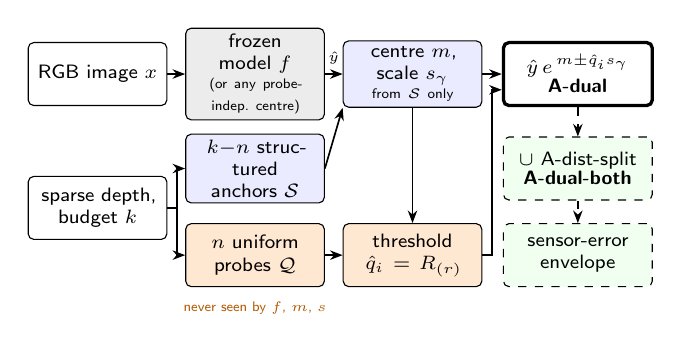
\begin{tikzpicture}[
  font=\sffamily\scriptsize,
  box/.style={draw, rounded corners=2pt, align=center, text width=1.62cm, minimum height=8mm, inner sep=2pt, fill=white},
  frozen/.style={box, fill=gray!15},
  anch/.style={box, fill=blue!8},
  prob/.style={box, fill=orange!18},
  outbox/.style={box, text width=1.75cm, fill=white, very thick},
  opt/.style={box, text width=1.75cm, dashed, fill=green!6},
  arr/.style={-{Stealth[length=1.6mm]}, semithick},
  darr/.style={-{Stealth[length=1.6mm]}, semithick, dashed}]
  % column 1: inputs
  \node[box]    (rgb)    at (0.85, 2.15) {RGB image $x$};
  \node[box]    (sensor) at (0.85, 0.45) {sparse depth,\\budget $k$};
  % column 2: model and split
  \node[frozen] (f)      at (2.85, 2.15) {frozen model $f$\\[-1pt]{\tiny(or any probe-indep.\ centre)}};
  \node[anch]   (S)      at (2.85, 0.95) {$k{-}n$ structured\\anchors $\cS$};
  \node[prob]   (Q)      at (2.85,-0.15) {$n$ uniform\\probes $\cQ$};
  % column 3: centre/scale and threshold
  \node[anch]   (ms)     at (4.85, 2.15) {centre $m$, scale $s_\gamma$\\[-1pt]{\tiny from $\cS$ only}};
  \node[prob]   (q)      at (4.85,-0.15) {threshold\\$\qhat_i=R_{(r)}$};
  % column 4: output and optional stages
  \node[outbox] (int)    at (6.95, 2.15) {$\yhat\,e^{\,m\pm\qhat_i s_\gamma}$\\[-1pt]\textbf{\mDual}};
  \node[opt]    (hull)   at (6.95, 0.95) {$\cup$ \mDistSplit\\[-1pt]\textbf{\mDualBoth}};
  \node[opt]    (env)    at (6.95,-0.15) {sensor-error\\envelope};
  % arrows
  \draw[arr] (rgb) -- (f);
  \draw[arr] (f) -- node[above, font=\tiny\sffamily]{$\yhat$} (ms);
  \draw[arr] (sensor.east) -- ++(0.12,0) |- (S.west);
  \draw[arr] (sensor.east) -- ++(0.12,0) |- (Q.west);
  \draw[arr] (S.east) -- (ms.south west);
  \draw[arr] (Q) -- (q);
  \draw[arr] (ms) -- (q);
  \draw[arr] (ms) -- (int);
  \draw[arr] (q.east) -- ++(0.12,0) |- ([yshift=-2mm]int.west);
  \draw[darr] (int) -- (hull);
  \draw[darr] (hull) -- (env);
  \node[font=\tiny\sffamily, text=orange!70!black, anchor=north] at (2.85,-0.62) {never seen by $f$, $m$, $s$};
\end{tikzpicture}
\caption{\textbf{Dual-role calibration.} Structured anchors $\cS$ build a centre $m$ and scale $s_\gamma$ around a frozen prediction $\yhat$ (or any probe-independent centre); the $n$ uniform probes $\cQ$ only score it and set one threshold per image (\cref{thm:dual}). Dashed: optional stages (\ifenvelopemain\cref{thm:both,prop:env}\else\cref{thm:both}; Supp.~D\fi).}
\label{fig:pipeline}
\end{figure}


\paragraph{Architecture (\cref{fig:pipeline}).}
(1)~A frozen monocular model produces $\yhat$.
(2)~The sensor budget is split into $k-n$ anchors $\cS$ that follow the deployed layout and $n$ uniformly random probes $\cQ$.
(3)~The anchors alone build a local centre $m(p)$ and scale $s(p)$ around $\yhat$ with the \mDist model of \cref{eq:scale}, fitted on $\cS$ only.
(4)~The probes, unseen by stages 1--3, set one conformal threshold per image.
Stage~1 can be any predictor that does not see the probes, \eg a depth-completion network fed RGB and $\cS$; stage~3 is then refit around its output.
\mDual is therefore a calibration layer, not a depth estimator.

\paragraph{Scale shrinkage.}
When the anchors set the shift wrong everywhere, as a single cluster can, the residual is nearly flat.
The threshold is then set by the probes with the smallest $s$, and widths elsewhere grow by up to $\max s/\min s$.
We therefore shrink the scale toward its per-image median $M_i=\med_{p\in\cP_i}s(p)$:
\begin{equation}
s_\gamma(p)=M_i\big(s(p)/M_i\big)^{\gamma},\qquad\gamma=0.5.
\label{eq:shrink}
\end{equation}

\paragraph{Per-image threshold.}
For probes $\cQ=\{p_1,\dots,p_n\}$ with reported residuals $\dtil(p_j)$,
\begin{equation}
R_j=\frac{|\dtil(p_j)-m(p_j)|}{s_\gamma(p_j)},\qquad\qhat_i=R_{(r)},\qquad r=\lceil(n+1)(1-\alpha)\rceil,
\label{eq:threshold}
\end{equation}
where $R_{(r)}$ is the $r$-th smallest score ($\qhat_i=\infty$ if $r>n$).
The interval at every evaluation pixel is
\begin{equation}
C(p)=\Big[\yhat(p)\,e^{\,m(p)-\qhat_i s_\gamma(p)},\;\yhat(p)\,e^{\,m(p)+\qhat_i s_\gamma(p)}\Big].
\label{eq:interval}
\end{equation}

\begin{theorem}[Dual-role validity]
\label{thm:dual}
Fix an image with valid pixels $\cP$ and a structured anchor set $\cS\subset\cP$ chosen by any rule, which may depend on $x$, $\yhat$ and the anchor values.
Let $m$, $s>0$ and $\gamma$ be determined by $(x,\yhat,\cS,\dtil|_\cS)$.
Let $v$ be the log residual of the quantity the probes report ($v=d$ for exact depth, $v=\dtil$ for a sensor).
Draw $\cQ$ uniformly without replacement from $\cU=\cP\setminus\cS$, compute $\qhat$ by \cref{eq:threshold} with $v$, and let $J$ be uniform on $\cU\setminus\cQ$.
Then
\begin{equation*}
\P\big(\yhat(J)e^{v(J)}\in C(J)\,\big|\,x,\cS,\dtil|_\cS\big)\;\ge\;\frac{r}{n+1}\;\ge\;1-\alpha,
\end{equation*}
with equality on the left when the scores have no ties and $r\le n$.
Equivalently, $\E[\Cov_i\mid x,\cS]\ge r/(n+1)$, the expectation being over the probe draw.
\end{theorem}

\noindent\emph{Proof idea.}
Given the anchors, every pixel of $\cU$ carries a fixed score.
The probes together with $J$ form a uniformly random $(n+1)$-subset of $\cU$, so $J$'s score is among the $r$ smallest of the $n+1$ scores, and hence covered, with probability at least $r/(n+1)$.
The full proof is in \cref{app:proof-dual}. \hfill$\square$

The theorem needs no calibration images and uses all $n$ probes for the threshold; $n\ge9$ suffices at $\alpha=0.1$.
By contrast, \mLocalSplit, which applies \mLocal to the $n$ probes, spends half of them on a shift.
\emph{Scope:} the guarantee holds in expectation over the probe draw, not per region.
Probes must be uniform over the pixels it concerns.
Every choice, $\gamma$ included, must be fixed without looking at probe values.
And it covers $v$, the quantity the probes measure.

\paragraph{Probe budget.}
\Cref{thm:dual} fixes the mean of $\Cov_i$; the number of probes fixes its spread.

\begin{proposition}[Per-image coverage law]
\label{prop:budget}
Under \cref{thm:dual} with no ties and $r\le n$, let $N=|\cU|$.
The number of covered evaluation pixels, $(N-n)\Cov_i$, follows exactly the beta-binomial law $\BetaBin(N-n,\,r,\,n+1-r)$.
As $N\to\infty$, $\Cov_i\to\BetaD(r,\,n+1-r)$ in distribution.
\end{proposition}

This is the finite-population form of the Beta law of split-conformal coverage conditional on the calibration set~\cite{vovk2012conditional}; the proof is in \cref{app:proof-budget}.
It turns the probe count into a design parameter (\cref{tab:budget}).
The share of images below coverage $c$ in one draw, $\P(\BetaD(r,n{+}1{-}r)<c)$, is known before any data are seen.
At $\alpha=0.1$ it falls slowly with $n$ (\NumRuleShortHundred\% below 0.85 at $n=100$).
The nominal level is the stronger lever: $r=n=20$ (the \mDualRmax arm, nominal \NumRuleNomTwentyAll) leaves only \NumRuleShortTwentyAll\% of images below 0.85, at a width cost the confirmatory run measures (\pending{measured, $r=n$ arm}).

\begin{table}[t]
\centering\small
\caption{\textbf{Probe budget at $\alpha=0.1$, one probe draw}, from the Beta law of \cref{prop:budget} alone (no data).}
\label{tab:budget}
\begin{tabular}{@{}rrccc@{}}
\toprule
$n$ & $r$ & $r/(n+1)$ & 10th percentile of $\Cov_i$ & $\P(\Cov_i<0.85)$, \% \\
\midrule
10 & 10 & 0.909 & \NumBetaPTenTen   & \NumBetaShortOneTen \\
20 & 19 & 0.905 & \NumBetaPTenTwenty & \NumBetaShortOneTwenty \\
40 & 37 & 0.902 & \NumBetaPTenForty & \NumBetaShortOneForty \\
\bottomrule
\end{tabular}
\end{table}

\paragraph{A per-distance-bin guarantee (\mDualBoth).}
\mDual's coverage, in practice, decreases with the distance to the nearest anchor; \cref{thm:dual} allows this because it is an average over the image.
\mDistSplit (\cref{sec:method:anchors}, fitted on all $k$ measurements) has the opposite profile: a per-bin guarantee averaged over scenes, no per-image guarantee, and a need for calibration scenes with dense depth from the same source as the measurements.
\mDualBoth is the pointwise hull
$C^{\text{both}}(p)=\big[\min(\ell^{\text{dual}},\ell^{\text{dist}}),\,\max(u^{\text{dual}},u^{\text{dist}})\big]$.

\begin{theorem}[Hull validity]
\label{thm:both}
\mDualBoth has the per-image guarantee of \cref{thm:dual} and the per-bin guarantee of \mDistSplit.
\end{theorem}

\noindent\emph{Proof idea.} The hull contains each interval pointwise and both statements are monotone in the interval~\cite{gasparin2024merging} (\cref{app:proof-both}). \hfill$\square$

\noindent The broad study's \mDistBoth, the hull of \mDistSplit with \mLocalSplit, is the baseline that \mDualBoth replaces.
Any hull costs width, most when its two centres disagree, as under clustered anchors.

\subsection{Sensor-error envelope}
\label{sec:env}
With sensor-valued probes, \cref{thm:dual} certifies the reading $\ytil$, not the depth $y$.
Let $e=\log\ytil-\log y$ and suppose a reference (here a laser scan) exists on calibration scenes.
We (a)~subtract a global bias $\hat\beta$, the median of $e$ on head-train pixels, from the probe values.
We (b)~give each sensor-confidence class $c$ (ARKit: $0,1,2$) the band $[-a_c,b_c]=[Q_c(\lambda/2),Q_c(1-\lambda/2)]$ of the corrected head-train error, clipped to contain 0.
One conformal risk control over the $U$ calibration scenes sets $\hat\lambda$: the largest value on a fixed grid with $\frac{U}{U+1}\hat L(\lambda)+\frac{1}{U+1}\le\alpha_e$, where $\hat L$ is the mean fraction of a scene's pixels outside their band.
With $[\ell,u]$ the \mDual interval for the corrected reading at level $1-\alpha_s$, the enveloped interval (\mDualEnv) is
\begin{equation}
C^{\text{env}}(p)=\big[\ell(p)\,e^{-b_{c(p)}},\;u(p)\,e^{a_{c(p)}}\big].
\label{eq:envelope}
\end{equation}

\begin{proposition}[Envelope]
\label{prop:env}
If the sensor reading and its confidence are defined at every evaluation pixel, the miscoverage of $y$ by $C^{\text{env}}$, averaged over test scenes and probe draws, is at most $\alpha_s+\alpha_e$.
\end{proposition}

\noindent\emph{Proof idea.} $y$ can be missed only if the corrected reading falls outside $[\ell,u]$ (at most $\alpha_s$ per image, \cref{thm:dual}) or the corrected error falls outside its band (at most $\alpha_e$ in expectation, by risk control); a union bound concludes (\cref{app:proof-env}). \hfill$\square$

\noindent The per-image guarantee on $y$ is not retained, since the envelope part holds on average over scenes.
We fixed $\alpha_s=\alpha_e=0.05$ before the run.
One risk control over a single class-adaptive parameter replaces per-class thresholds, which would all be infinite with 37 calibration scenes (\cref{app:proof-env}); this design was amended before any envelope output existed.


\section{Experiments and Results}
\label{sec:experiments}

\subsection{Datasets, models and protocol}
\label{sec:protocol}

\paragraph{Datasets.}
\Cref{tab:data} in \cref{app:data} lists the five datasets.
NYU Depth v2~\cite{silberman2012nyu} and KITTI~\cite{geiger2012kitti} are used throughout; on KITTI the ground truth is built from the same LiDAR that would provide anchors, so it cannot test an independent sensor.
DIODE~\cite{vasiljevic2019diode} and ETH3D~\cite{schops2017eth3d} test domain shift and the case of very few scenes.
ARKitScenes~\cite{baruch2021arkitscenes} (depth-upsampling validation split) provides an independent sensor.
Its ground truth is a Faro laser scan, while the deployed sensor is the iPad Pro LiDAR depth from ARKit (fused, with confidence classes $0,1,2$), which reads about \NumArkIpadOffset\% nearer than the laser.
Valid pixels are kept on a regular lattice (stride 4 on NYU, 2 on KITTI and DIODE, 8 on ARKitScenes) and stored per image, so per-image statistics are exact.
Every split is by scene: head-train (fits scores, $m$, $s$ and hyper-parameters), calibration (cross-scene thresholds; unused by \mDual) and test.
The main-method experiments use 30/35/35\%.


\paragraph{Frozen models.}
We use UniDepthV2-Large~\cite{piccinelli2025unidepthv2}, Depth Anything V2 Large metric~\cite{yang2024dav2} (indoor checkpoint on NYU, DIODE indoor and ARKitScenes; outdoor checkpoint on KITTI and DIODE outdoor), Depth Pro~\cite{bochkovskii2025depthpro} and Metric3D v2 ViT-Large~\cite{hu2024metric3dv2}.
Metric3D v2 is given the calibrated focal length, while the other three infer the camera, so it is not compared like for like.
NYU and KITTI are not in the training mixtures of these models.
UniDepthV2's training mixture includes ARKitScenes, which can affect width but not any guarantee; Depth Pro was trained on ARKitScenes and is not used there.
On ARKitScenes we also use the depth-completion network \omnidc~\cite{zuo2025omnidc} (v1.1, trained only on synthetic data).
It sees RGB and the structured anchors only, never the probes.
\Cref{fig:models} shows the ARKitScenes inputs and the two frozen models used there.

\begin{figure}[t]
\centering
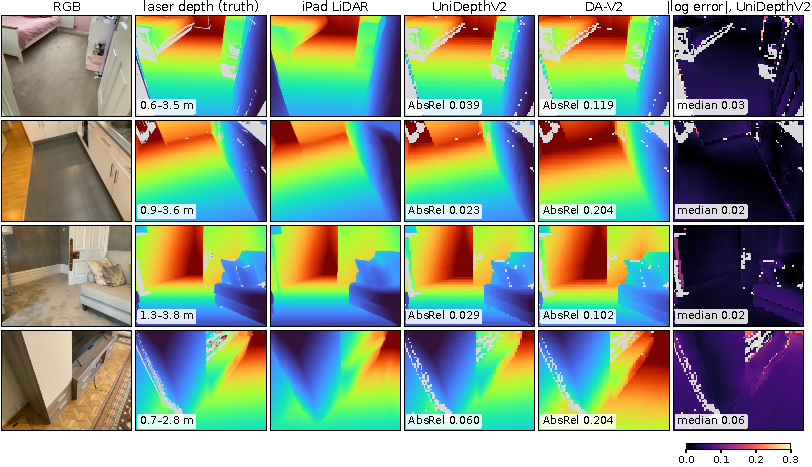
\includegraphics[width=\linewidth]{figures/models_qual.pdf}
\caption{\textbf{ARKitScenes: the reference, the deployed sensor and two frozen models} (four frames from different homes, chosen for their depth range, so their errors are below the dataset average of AbsRel \NumArkUniAbsRel{} for UniDepthV2 and \NumArkDavAbsRel{} for DA-V2). Depth panels of a row share one colour scale (range in the laser panel; grey: no value). The laser scan is the ground truth; the iPad LiDAR is smooth and reads slightly nearer. Predictions and the error map are shown on the evaluation lattice (stride 8). DA-V2 (indoor metric) overestimates depth throughout, the global scale error that anchors remove.}
\label{fig:models}
\end{figure}

\paragraph{Metrics.}
Coverage is image-averaged (\cref{eq:cov}).
Per-image spread is the 10th percentile (p10) of $\Cov_i$ and the share of \emph{short} images, whose coverage on one probe draw is below $1-\alpha-0.05=0.85$ (theory at $n=20$: \NumBetaShortOneTwenty\%).
Width is the median relative width; IS is the relative interval score of \cref{sec:problem}.
$\alpha=0.1$ unless stated.

\paragraph{Protocol and decision rules.}
The broad study used 20 random scene splits for the cross-image calibrators and 3--5 splits $\times$ 2--6 anchor draws for the anchor experiments.
A method was called \emph{valid} if its mean coverage over splits is at least $1-\alpha-2\,$SE.
It was called \emph{better} than another only if the 95\% paired bootstrap interval of their interval-score difference over splits excludes zero.
The dual-anchor experiments were first run in an exploratory phase (3 splits $\times$ 2 probe draws), which chose the shrinkage $\gamma=0.5$ after $\gamma=1$ showed a heavy width tail.
All comparisons are then replicated in a confirmatory run whose analysis plan was frozen before the runs: E17c (\NumReplSplits{} splits $\times$ \NumProbeDraws{} probe draws on NYU and KITTI, plus an $r=n$ arm), E18c (the same on ARKitScenes), E19c (10 visit splits, each with its own anchor mask) and E20 (the envelope).
The plan also fixes two thresholds in advance.
The completion centre ``wins'' a layout only if its best valid method beats UniDepthV2 $+$ \mDual by at least 15\% in IS.
The envelope enters the main method only if its truth coverage is valid and it beats \mDistBoth by at least 10\%.
Two amendments were logged before any affected output was seen: the primary IS definition, and the single-CRC envelope of \cref{sec:env}.

\subsection{Broad study: what conformal wrapping and anchors can and cannot do}
\label{sec:res:broad}

\Cref{tab:broad} summarizes the broad study; details and further tables are in \cref{app:broad}.

\begin{table}[t]
\centering\small
\caption{\textbf{Broad study (E0--E16), headline results.} Plain log score, $\alpha=0.1$; ranges over the NYU/KITTI $\times$ model pairs unless stated. The E13 row is re-measured by the confirmatory run (E17c).}
\label{tab:broad}
\footnotesize
\setlength{\tabcolsep}{3pt}
\begin{tabular}{@{}p{0.2\linewidth}p{0.77\linewidth}@{}}
\toprule
Experiment & Result \\
\midrule
E0 accuracy & AbsRel on NYU / KITTI: UniDepthV2 0.071 / 0.077, DA-V2 0.206 / 0.109, Depth Pro 0.092 / 0.139, Metric3D v2 0.066 / 0.048. \\
E2--E4 validity & Cross-image CRC (K1) covers 0.894--0.900 on every NYU/KITTI pair; raw uncertainties claiming 90\% cover 3--16\% (flip), 15--43\% (ensemble) and 83--91\% (learned variance). \\
E1, E8 units & Run-to-run SD of coverage follows the Beta law with $n=$ \#images and is ${\approx}100\times$ the pixel-count prediction (\cref{fig:units}). \\
Scene level & Image-event calibration is slightly short on scene-clustered data (0.884--0.897); its scene version meets the target (0.908--0.940) for 3--12\% more width. \\
E5 shift, ETH3D & Calibrating on one dataset and testing on another: 33--85\% coverage. On ETH3D (13 scenes) a scene-dependent scale bias drops Depth Pro to 0.69; scene-level calibration needs $\ge9$ calibration scenes and returns infinite intervals with 4. \\
E11 anchors & One global scale error explains \NumScaleVarLo--\NumScaleVarHi\% of image-to-image variation in coverage. About 20 random anchors match an oracle that knows each image's scale, giving intervals 1.1--3.7$\times$ narrower. \mLocal matches its exact theory (0.908--0.910 vs.\ 0.909 at $k=20$), and \mBoth cuts short images from 16\% to 0.2\% (NYU, DA-V2). \\
E13 structured & \mLocal on structured anchors covers \ESeventeen{cluster}{50}{local}/\ESeventeen{cluster}{200}{local} (cluster), \ESeventeen{near}{50}{local}/\ESeventeen{near}{200}{local} (near), \ESeventeen{rows}{50}{local}/\ESeventeen{rows}{200}{local} (rows; $k=50/200$, median over pairs, E17c), with \emph{narrower} intervals. Cross-image \mRescale and \mHybrid stay valid under every layout. \\
E14 \mDist & Coverage is flat across distance to the nearest anchor under all five layouts, and up to 67\% narrower than \mHybrid. With 20 of the $k$ anchors spent at random, \mDistBoth covers 0.965--0.983 with $\le$0.3\% short images. \\
E15 mismatch & Calibrating under one layout and deploying another leaves coverage as low as 0.77 (\mHybrid, edges $\to$ cluster). The largest threshold over layouts (@max) is valid for each layout. LSCP covers 0.17--0.93, depending on the layout. \\
E16 noise & With matched sensor noise, every cross-image guarantee holds (0.916--0.925). Calibrating on clean anchors fails under outliers (\mDist 0.66) and a 5\% bias (0.36--0.86). Within-image methods cover the sensor reading, so a bias breaks them (0.38--0.78). \\
E12 safety & Only guarantees calibrated on the query itself (nearest depth in a region) are valid and informative. Per-pixel guarantees leave the region minimum over-estimated in 2--24\% of images, and simultaneous coverage of all pixels raises alarms on 99--100\% of safe images. \\
\bottomrule
\end{tabular}
\end{table}

\begin{figure}[t]
\centering
\begin{minipage}[t]{0.47\linewidth}
\centering
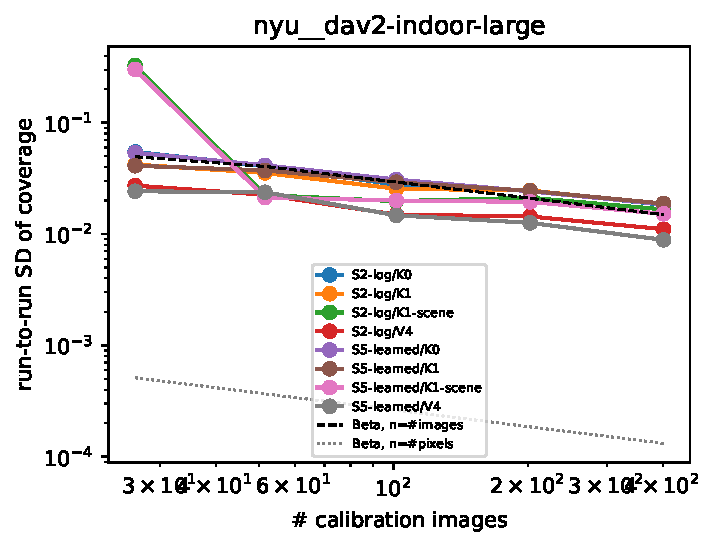
\includegraphics[width=\linewidth]{e8_calsize__nyu__dav2-indoor-large.pdf}
\captionof{figure}{\textbf{The image is the unit (E8, NYU, DA-V2).} Run-to-run SD of coverage against the number of calibration images (50 splits). Dashed: Beta law with $n=$ \#images; dotted: with $n=$ \#pixels.}
\label{fig:units}
\end{minipage}\hfill
\begin{minipage}[t]{0.49\linewidth}
\footnotesize
\textbf{Reading the findings.}
Conformal wrapping fixes \emph{average} coverage everywhere at modest cost, and the score matters: learned or relative scores give up to 20\% lower interval score.
What cross-image calibration cannot fix is the spread of coverage across individual images (16\% of NYU images short with DA-V2), or a change of dataset without target calibration data.
Anchors attack the dominant per-image error, the global scale.
Within-image calibration then gives a per-image guarantee that needs no calibration set at all (on DIODE it is the only finite option: 0.900 coverage at $k=200$).
But it holds only for random anchors, and every failure under structured anchors is \emph{silent}: the intervals look tighter, not looser.
\end{minipage}
\end{figure}

\paragraph{Pixels are not the unit (Q1).}
On synthetic data with a controllable per-image scale error, average coverage stays at 0.90 while the spread of per-image coverage grows from 0.006 to 0.195: average validity says nothing about individual images.
On real data the run-to-run variability tracks the image-count prediction within a factor of 0.8--1.7 (\cref{fig:units}).
With few, very different scenes (ETH3D, 4 calibration scenes per split) the small slip of image-level guarantees becomes a collapse, and the valid scene-level version is uninformative.

\paragraph{Structured anchors break within-image calibration (Q2).}
Cross-image anchor methods stay valid under every layout, because calibration and test share it, at a width cost (clustered anchors make \mHybrid 26--61\% wider than random anchors at $k=20$).
\mLocal fails, and with it \mBoth's per-image guarantee: under clustered or near-only anchors 5--14\% of \mBoth's images fall below 0.80, against 0.3--2\% with random anchors.
Coverage also falls with distance to the nearest anchor even for random anchors, from \NumLocalNearBinCovLo--\NumLocalNearBinCovHi{} next to an anchor to \NumLocalFarBinCovLo--\NumLocalFarBinCovHi{} at 0.1--0.2 of the image diagonal.

\begin{figure}[t]
\centering
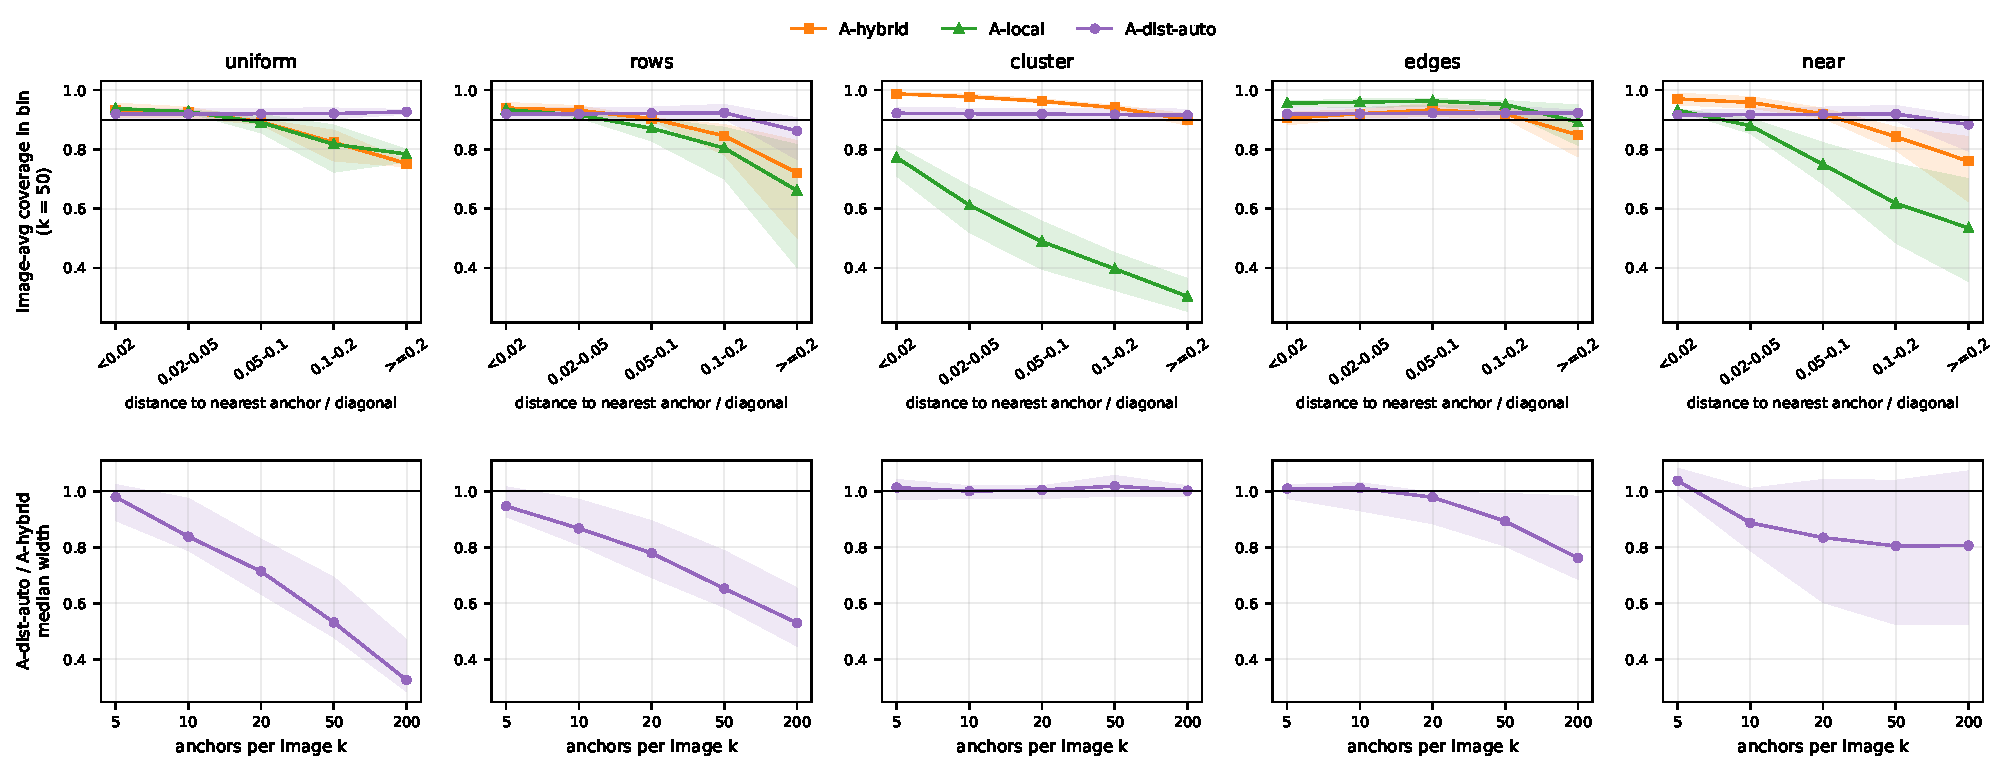
\includegraphics[width=0.9\linewidth]{e14_distance__S2-log.pdf}
\caption{\textbf{Distance-aware anchors (E14).} Top: image-averaged coverage per bin of distance to the nearest anchor ($k=50$; mean over the six NYU/KITTI pairs, band: min--max; line: 0.9). \mLocal collapses with distance under structured layouts; \mDist stays flat under all five. Bottom: \mDist's median width relative to \mHybrid against the number of anchors.}
\label{fig:adist}
\end{figure}

\paragraph{The distance-aware model and its limits.}
\mDist removes the distance gradient (\cref{fig:adist}).
At $k=20$ under uniform anchors its farthest-bin coverage is 0.86--0.91, where \mHybrid's is 0.66--0.83.
It is narrower wherever the anchors spread over the image (uniform: $-29\%$ at $k=20$, $-67\%$ at $k=200$; rows: up to $-47\%$) and within 6\% of \mHybrid under clusters.
Its guarantee is still an average over scenes, and it inherits two weaknesses of cross-image calibration.
Under a layout mismatch it misses by up to 4 points on average (0.863, near $\to$ edges); @max calibration fixes this at a width cost.
With noisy anchors, calibrating on clean data is unsafe: with 10\% outliers it covers 0.66 at $k=200$, and next to the anchors only 0.63.
Spending 20 measurements at random and taking the hull with \mLocalSplit (\mDistBoth) restores a per-image guarantee under every layout.
This budget split is the seed of the main method: the random measurements do the calibrating, so the structured ones need not.

\subsection{Main method: structured anchors break reused calibration; probes restore it}
\label{sec:res:failure}
\label{sec:res:dual}

\begin{table}[t]
\centering\footnotesize
\caption{\textbf{NYU and KITTI, three frozen models (UniDepthV2, DA-V2, Depth Pro), $n=20$ probes, $\alpha=0.1$} (confirmatory E17c, \NumReplSplits{} scene splits $\times$ \NumProbeDraws{} probe draws); median over the six model--dataset pairs. \textsf{local}: \mLocal calibrated on the $k$ structured anchors themselves; \textsf{dual}: \mDual; \textsf{both}: \mDualBoth. Short: \% of images whose coverage on one probe draw is below 0.85. $\Delta$: change in median relative width and relative IS (primary) against \mDistBoth. $^\dagger$Uniform anchors only. $^\ddagger$\Cref{tab:budget}.}
\label{tab:main}
\setlength{\tabcolsep}{4pt}
\newcommand{\rowE}[3]{#1 & #3 & \ESeventeen{#2}{#3}{local} & \ESeventeen{#2}{#3}{dual} & \ESeventeen{#2}{#3}{short} & \ESeventeen{#2}{#3}{dW} & \ESeventeen{#2}{#3}{bW} & \ESeventeen{#2}{#3}{dIS} & \ESeventeen{#2}{#3}{bIS} \\}
\begin{tabular}{@{}llccccccc@{}}
\toprule
 & & \multicolumn{2}{c}{Coverage} & Short (\%) & \multicolumn{2}{c}{$\Delta$ width (\%)} & \multicolumn{2}{c}{$\Delta$ IS (\%)} \\
\cmidrule(lr){3-4}\cmidrule(lr){5-5}\cmidrule(lr){6-7}\cmidrule(l){8-9}
Layout & $k$ & \textsf{local} & \textsf{dual} & \textsf{dual} & \textsf{dual} & \textsf{both} & \textsf{dual} & \textsf{both} \\
\midrule
\rowE{uniform}{uniform}{50}\rowE{}{uniform}{200}
\midrule
\rowE{rows}{rows}{50}\rowE{}{rows}{200}
\midrule
\rowE{cluster}{cluster}{50}\rowE{}{cluster}{200}
\midrule
\rowE{edges}{edges}{50}\rowE{}{edges}{200}
\midrule
\rowE{near}{near}{50}\rowE{}{near}{200}
\midrule
\multicolumn{2}{@{}l}{theory} & $\ge$0.9$^\dagger$ & \NumDualCovTheory & \NumBetaShortOneTwenty$^\ddagger$ & & & & \\
\bottomrule
\end{tabular}
\end{table}

\paragraph{Failure (\cref{tab:main}, \textsf{local}).}
Calibrating within the image on the structured anchors themselves keeps nominal coverage only for uniform anchors.
Under clustered anchors it covers \ESeventeen{cluster}{50}{local} and \ESeventeen{cluster}{200}{local} at $k=50$ and 200 (medians over the six pairs; range over pairs and both budgets \NumLocalClusterCovLo--\NumLocalClusterCovHi); under near-only anchors \ESeventeen{near}{50}{local} and \ESeventeen{near}{200}{local}; under scan lines \ESeventeen{rows}{200}{local} at $k=200$.
Edge anchors over-cover, since edges are where errors are largest.
The failing intervals are narrower, not wider: with 50 clustered anchors their median relative width is \NumLocalClusterWidthLo--\NumLocalClusterWidthHi, against \NumLocalUnifWidthLo--\NumLocalUnifWidthHi{} for uniform ones.
Even uniform anchors hide a spatial gap: at $k=50$, coverage falls from \NumLocalNearBinCovLo--\NumLocalNearBinCovHi{} within 0.02 of the image diagonal from an anchor to \NumLocalFarBinCovLo--\NumLocalFarBinCovHi{} at 0.1--0.2 of it.
\Cref{fig:layouts} shows both effects on one frame.

\begin{figure}[t]
\centering
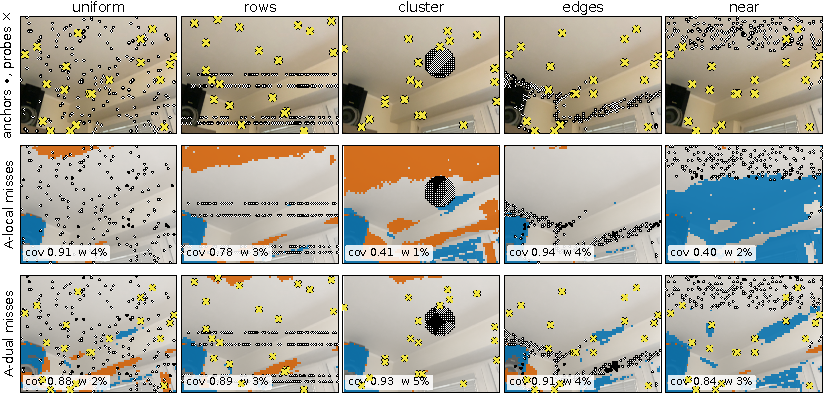
\includegraphics[width=\linewidth]{figures/layouts_qual.pdf}
\caption{\textbf{One ARKitScenes test frame under the five anchor layouts} (UniDepthV2, $k=200$: 180 structured anchors $\bullet$ and 20 probes $\times$, laser values, split 0, one draw). Rows 2--3: pixels whose true depth lies outside the interval (vermillion: truth farther, blue: nearer); cov: coverage of the frame's evaluation pixels; w: median relative width. \mLocal, calibrated on the structured anchors, holds only where they are representative: under clustered and near-only anchors it covers 0.41 and 0.40 with intervals 1--2\% wide. \mDual, calibrated on the probes, stays near 0.9 in every layout; its frame-to-frame spread around $0.905$ is the law of \cref{prop:budget}.}
\label{fig:layouts}
\end{figure}

\paragraph{Separating the roles restores per-image validity.}
\mDual covers \NumDualCovLo--\NumDualCovHi{} in every layout, $k$ and pair, at its theoretical rate $r/(n+1)=\NumDualCovTheory$ (within two standard errors in \NumDualExactCells{} of the \NumAllCells{} pair--layout--$k$ cells).
It is at least 10\% narrower than the hull baseline \mDistBoth on \NumDualGatePairs{} of \NumPairs{} pairs in each of the \NumCells{} layout--$k$ cells, and \NumDualWidthGainLo--\NumDualWidthGainHi\% narrower overall (median over pairs; paired bootstrap intervals exclude 0).
Part of that width is \mDistBoth's over-coverage (\NumDistBothCovLo--\NumDistBothCovHi), so the interval score, which charges misses, is the fairer comparison.
On it \mDual is better in \NumDualISWins{} of the \NumAllCells{} cells, including every cell with uniform or scan-line anchors (by \NumDualISGainURLo--\NumDualISGainURHi\%); \mDistBoth is better in \NumDualISLosses, nine of them clustered, by at most \NumDualISLoseMax\%.
\mDualBoth is better than \mDistBoth in \NumDualBothISWins{} cells and worse in \NumDualBothISLosses, all clustered and by at most \NumDualBothISLoseMax\%.
Under clustered anchors its two halves are centred differently and it gains only \NumDualBothClusterWidthLo--\NumDualBothClusterWidthHi\% in width.
\mDual's coverage varies across distance bins by \NumSpreadDualLo--\NumSpreadDualHi{} points; \mDualBoth reduces this to \NumSpreadDualBothLo--\NumSpreadDualBothHi{} (\cref{fig:dual}a).

\begin{figure}[t]
\centering
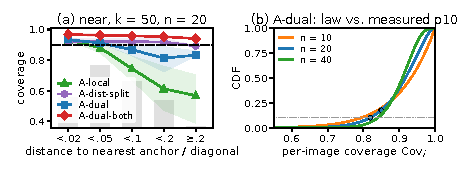
\includegraphics[width=0.8\linewidth]{figures/e17_results.pdf}
\caption{\textbf{What each guarantee protects (E17).} (a)~Near layout, $k=50$, $n=20$: \mDual's coverage decreases with distance, as \cref{thm:dual} allows; \mDualBoth is flat. Lines/bands: median/range over the six NYU/KITTI pairs; bars: pixel share; dashed: 0.9. (b)~CDF of the per-image coverage law (\cref{prop:budget}) for $n=10,20,40$ (theory); dots, $n=20$: measured p10 of $\Cov_i$ at 0.1 and measured share of short images at 0.85 (median over pairs, layouts and $k$; bars: range).}
\label{fig:dual}
\end{figure}

\paragraph{The probe budget.}
With 20 probes the 10th percentile of $\Cov_i$ was \NumMeasPTenTwenty{} (law: \NumBetaPTenTwenty), an implementation check of the randomization (\cref{fig:dual}b).
With 10 probes \mDistBoth is infinite on every image by construction; 40 probes tighten the law only slowly at twice the measurement cost, so we keep $n=20$ (\cref{app:budget}).

\subsection{Which centre to calibrate: a depth-completion network or the frozen model (E19c)}
\label{sec:res:omni}

\begin{table}[t]
\centering\footnotesize
\caption{\textbf{ARKitScenes, which centre to calibrate (E19c, confirmatory).} $k=200$ (180 structured anchors $+$ 20 probes), laser-valued anchors and probes, $\alpha=0.1$; mean over ten visit splits, one probe draw each. UniDepthV2 is frozen; \omnidc is completed from RGB and the 180 anchors. \mSplitCP calibrates one quantile on dense laser depth of calibration scenes; the UniDepthV2 \mSplitCP row uses no anchors. W$/y$: median width over laser depth; IS: primary relative interval score. Theory for \mDual, one draw: coverage \NumDualCovTheory, p10 \NumBetaPTenTwenty.}
\label{tab:omni}
\setlength{\tabcolsep}{3.5pt}
\newcommand{\eO}[3]{\ENineteen{#1}{#2}{clean}{clean}{#3}{cov} & \ENineteen{#1}{#2}{clean}{clean}{#3}{ptten} & \ENineteen{#1}{#2}{clean}{clean}{#3}{wgt} & \ENineteen{#1}{#2}{clean}{clean}{#3}{is}}
\newcommand{\rowO}[3]{#1 & #3 & \eO{uniform}{#2}{#3} & \eO{cluster}{#2}{#3} \\}
\begin{tabular}{@{}llcccc@{\hspace{8pt}}cccc@{}}
\toprule
 & & \multicolumn{4}{c}{Uniform layout} & \multicolumn{4}{c}{Cluster layout} \\
\cmidrule(lr){3-6}\cmidrule(l){7-10}
Centre & Calibration & Cov. & p10 & W$/y$ & IS & Cov. & p10 & W$/y$ & IS \\
\midrule
\rowO{UniDepthV2}{unidepth}{split-CP}
\midrule
\rowO{UniDepthV2 + $\cS$}{unidepth}{A-dist-split}
\rowO{}{unidepth}{A-dual}
\rowO{}{unidepth}{A-dual-both}
\midrule
\rowO{\omnidc + $\cS$}{omnidc}{split-CP}
\rowO{}{omnidc}{A-dist-split}
\rowO{}{omnidc}{A-dual}
\rowO{}{omnidc}{A-dual-both}
\bottomrule
\end{tabular}
\end{table}

\paragraph{Uniform anchors: the completion network is the better centre.}
\mSplitCP, \mDual and \mDistSplit on \omnidc's output have a \NumOmniGainLo--\NumOmniGainHi\% lower IS than \mDual on UniDepthV2 (\cref{tab:omni}; all paired intervals exclude zero).
This fires the pre-specified $\ge$15\% criterion, so the layer belongs on top of the completion network.
\mDual on \omnidc costs \NumOmniDualCost\% in IS over \mSplitCP on the same output and adds the per-image law: p10 \ENineteen{uniform}{omnidc}{clean}{clean}{A-dual}{ptten} and \ENineteen{uniform}{omnidc}{clean}{clean}{A-dual}{short}\% short images, as \cref{tab:budget} predicts.
\mSplitCP has no per-image guarantee and needs dense reference depth on calibration scenes.
Without anchors, \mSplitCP on the frozen model has \NumRawRatioLo--\NumRawRatioHi$\times$ the IS of any anchored method under uniform anchors, and 1.3--3.9$\times$ under clustered anchors.

\paragraph{Clustered anchors: the ranking reverses.}
Away from the one observed patch, the completion network extrapolates poorly.
\mSplitCP on its output is not valid (coverage \ENineteen{cluster}{omnidc}{clean}{clean}{split-CP}{cov}, more than 2\,SE below 0.9, p10 \ENineteen{cluster}{omnidc}{clean}{clean}{split-CP}{ptten}).
\mDual on UniDepthV2 has a \NumClusterGainDual\% lower IS than \mDual on \omnidc, and a \NumClusterGainCP\% lower IS than \mSplitCP on \omnidc.
On \omnidc itself, \mDual beats \mSplitCP by 17\%.
On the frozen centre, \mDistSplit is more efficient still (IS \ENineteen{cluster}{unidepth}{clean}{clean}{A-dist-split}{is}) but has no per-image guarantee, while \mDualBoth keeps both guarantees at \ENineteen{cluster}{unidepth}{clean}{clean}{A-dual-both}{is}.
Across both centres and layouts, \mDual's per-image spread is the same (p10 \NumENineteenPTenLo--\NumENineteenPTenHi, \NumENineteenShortLo--\NumENineteenShortHi\% short), as \cref{thm:dual} requires of any probe-independent centre.

\paragraph{Point accuracy agrees.}
On the test pixels outside the structured anchors (image-mean AbsRel, mean over the ten splits), \omnidc reaches 0.0064 under uniform and 0.0738 under clustered anchors.
UniDepthV2 rescaled per image by the median $\log(y/\yhat)$ at the same 180 anchors reaches 0.0293 and 0.0394, and 0.121 without anchors.
$\delta<1.25$ is 0.997 vs.\ 0.988 (uniform) and 0.944 vs.\ 0.981 (cluster).
So under uniform anchors \omnidc is about $4.6\times$ more accurate, while under clustered anchors a single per-image scale on the frozen model halves \omnidc's error.
This supports the interval-score result independently.
A mean-over-images IS would instead be dominated by a few \omnidc pixels with extreme upper bounds under clustered anchors (\cref{app:blowup}).

\subsection{What the probes certify: an independent sensor (E18)}
\label{sec:res:sensor}

\begin{table}[t]
\centering\footnotesize
\caption{\textbf{Laser-truth coverage by value source of anchors / probes} (ARKitScenes, $k=200$, $\alpha=0.1$; L $=$ laser, I $=$ iPad LiDAR). Frozen-model rows: confirmatory E18c, mean over \NumReplSplits{} visit splits and ten probe draws; \mDualEnv: E20, same splits and draws, iPad probes only. \omnidc rows: E19c, ten splits; \omnidc completed from iPad anchors (I/L, I/I) was not part of the confirmatory run (--).}
\label{tab:sensor}
\setlength{\tabcolsep}{4pt}
\newcommand{\eB}[3]{\ENineteen{#1}{#2}{clean}{clean}{#3}{cov} & -- & \ENineteen{#1}{#2}{clean}{lidar}{#3}{cov} & --}
\newcommand{\rowB}[3]{#1 & #3 & \eB{uniform}{#2}{#3} & \eB{cluster}{#2}{#3} \\}
\newcommand{\eC}[3]{\EEighteen{#1}{#2}{clean}{clean}{#3}{cov} & \EEighteen{#1}{#2}{lidar}{clean}{#3}{cov} & \EEighteen{#1}{#2}{clean}{lidar}{#3}{cov} & \EEighteen{#1}{#2}{lidar}{lidar}{#3}{cov}}
\newcommand{\rowC}[3]{#1 & #3 & \eC{uniform}{#2}{#3} & \eC{cluster}{#2}{#3} \\}
\newcommand{\eEnv}[2]{-- & -- & \ETwenty{#1}{#2}{clean}{A-dual-env}{cov} & \ETwenty{#1}{#2}{lidar}{A-dual-env}{cov}}
\newcommand{\rowEnv}[1]{ & \mDualEnv & \eEnv{uniform}{#1} & \eEnv{cluster}{#1} \\}
\begin{tabular}{@{}llcccc@{\hspace{10pt}}cccc@{}}
\toprule
 & & \multicolumn{4}{c}{Uniform layout} & \multicolumn{4}{c}{Cluster layout} \\
\cmidrule(lr){3-6}\cmidrule(l){7-10}
Centre & Calibration & L/L & I/L & L/I & I/I & L/L & I/L & L/I & I/I \\
\midrule
\rowC{UniDepthV2 + $\cS$}{unidepth}{A-dist-split}
\rowC{}{unidepth}{A-local-split}
\rowC{}{unidepth}{A-dual}
\rowC{}{unidepth}{A-dual-both}
\rowC{}{unidepth}{A-dist-both}
\rowEnv{unidepth}
\midrule
\rowC{DA-V2 + $\cS$}{dav2}{A-dist-split}
\rowC{}{dav2}{A-local-split}
\rowC{}{dav2}{A-dual}
\rowC{}{dav2}{A-dual-both}
\rowC{}{dav2}{A-dist-both}
\rowEnv{dav2}
\midrule
\rowB{\omnidc + $\cS$}{omnidc}{split-CP}
\rowB{}{omnidc}{A-dist-split}
\rowB{}{omnidc}{A-dual}
\bottomrule
\end{tabular}
\end{table}

\Cref{tab:sensor} varies what the measurements report, with coverage always measured against the laser.
With laser probes, \mDual's spread on ARKitScenes, over UniDepthV2 and DA-V2 (AbsRel \NumArkUniAbsRel{} and \NumArkDavAbsRel) and both layouts, is as predicted (p10 \NumEEighteenPTen, short \NumEEighteenShort).
This is a check on data that were not used to choose $\gamma$.
\begin{itemize}[leftmargin=*,itemsep=1pt,topsep=2pt]
\item \emph{iPad anchors, laser probes:} \mDual covers the laser truth at \NumEEighteenCovIL{} in both layouts, with the clean-value spread (p10 \NumEEighteenPTen), because the probes measure the truth and absorb the anchors' bias into the threshold.
\mDistSplit, calibrated on the values the measurements report, covers it at only \NumEEighteenDistIpad{} under uniform anchors with iPad anchors (either probe source).
\item \emph{Laser anchors, iPad probes:} \mDual over-covers (\NumEEighteenCovLI{} uniform), with \NumEEighteenWiden$\times$ wider intervals, as the iPad's own errors enter the threshold.
\item \emph{iPad values for both}, the deployed configuration without a reference: \mDual certifies the iPad reading.
Under uniform anchors its intervals are about as narrow as the \NumArkIpadOffset\% sensor bias, and it covers the laser truth at only \NumEEighteenCovII{} (p10 \NumEEighteenPTenII).
The wider cluster intervals absorb more (\NumEEighteenCovIICluster), and the hull \mDualBoth recovers the truth there (\NumEEighteenHullIICluster) but not under uniform anchors (\NumEEighteenHullII).
Calibration within the image behaves the same: \mLocalSplit covers the truth at \NumEEighteenLocalSplitLaserLo{} with laser probes and \NumEEighteenLocalSplitIpadLo--\NumEEighteenLocalSplitIpadHi{} with iPad probes, in both layouts.
\end{itemize}
\Cref{fig:sensor} shows why on three frames: the iPad reads a few per cent nearer than the laser over much of a frame, so probes that report the iPad calibrate intervals around the iPad's depth, and the laser truth falls beyond them.

\begin{figure}[t]
\centering
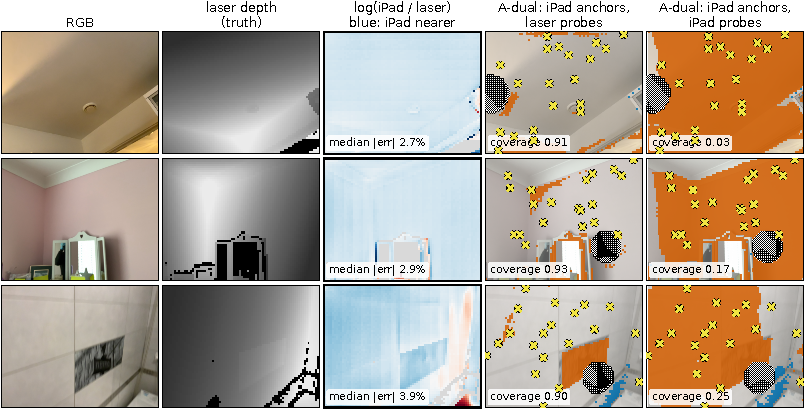
\includegraphics[width=\linewidth]{figures/sensor_qual.pdf}
\caption{\textbf{Probe source and truth coverage} (three ARKitScenes test frames from different visits; UniDepthV2, clustered layout, 180 structured anchors ($\bullet$, one cluster) reporting the iPad value, 20 probes ($\times$); split 0, one draw). Third column: log ratio of the iPad LiDAR to the laser depth (blue: iPad nearer; grey: no value). Right two columns: \mDual's misses of the laser truth (vermillion: truth farther than the interval, blue: nearer; dark grey: no ground truth), with laser and with iPad probes. Frames chosen among those whose coverage drops most from laser to iPad probes while staying near 0.9 with laser probes; averages over all frames are in \cref{tab:sensor}.}
\label{fig:sensor}
\end{figure}
Only \mDistBoth covers the truth in every cell of \cref{tab:sensor} (\EEighteen{uniform}{unidepth}{lidar}{lidar}{A-dist-both}{cov}--\EEighteen{uniform}{dav2}{clean}{clean}{A-dist-both}{cov}), and it does so through width, at \NumEEighteenDistBothRatio$\times$ \mDual's IS under uniform anchors with laser values (IS not shown).
\mSplitCP on \omnidc stays near nominal because it calibrates on laser depth of other scenes, which a deployed system lacks, but it is not valid under clustered anchors (\cref{sec:res:omni}).
Probes certify what they measure.

\paragraph{The sensor-error envelope (E20).}
The envelope of \cref{sec:env} restores truth coverage with iPad probes (\NumEnvTruthCov{} over both models, layouts and anchor sources), but it over-covers: its IS is \NumEnvISWorse{} above that of \mDistBoth (uniform \NumEnvISWorseUni, clustered \NumEnvISWorseCluster).
It therefore fails the gate fixed in advance (valid truth coverage and an IS at least 10\% below \mDistBoth) in both layouts, and \mDistBoth remains the cheaper way to cover the truth with sensor-grade probes.
The union bound behind \cref{prop:env} is loose here: \mDual at level $0.95$ already covers most of the truth, and widening every interval by the class band adds the rest again.

\section{Conclusions}
\label{sec:conclusions}

\paragraph{Findings.}
Conformal prediction turns frozen monocular metric depth models into per-pixel interval estimators with finite-sample guarantees, provided the guarantee is stated for the right unit: the image or the scene, not the pixel.
A cross-image guarantee is valid at modest cost, but it is an average that hides images with large global scale errors, and it does not survive a change of dataset.
A few sparse metric anchors remove most of the scale error (intervals 1.1--3.7$\times$ narrower).
Calibrating inside each image on its own anchors gives a per-image guarantee only for uniformly random anchors; under the layouts real sensors produce, it fails silently, with tighter intervals that miss most of the image.
Giving the sensor budget two roles fixes this.
Structured anchors build the prediction, and a few uniformly random probes, hidden from the predictor, calibrate it within each image.
The resulting layer needs no calibration images for validity (held-out images only tune its width), turns the probe count into a design parameter with a known per-image coverage law, and runs on any probe-independent centre.
A depth-completion network is the better centre under uniform anchors, and the frozen model with an anchor-built centre under clustered anchors (ten confirmatory splits, one network, one dataset).
Laser probes certified the depth even with iPad anchors; iPad probes certified only the iPad reading.

\paragraph{Limitations.}
\begin{itemize}[leftmargin=*,itemsep=1pt,topsep=2pt]
\item \emph{Expectation, not every draw:} with 20 probes about \NumBetaShortOneTwenty\% of images fall below 0.85 coverage in a single draw.
\item \emph{No spatial guarantee from probes alone:} the per-distance guarantee of \mDualBoth needs calibration scenes and the same anchor rule at deployment.
\item \emph{What is certified:} the probes' quantity.
The envelope that converts reading coverage into depth coverage holds only on average over scenes and, in our runs, costs more than \mDistBoth.
ARKit depth is fused and dense; raw sparse returns and dropouts on glass or sky are untested.
\item \emph{Selection of $\gamma$ and the design of \mDist} used NYU and KITTI, so only ARKitScenes checks efficiency on held-out data, and UniDepthV2 saw ARKitScenes in training.
\item \emph{Validity needs no images; efficiency does:} the \mDist variant, floor $\tau$ and distance function $g$ are chosen on 200 head-train images with dense ground truth under the same anchor layout. Without such images \cref{thm:dual} still holds, but the intervals may be wider.
\item \emph{Scope:} one $\alpha$ in the main method, two budgets, one independent sensor and uniform probes by design.
With a fixed-pattern scanner the guarantee covers only pixels with a return.
There is no downstream evaluation beyond the safety-query study.
\item \emph{Efficiency under clustered anchors:} there \mDual's interval score is up to \NumDualISLoseMax\% above the hull baseline's; its advantage is the per-image guarantee, not the score.
\end{itemize}

\paragraph{Future work.}
\begin{itemize}[leftmargin=*,itemsep=1pt,topsep=2pt]
\item A tighter sensor-error envelope that does not pay for both error sources separately.
\item Test raw, sparse sensor returns instead of fused depth, and video, where the probes could be shared across frames.
\item Study active placement of the anchors (the probes must stay random).
\item Evaluate the intervals inside a downstream AR or planning task, calibrating the guarantee to the query it protects, as the safety-query study suggests.
\end{itemize}


{\small
\bibliographystyle{plainnat}
\bibliography{../paper/refs,extra}
}

\appendix
\section{Proofs}
\label{app:proofs}

\subsection{Proof of \cref{thm:dual} (dual-role validity)}
\label{app:proof-dual}

\paragraph{Setting.}
Fix an image $x$ with its finite set $\cP$ of valid pixels, its prediction $\yhat$, a structured anchor set $\cS\subset\cP$ and the values $\dtil|_\cS$ reported at $\cS$.
Everything below is conditional on $(x,\yhat,\cS,\dtil|_\cS)$; since the statement holds for every realization, it also holds after averaging over any randomness in the layout.
By assumption, the centre $m$, the scale $s>0$, the per-image median $M=\med_{p\in\cP}s(p)$, and hence $s_\gamma=M(s/M)^\gamma$, are functions of $(x,\yhat,\cS,\dtil|_\cS)$, with $\gamma$ a fixed constant.
They are therefore fixed functions on $\cU=\cP\setminus\cS$.
Let $v:\cU\to\mathbb{R}$ be the log residual of the quantity the probes report.
Every $p\in\cU$ then carries a fixed score $R(p)=|v(p)-m(p)|/s_\gamma(p)$.
Let $N=|\cU|\ge n+1$ and $r=\lceil(n+1)(1-\alpha)\rceil$.

\paragraph{Coverage event.}
Since $s_\gamma>0$ and $\exp$ is increasing, $\yhat(p)e^{v(p)}\in C(p)$ if and only if $m(p)-\qhat s_\gamma(p)\le v(p)\le m(p)+\qhat s_\gamma(p)$, \ie if and only if $R(p)\le\qhat$.
For $v=d$, $\yhat e^{d}=y$, so this is coverage of the true depth.

\paragraph{Exchangeability.}
Let $(Z_1,\dots,Z_{n+1})$ be a uniformly random ordered sample without replacement from $\cU$, and set $\cQ=\{Z_1,\dots,Z_n\}$ and $J=Z_{n+1}$.
Then $\cQ$ is a uniform $n$-subset of $\cU$ and, given $\cQ$, $J$ is uniform on $\cU\setminus\cQ$, exactly as in the theorem.
The law of $(Z_1,\dots,Z_{n+1})$ is invariant under permutations and $R$ is a fixed function, so $(R(Z_1),\dots,R(Z_{n+1}))$ is exchangeable.

\paragraph{Rank argument.}
If $r>n$, $\qhat=\infty$ and coverage is 1.
Otherwise, break ties among the $n+1$ scores uniformly at random and let $\rho$ be the resulting rank of $R(Z_{n+1})$, which is uniform on $\{1,\dots,n+1\}$ by exchangeability.
If $\rho\le r$, at most $r-1$ of the $n$ probe scores are ranked below $R(Z_{n+1})$, so the $r$-th smallest probe score satisfies $\qhat\ge R(Z_{n+1})$.
Hence $\P(R(J)\le\qhat)\ge\P(\rho\le r)=r/(n+1)\ge1-\alpha$.
Without ties, $R(J)\le\qhat$ holds if and only if $\rho\le r$, so equality holds.

\paragraph{From one pixel to image coverage.}
Given $\cQ$, $J$ is uniform on $\cE=\cU\setminus\cQ$, so $\P(R(J)\le\qhat\mid\cQ)=\Cov_i$ (with $y$ replaced by $\yhat e^{v}$).
Taking expectations over $\cQ$ gives $\E[\Cov_i\mid x,\yhat,\cS,\dtil|_\cS]\ge r/(n+1)$. \hfill$\square$

\paragraph{Remarks.}
(a)~No assumption is made on how $\cS$ was chosen, on the distribution of images, or on $m$ and $s$ beyond their independence of the probe values.
This is why any layout and any probe-independent centre (\eg a completion network fed RGB and $\cS$) are allowed.
(b)~If any quantity used in $m$, $s$ or $\gamma$ were selected after looking at the probe values of the same image, $R$ would no longer be a fixed function and the argument would fail.
(c)~The probes must be uniform over the pixels the guarantee concerns; if a sensor cannot return at some pixels, $\cU$ and the guarantee are restricted to the pixels where it returns.
(d)~This is the split-conformal argument for a fitting set and a calibration set inside one instance~\cite{gui2023cmc}, and the within-field exchangeability argument~\cite{mao2024spatial}, specialized to a frozen prior and a structured fitting set.

\subsection{Proof of \cref{prop:budget} (per-image coverage law)}
\label{app:proof-budget}
Assume no ties among $\{R(p)\}_{p\in\cU}$ and $r\le n$.
Sort $\cU$ by score and let $T$ be the position of the $r$-th smallest probe, so $\qhat$ is the $T$-th smallest score in $\cU$.
Exactly $T-r$ non-probe pixels have score $\le\qhat$, so $(N-n)\Cov_i=T-r$.
For $T=r+j$, the sample must contain $r-1$ of the first $r+j-1$ pixels, the pixel at position $r+j$, and $n-r$ of the last $N-r-j$ pixels:
\begin{equation*}
\P(T-r=j)=\binom{r+j-1}{r-1}\binom{N-r-j}{n-r}\Big/\binom{N}{n},\qquad j=0,\dots,N-n.
\end{equation*}
This negative-hypergeometric law equals $\BetaBin(N-n,\,r,\,n+1-r)$, a standard identity (\eg via the P\'olya urn), which we also checked numerically to $10^{-14}$ for $N=300$, $n=20$.
Its mean is $(N-n)\,r/(n+1)$, so $\E[\Cov_i]=r/(n+1)$, the equality case of \cref{thm:dual}.
A beta-binomial variable is a binomial mixture with success probability $B\sim\BetaD(r,n+1-r)$.
Dividing by $N-n$ and letting $N\to\infty$ with $n$ fixed gives $\Cov_i\to B$ in distribution, the classical conditional-coverage law of split conformal prediction~\cite{vovk2012conditional}. \hfill$\square$

\noindent\emph{Numbers.} For $n=20$ ($r=19$): $\E[\Cov_i]=19/21=\NumDualCovTheory$, the 10th percentile is \NumBetaPTenTwenty, and $\P(\Cov_i<0.85)=\NumBetaShortOneTwenty\%$ for one draw.
With a few thousand evaluation pixels per image the finite-population correction is negligible at this precision.

\subsection{Proof of \cref{thm:both} (hull validity)}
\label{app:proof-both}
\paragraph{The per-bin guarantee of \mDistSplit.}
Let scenes be the exchangeable units.
The $U$ calibration scenes and one test scene are exchangeable, every image in them receives measurements by the same anchor rule, and all hyper-parameters of $m$ and $s$ are fitted on separate head-train scenes.
For a distance bin $b$ and threshold $\lambda$, let $L_{u,b}(\lambda)\in[0,1]$ be the average over the images of scene $u$ of the fraction of their bin-$b$ evaluation pixels with $|d-m|/s>\lambda$; it is non-increasing in $\lambda$.
Conformal risk control~\cite{angelopoulos2024crc} with $\hat\lambda_b=\inf\{\lambda:\frac{U_b}{U_b+1}\hat L_b(\lambda)+\frac{1}{U_b+1}\le\alpha\}$ gives $\E[L_{\text{test},b}(\hat\lambda_b)]\le\alpha$ for every bin (the Mondrian argument~\cite{vovk2005alrw}).
Bins supported by fewer than $2/\alpha-1$ calibration scenes are merged with the nearer neighbour, by a rule that depends on pixel positions only; the guarantee then holds for the merged bin.

\paragraph{Hull.}
For every evaluation pixel, $C^{\text{both}}(p)\supseteq C^{\text{dual}}(p)$ and $C^{\text{both}}(p)\supseteq C^{\text{dist}}(p)$.
So the hull's coverage indicator is at least the maximum of the two coverage indicators, pointwise.
Averaging over an image and taking the expectation over the probes gives \cref{thm:dual}'s bound.
Averaging over bin $b$ and taking the expectation over scenes gives the per-bin bound.
That \mDistSplit uses the probe values in its own fit is irrelevant to the first statement, which only uses the \mDual interval. \hfill$\square$

\subsection{Proof of \cref{prop:env} (envelope)}
\label{app:proof-env}
Let $e=\log\ytil-\log y$, $\hat\beta$ the bias estimated on head-train pixels, $\ytil'=\ytil e^{-\hat\beta}$ the corrected reading and $e'=e-\hat\beta$, so $y=\ytil'e^{-e'}$.
Run \mDual at level $1-\alpha_s$ with probes reporting $\ytil'$.
By \cref{thm:dual}, for every test image, the expected fraction of $\cE_i$ with $\ytil'\notin[\ell,u]$ is at most $\alpha_s$.
The bands $[-a_c(\lambda),b_c(\lambda)]$ are quantiles of $e'$ on head-train pixels only, so they form a fixed family that shrinks as $\lambda$ grows ($\lambda=0$: infinite bands).
Hence the loss $L_u(\lambda)$, the fraction of scene $u$'s pixels whose $e'$ lies outside the band of their class, lies in $[0,1]$, is non-decreasing in $\lambda$, and $L_u(0)=0$.
With exchangeable calibration and test scenes, conformal risk control (written for a loss that grows with $\lambda$) gives $\E[L_{\text{test}}(\hat\lambda)]\le\alpha_e$.
If $\ytil'(p)\in[\ell(p),u(p)]$ and $e'(p)\in[-a_{c(p)},b_{c(p)}]$, then $y(p)\in[\ell(p)e^{-b_{c(p)}},u(p)e^{a_{c(p)}}]=C^{\text{env}}(p)$.
So the fraction of a test scene's pixels that miss $y$ is at most the sum of the two failure fractions, whose expectations are at most $\alpha_s$ and $\alpha_e$. \hfill$\square$

\noindent\emph{Why one risk control.} Conformal risk control cannot certify a level below $1/(U+1)$, which is $0.026$ with $U=37$ calibration scenes per split.
Per-class one-sided targets proportional to the class shares (1.1, 4.3 and 94.6\% of pixels for confidence 0, 1, 2) would be $0.0003$, $0.001$ and $0.024$, and every threshold would be infinite.
A single two-sided risk control over one class-adaptive parameter avoids this; the grid has 400 log-spaced values in $[10^{-6},0.5]$.

\section{Which method gives which guarantee}
\label{app:notions}
\begin{table}[h]
\centering\small
\caption{\textbf{Guarantees at level $1-\alpha$.} ``Per image'' is in expectation over random anchors or probes and concerns the values they report. $^*$Per distance bin, averaged over scenes. $^\dagger$With a reference sensor; the depth guarantee is a scene average.}
\label{tab:notions}
\setlength{\tabcolsep}{4pt}
\begin{tabular}{@{}lllcc@{}}
\toprule
Method & Stage & Marginal unit & Per image & Per bin$^*$ \\
\midrule
K1, V4, K2, K3 (+ scene versions) & wrapper & image (scene) & -- & depth bins (K3) \\
\mRescale, \mHybrid & anchors & scene & -- & -- \\
\mLocal & anchors & -- & uniform anchors only & -- \\
\mBoth & anchors & scene & uniform anchors only & -- \\
\mDistSplit (\mDist) & anchors & scene & -- & yes \\
\mLocalSplit & dual & -- & yes & -- \\
\mDistBoth & dual & scene & yes & yes \\
\midrule
\mDual & dual & -- & yes, any layout & -- \\
\mDualBoth & dual & scene & yes, any layout & yes \\
\mDualEnv & dual & scene$^\dagger$ & sensor part only & -- \\
\mSplitCP (completion centre) & -- & scene & -- & -- \\
\bottomrule
\end{tabular}
\end{table}

\section{The distance-aware centre and scale}
\label{app:adist}
For pixel $p$, with anchor residuals $\dtil$ at the anchor set $\cA$ ($\cA=\cS$ for \mDual, all $k$ measurements for \mDistSplit):
\begin{itemize}[leftmargin=*,itemsep=1pt,topsep=2pt]
\item \textbf{Shift $m(p)$}, one of: \emph{median} (image median of $\dtil|_\cA$); \emph{knn} (median of the $K=16$ nearest anchors); \emph{kernel} (Gaussian-weighted mean of the 16 nearest, bandwidth $h\in\{0.05,0.1,0.2\}$ of the diagonal); \emph{bilateral} (kernel weights times a Gaussian similarity in $\log\yhat$, bandwidth $h_d\in\{0.1,0.3\}$).
\item \textbf{Spread $\sigma(p)$}: median absolute deviation of the 16 nearest anchor residuals around their median.
\item \textbf{Scale} $s(p)=(\sigma(p)+\tau)\,g(\delta_\cA(p))$, with floor $\tau$ and non-decreasing $g$ from isotonic regression of normalized error on distance, capped at its 99.9th percentile on head-train.
\item \textbf{Selection}: per anchor draw, the variant and bandwidths with the best held-out log interval score on 200 head-train images with the same layout; $\tau$, $g$ and the cap per layout. No calibration or test data are used.
In the broad study the automatic choice was a median 0.3\% wider than the best fixed variant chosen after the fact, and chose the bilateral variant 55\% of the time.
\end{itemize}
Distance bins: $\delta<0.02$, $0.02$--$0.05$, $0.05$--$0.1$, $0.1$--$0.2$, $\ge0.2$ of the image diagonal.
A bin is merged into its nearer neighbour if fewer than 5\% of head-train images have 10 pixels in it, or fewer than $2/\alpha-1=19$ calibration scenes do.

\section{Broad-study details}
\label{app:broad}

\begin{table}[h]
\centering\small
\caption{\textbf{Validity notions and calibrators of the conformal wrapper} (\cref{sec:method:wrapper}).}
\label{tab:calibrators}
\begin{tabular}{@{}p{0.62\linewidth}l@{}}
\toprule
Promise at level $1-\alpha$ & Calibrator \\
\midrule
none (pixels treated as exchangeable; naive baseline) & K0 \\
expected fraction of missed pixels in a new image $\le\alpha$ & K1 (CRC) \\
the same for a new scene, scenes weighted equally & K1-scene \\
K1's statement with probability $\ge1-\delta$ over the calibration draw & RCPS \\
each fixed patch covered entirely with probability $\ge1-\alpha$ & K2, K2-scene \\
K1 separately within groups (predicted-depth bins; edge vs.\ smooth pixels) & K3-depth, K3-edge \\
with probability $\ge1-\alpha$ a new image has $\ge1-\beta$ of its pixels covered & V4, V4-scene \\
for every test image, expected coverage over random anchors $\ge1-\alpha$ & \mLocal, \mBoth \\
\bottomrule
\end{tabular}
\end{table}

\paragraph{Anchors versus no anchors (E11; 5 splits $\times$ 6 anchor draws).}
Median relative width at matched average coverage, without anchors and with \mHybrid at $k=20$:
NYU 0.686$\to$0.186 (DA-V2, $3.7\times$), 0.289$\to$0.146 (UniDepthV2), 0.375$\to$0.209 (Depth Pro), 0.268$\to$0.166 (Metric3D v2);
KITTI 0.646$\to$0.513 (DA-V2), 0.369$\to$0.225 (UniDepthV2), 0.716$\to$0.335 (Depth Pro), 0.260$\to$0.230 (Metric3D v2, $1.13\times$).
The share of pixels where the interval claims the surface is farther than it is falls from 8.1\% to 2.9\% with \mBoth (NYU, DA-V2).
On DIODE, with 3--4 calibration scans, every cross-image method is infinite, while \mLocal at $k=200$ gives 0.900 coverage with 0\% short images.

\paragraph{Structured anchors (E13; 5 splits $\times$ 3 draws).}
\mLocal coverage at $k=20$ / $k=200$, range over the six NYU/KITTI pairs (theory under uniform anchors: 0.909 / 0.901):
uniform 0.908--0.910 / 0.901; rows 0.880--0.887 / 0.868--0.876; cluster 0.255--0.364 / 0.371--0.468; edges 0.918--0.954 / 0.925--0.960; near 0.746--0.791 / 0.708--0.760.
Its median width at $k=20$ was 0.020--0.046 under clustered anchors against 0.15--0.45 under uniform ones.
Depth Pro reproduces all three E13 findings (\mLocal, clustered anchors, $k=20$: 0.30 on KITTI, 0.29 on NYU).

\paragraph{Layout mismatch and LSCP (E15; 3 splits $\times$ 2 draws).}
Matched calibration covers 0.914--0.921 for all three cross-image methods.
The worst mismatched calibrations average 0.852 (\mRescale, uniform $\to$ cluster), 0.774 (\mHybrid, edges $\to$ cluster, lowest pair 0.71) and 0.863 (\mDist, near $\to$ edges).
Calibrating on a random mixture of layouts averages to the target over the mixture, but \mHybrid@mix covers only 0.845--0.853 on clustered test anchors.
The largest threshold over layouts (@max) covers 0.915--0.979 on average over pairs at every test layout, lowest pair at least 0.89.
\mDist@max is 15--52\% narrower than \mHybrid@max unless the deployed anchors are clustered.
LSCP~\cite{jiang2024lscp}, run in each image, has no finite-sample guarantee here and covers 0.17--0.93 depending on the layout.

\paragraph{Noisy anchors (E16; 3 splits $\times$ 2 draws).}
Sources: Gaussian noise (2\%, 5\%), gross outliers (5\%, 10\% of anchors), a 5\% scale bias, and real single-scan KITTI LiDAR.
With calibration anchors from the same sensor, \mRescale, \mHybrid and \mDist cover 0.916--0.925 under every source, but \mDist loses most of its width advantage under frequent outliers.
Coverage of methods calibrated on clean anchors and deployed with the noisy sensor, mean (lowest pair), $k=20$ / $k=200$:

\begin{center}
\small
\begin{tabular}{@{}lccc@{}}
\toprule
Source & \mRescale@clean & \mHybrid@clean & \mDist@clean \\
\midrule
Gaussian 2\% & 0.917 / 0.918 & 0.931 / 0.939 & 0.923 / 0.942 \\
Gaussian 5\% & 0.916 / 0.920 & 0.950 / 0.963 & 0.914 (0.87) / 0.960 \\
outliers 5\% & 0.915 / 0.916 & 0.923 / 0.927 & 0.852 (0.81) / 0.764 (0.68) \\
outliers 10\% & 0.915 / 0.916 & 0.928 / 0.934 & 0.793 (0.71) / 0.662 (0.54) \\
bias 5\% & 0.862 (0.77) / 0.861 (0.76) & 0.831 (0.66) / 0.815 (0.62) & 0.737 (0.48) / 0.364 (0.14) \\
\bottomrule
\end{tabular}
\end{center}

\mLocal and LSCP cover the sensor's reading: zero-mean noise makes them over-cover, and a 5\% bias breaks them (\mLocal 0.78 / 0.73, LSCP 0.58 / 0.38 at $k=20$ / 200).
Real KITTI LiDAR anchors change little (\mDist 14--19\% wider), but on KITTI the ground truth itself comes from LiDAR, so this is not an independent check.

\paragraph{Safety queries (E12; 20 splits).}
The query is the nearest true depth inside a fixed forward region, and inside each of its three lanes.
A bound is violated when it claims the nearest surface is farther than it is.
Ranges over the six pairs (thresholds 15\,m on KITTI, 1.5\,m on NYU; a method's own target in bold):

\begin{center}
\small
\setlength{\tabcolsep}{4pt}
\begin{tabular}{@{}lcccc@{}}
\toprule
Method & Region min.\ over-est. & Some lane over-est. & Bound / true min. & False alarms \\
\midrule
point prediction & 0.41--0.94 & 0.51--0.98 & 0.98--1.20 & 0.01--0.13 \\
K1 (two-sided, per pixel) & 0.04--0.18 & 0.07--0.38 & 0.78--0.92 & 0.17--0.59 \\
\mBoth, $k=20$ & 0.02--0.11 & 0.05--0.18 & 0.81--0.95 & 0.20--0.51 \\
every region pixel at once & $\le$0.001 & $\le$0.001 & 0.24--0.45 & 0.99--1.00 \\
task-scalar (region minimum) & \textbf{0.103--0.111} & 0.14--0.24 & 0.82--0.89 & 0.25--0.52 \\
lane-event (worst lane) & 0.04--0.09 & \textbf{0.105--0.116} & 0.78--0.87 & 0.32--0.62 \\
\bottomrule
\end{tabular}
\end{center}

A guarantee protects only the question it was calibrated for.
The averaging unit (image or scene) is part of the guarantee as well: each version of a guarantee holds for its own averaging and can fail for the other.

\paragraph{Metric3D v2 and ETH3D.}
Metric3D v2, which receives the calibrated focal length, is the most accurate model on every dataset.
Its confidence map correlates positively with the error on all five datasets and is the best score on three of them, whereas UniDepthV2's confidence has no absolute scale and its correlation with the error changes sign across datasets.
It is also far more robust to the domain shifts of E5 and gains least from anchors.
On ETH3D, image-level K1 with Depth Pro covers 0.690 on average, about 4.5 standard errors below the target.
The cause is a scene-dependent scale bias: the median per-image $\log(y/\yhat)$ ranges from $-0.13$ to $+1.35$ across scenes.
The valid scene-level calibrators need at least 9 calibration scenes at $\alpha=0.1$ and return infinite intervals with 4.

\section{An interval-score blow-up under clustered anchors (E19c)}
\label{app:blowup}
For \omnidc under clustered anchors only, the arms built on the distance model have, in some splits, extreme upper bounds on 0.1--0.4\% of pixels.
These arms are \mDistSplit, \mDualBoth, and \mDual in splits where its scale falls back to the kernel form.
\omnidc reproduces its own input anchors, so the anchor residuals that the distance model reads are almost zero.
Its spread estimate and floor collapse to about $10^{-6}$, and far-bin thresholds become huge.
The primary IS (a median over images) and median widths are unaffected, but a mean over images is not.
This is a property of calibrating, with anchor residuals, a centre that has consumed those anchors.
\mDual's probe-based threshold is far less affected.

\section{Datasets}
\label{app:data}
\begin{table}[h]
\centering\small
\caption{\textbf{Datasets.} Units are the exchangeable scenes used for splitting.}
\label{tab:data}
\setlength{\tabcolsep}{3pt}
\begin{tabular}{@{}llrll@{}}
\toprule
Dataset & Units & Images & Ground truth & Used in \\
\midrule
NYU Depth v2 (labelled) & 464 rooms & 1{,}449 & Kinect, $<$10\,m & E0--E17 \\
KITTI (Eigen test + 800 train) & 61 drives & 1{,}452 & LiDAR, $<$80\,m & E0--E17 \\
DIODE indoor / outdoor (val.) & 10 scans each & 325 / 446 & laser scanner & E0--E5 \\
ETH3D (high-res.\ training) & 13 scenes & 454 & laser scan & E0--E4 \\
ARKitScenes (upsampling val.) & \NumArkVisits{} visits & \NumArkFrames{} & Faro laser; iPad LiDAR as sensor & E0, E16--E20 \\
\bottomrule
\end{tabular}
\end{table}

\section{Probe-budget ablation (E17)}
\label{app:budget}
With 20 probes the 10th percentile of $\Cov_i$ was \NumMeasPTenTwenty{} (law: \NumBetaPTenTwenty), and \NumESeventeenShort{} of images were short in one draw (law: \NumBetaShortOneTwenty\%).
This is an implementation check of the randomization (\cref{fig:dual}b), not a finding.
With 10 probes, \mLocalSplit, and hence \mDistBoth, is infinite on every image (5 calibration probes, fewer than the 9 needed), while \mDual stays finite at median width \NumWDualTenFifty/\NumWDualTenTwoHundred{} ($k=50/200$).
With 40 probes the short share falls to \NumESeventeenShortForty{} (law: \NumBetaShortOneForty\%) at similar width (\NumWDualFortyFifty/\NumWDualFortyTwoHundred).
However, under clustered anchors \mDual then misses the 10\% margin over \mDistBoth, so we keep $n=20$.

\section{Experiment index}
\label{app:index}
\begin{table}[h]
\centering\small
\caption{\textbf{Experiments.} Broad study E0--E16; main method E17--E20 (``c'': confirmatory replication).}
\label{tab:index}
\setlength{\tabcolsep}{4pt}
\begin{tabular}{@{}lp{0.52\linewidth}p{0.3\linewidth}@{}}
\toprule
ID & Question & Size \\
\midrule
E0 & accuracy of the frozen models & official test subsets \\
E1 & do guarantees behave as theory says on synthetic data; does spread follow images or pixels? & 100 repetitions per setting \\
E2--E4, E6, E9 & best scores and calibrators; conditional coverage; raw vs.\ conformal; $\alpha$ sweep & up to 17 pairs $\times$ 9 scores $\times$ 10 calibrators $\times$ 3 $\alpha$ $\times$ 20 splits \\
E5 & does a guarantee survive domain shift; does recalibration restore it? & 8 settings $\times$ 10 splits \\
E8 & coverage variability vs.\ calibration size: images or pixels? & NYU, KITTI $\times$ 50 splits \\
E10 & computational cost & -- \\
E11 & coverage, spread and width vs.\ number of random anchors & 10 pairs $\times$ 8 $k$ $\times$ 5 splits $\times$ 6 draws \\
E12 & does the interval protect a safety query? & 6 pairs $\times$ 2 $\alpha$ $\times$ 20 splits \\
E13 & do anchor guarantees survive structured layouts? & 6 pairs $\times$ 5 layouts $\times$ 3 $k$ $\times$ 5 $\times$ 3 \\
E14 & distance-aware anchors; budget split & 6 pairs $\times$ 5 layouts $\times$ 5 $k$ $\times$ 3 $\times$ 2 \\
E15 & calibration--deployment layout mismatch; LSCP & 6 pairs $\times$ 5 test layouts $\times$ 7 calibrations \\
E16 & noisy and real LiDAR anchors & 6 pairs $\times$ 6 sources $\times$ 2 $k$ $\times$ 3 $\times$ 2 \\
\midrule
E17 / E17c & \mDual and \mDualBoth vs.\ \mDistBoth on NYU, KITTI; probe budget; $r=n$ arm & 6 pairs $\times$ 5 layouts $\times$ 2 $k$; 3 $\times$ 2 / 20 $\times$ 10 \\
E18 / E18c & laser vs.\ iPad values for anchors and probes (ARKitScenes) & 2 models $\times$ 2 layouts $\times$ 4 cells; 20 $\times$ 2 / 20 $\times$ 10 \\
E19 / E19c & completion network vs.\ frozen model as centre & 2 layouts $\times$ 2 probe sources; 3 $\times$ 1 / 10 $\times$ 1 \\
E20 & sensor-error envelope & 2 models $\times$ 2 layouts; 20 $\times$ 10 (running) \\
\bottomrule
\end{tabular}
\end{table}

\section{Reproducibility}
\label{app:repro}
Every number in this report is a macro generated from the experiment summaries (\texttt{paper/numbers.tex}, written by \texttt{paper/tools/gen\_numbers.py}).
The confirmatory comparisons come from \texttt{experiments/confirm\_analysis.py}, which writes the validity and paired-bootstrap tables, and the analysis plan with its amendment log is in \texttt{docs/ANALYSIS\_PLAN\_2026-11-03.md}.
The broad-study numbers are taken from the project report (\texttt{docs/PROJECT\_REPORT.md}), which also lists the scripts per experiment.
\TODO{public code link after the double-blind review period, if permitted}


\end{document}
